% !TEX encoding = UTF-8 Unicode
% !TEX TS-program = pdflatex
 \documentclass[%
 	12pt,
 	a4paper,
%	twoside, openright
	oneside, openany
]{book}
%%%%%%%%%%%%%%%%%%%%%%%%%%%%%%%%%%%%%%%%%%%%%%%%%%%%
\usepackage[utf8]{inputenc}
\usepackage[T1]{fontenc}
\usepackage[british, italian]{babel}
\usepackage{lmodern}
\usepackage{amsmath}
\usepackage{amssymb}
\usepackage{amsthm}
\usepackage{xspace}% per i colori
\usepackage{tocbibind}%per aggiungere toc, listoffig, listoftab alla toc
\usepackage{graphicx}
\graphicspath{{../img/}}
\usepackage{tikz}
\usepackage{pgfplots}
\pgfplotsset{compat=newest}
\pgfplotsset{plot coordinates/math parser=false}
%\usepackage{pgfgantt} %gantbar (mai usata..)
%\usepackage{pdflscape} % forse inutile
\usepackage{subfig} % per posizionare tante figure
\usepackage{bbold} % per \mathbb
\usepackage{booktabs} % per i filetti delle tabelle
%\usepackage[font=small]{caption} % font diverso nelle didascalie
\usepackage[section]{placeins} % ridefinisce section inserendo un \FloatBarrier
\usepackage{emptypage} % pagina tutta bianca a fine capitolo
\usepackage{pdfpages} % per inserire pdf
\usepackage[separate-uncertainty=true]{siunitx} % per le unitàdi misura
\usepackage[autostyle]{csquotes} % per la bibliografia
\usepackage[style=alphabetic,maxbibnames=99,maxcitenames=2,backend=biber]{biblatex}%styles:
% numeric,trad-plain
%\usepackage[bindingoffset=4mm]{geometry} % aggiunge spazio per la rilegatura
\usepackage{fancyhdr} % per le testatine
\pagestyle{fancy}
\renewcommand{\chaptermark}[1]{\markboth{\chaptername\ \thechapter\ -\ #1}{}}
\renewcommand{\sectionmark}[1]{\markright{\thesection\ -\ #1}}
\fancyhf{}
%\fancyhead[RO]{\slshape\nouppercase{\rightmark}}%twoside
%\fancyhead[LE]{\slshape\nouppercase{\leftmark}}%twhoside	
\fancyhead[C]{\slshape\nouppercase{\leftmark}}%oneside
\fancyfoot[C]{\thepage}
\setlength{\headheight}{14.5pt}
\PassOptionsToPackage{hyphens}{url}
\usepackage{hyperref} % va caricato per ultimo
\hypersetup{%
	pdfpagemode={UseOutlines},
	bookmarksopen,
	pdfstartview={FitH},
	hidelinks
}
\pdfminorversion=7 % per togliere il warning delle immagini
\pdfsuppresswarningpagegroup=1 % warning per due immagini pdf in una pagina
\newcommand{\DUMUX}{DuMu$^\mathrm{x}$\xspace} %for convenience
\renewcommand*{\pagenumbering}[1]{} % per mettere un'unica numerazione

\newlength{\figwidth}\setlength{\figwidth}{0.39\textwidth}
\newlength{\widthsette}\setlength{\widthsette}{0.7\textwidth}
\newlength{\widthsei}\setlength{\widthsei}{0.6\textwidth}
\newlength{\roughwidth}\setlength{\roughwidth}{0.9\textwidth}
\newlength{\roughheight}\setlength{\roughheight}{\roughwidth}
\newlength{\bfshalfwidth}\setlength{\bfshalfwidth}{0.41\textwidth}
\newlength{\bfsheight}\setlength{\bfsheight}{0.4\textwidth}

\makeatletter
\newcommand{\addemptysup}{\@ifnextchar^{}{^{}}}
\makeatother

\newcommand{\RUD}{R_{U,D}\addemptysup}
\newcommand{\RFUU}{R_{FU,U}\addemptysup}
\newcommand{\xU}{x_{U}\addemptysup}
\newcommand{\xD}{x_{D}\addemptysup}
\newcommand{\xFU}{x_{FU}\addemptysup}

\includeonly{%
%	preliminariesBook%
%	,chapter1%
%	,chapter2%
%	,chapter3%
	,chapter4%
%	,chapter5%
%	,appendice%
}
\emergencystretch=1em % per gli overfull hbox nella bibliografia.
\addbibresource{bibliotesi.bib}

\DeclareMathOperator{\esssup}{ess\,sup}

\begin{document}
\selectlanguage{british}
\frontmatter
%\pagenumbering{Roman}
\includepdf[pages=-]{solofrontespizio.pdf}
\chapter*{Abstract}
\chapter*{Abstract}
Exchange processes between free-flows and porous-media flows are common in many 
industrial and environmental applications. In the case of turbulent flows and 
rough interfaces, an accurate description of the free-flow is important because 
the turbulent eddies near the interface strongly affect the exchanges.

The aim of this thesis is the investigation of the effects of rough interfaces in coupled free-flow and porous-media flow systems. In particular, this work exploits the application of high resolution schemes for 
the finite volumes discretization of the convective term in the momentum 
equation of the incompressible Navier-Stokes equations. The 
focus is on the Total Variation Diminishing (TVD) methods, which have been 
implemented in the code \DUMUX, within the framework of a staggered-grid 
approach. Two possible extension to the case of non-uniform grids have been 
considered.

Several comparison tests with the first order upwind method have been 
performed, showing more accurate solutions for the TVD methods on the same grid.
Afterwards the RANS equations have been used in order to simulate turbulent 
flows, employing the $k\text{-}\omega$ turbulence model. The backward facing 
step test has been used to validate the results against the 
ones from the NASA CFL3D code. A good prediction of the reattachment length has 
been obtained. At last, a coupled free and porous-medium flow configuration has 
been studied, with focus on the effect that a rough interface has on the flow 
field. With high values of permeability, the porous-medium flow, modelled using 
the Forchheimer's law, showed to influence the flow in the free-flow region.
\\[\baselineskip]
\textbf{Keywords}: TVD methods, RANS, porous-media, coupled problem, \DUMUX.
\selectlanguage{italian}
\chapter*{Sommario}
Processi di scambio tra flussi liberi e flussi in mezzi porosi sono comuni in 
molte applicazioni industriali o ambientali. Nel caso di regimi turbolenti e 
interfacce che presentano eterogeneità, un'accurata descrizione del flusso 
libero è importante, in quanto i vortici che si vengono a creare vicino 
all'interfaccia, a causa della turbolenza, hanno una grande influenza sugli 
scambi.

L'obbiettivo di questa tesi è quindi l'applicazione di schemi ad alta 
risoluzione 
(high resolution schemes)
per la discretizzazione a volumi finiti del termine convettivo nelle equazioni 
di Navier-Stokes incomprimibili. In particolare l'attenzione è rivolta ai 
metodi Total Variation Diminishing (TVD). Essi sono stati implementati 
all'interno del codice \DUMUX, nell'ambito di una discretizzazione su griglia 
sfalsata (staggered grid). Sono inoltre state considerate due possibili 
generalizzazioni al caso di griglie cartesiane non 
uniformi.

I molteplici test di confronto con il metodo upwind di ordine 1 che sono stati 
effettuati hanno evidenziato una migliore accuratezza dei metodi TVD a parità 
di griglia. 
In seguito, per simulare flussi turbolenti, sono state utilizzate le equazioni 
RANS, scegliendo il modello di turbolenza $k\text{-}\omega$. E' stato 
utilizzato il test del backward facing step per validare i risultati, 
confrontandoli con quelli disponibili prodotti dal codice CFL3D della NASA. È 
stata ottenuta una buona previsione della distanza di riattacco, in accordo con 
i risultati di riferimento. Infine è stato studiato un problema accoppiato tra 
flusso libero e flusso in un mezzo poroso, ponendo attenzione all'effetto che 
un'interfaccia che presenta ostacoli ha sul campo di velocità. Si è ottenuto 
che per valori alti di permeabilità in flusso nel mezzo poroso, descritto con 
la legge di Forchheimer, influenza il flusso libero.
\\[\baselineskip]
\textbf{Parole chiave:} metodi TVD, RANS, mezzi porosi, problema accoppiato, 
\DUMUX.
\selectlanguage{british}
\chapter*{Aknowledgements}
\chapter*{Aknowledgements}
A thanks to the German Research Foundation (DFG) for the funding within the interdisciplinary Collaborative Research Centre SFB 1313.

I thank prof. Formaggia and prof. Scotti for having shown me the possibility of carrying on my thesis in Stuttgart and having helped me to catch it.
I thank prof. Helmig, that during my six months of scholarship has helped me a lot with his infinite passion and enthusiasm.
I thank all the members of the department LH$^2$ for the great time spent there in such a friendly and stimulating environment, always willing to implement a new feature in \DUMUX but also to bake a cake for the colleagues. In particular I thank Ned and Melanie, that have supervised my work and were always positive about how it was going and ready to discuss together the last developments.

\selectlanguage{italian}
Infine un ringraziamento speciale a tutti gli amici che hanno condiviso con me questi anni di università per i bei momenti passati insieme, alla mia famiglia, per aver sempre supportato le mie scelte, e a Valeria, che crede sempre in me e mi è sempre vicina.
\selectlanguage{british}
\tableofcontents
\listoffigures
%\addcontentsline{toc}{chapter}{\listfigurename}
\listoftables
%\addcontentsline{toc}{chapter}{\listtablename}
\mainmatter
\chapter{Introduction}
Flow and transport processes between free-flows and porous-media 
flows are common in a wide range of environmental, industrial, civil and medical 
applications.
For example a turbulent air flow has a significant effect on the 
drying rate of an adjacent wet porous-medium like a soil, as studied by  
\textcite{tesi:mosthaf}, \textcite{intro:davarzani} and \textcite  
{tesi:fetzer}.
This kind of system, 
in spite of its simplicity, involves many different physical phenomena that act 
at 
different scales, thus a reliable prediction of 
the evaporation rates is still a challenge. In Figure~\ref{fig:intro} we can 
see a schematic representation of the mechanisms that play a role in such a 
situation, where both transport and thermal effects can be relevant. 
Moreover, considering natural phenomena, an additional difficulty is given by 
the intrinsic uncertainty and heterogeneity of material properties, such as the 
soil porosity, and atmospheric conditions, e.g. the air humidity or the 
solar radiation.
\begin{figure}[ht]
	\centering
	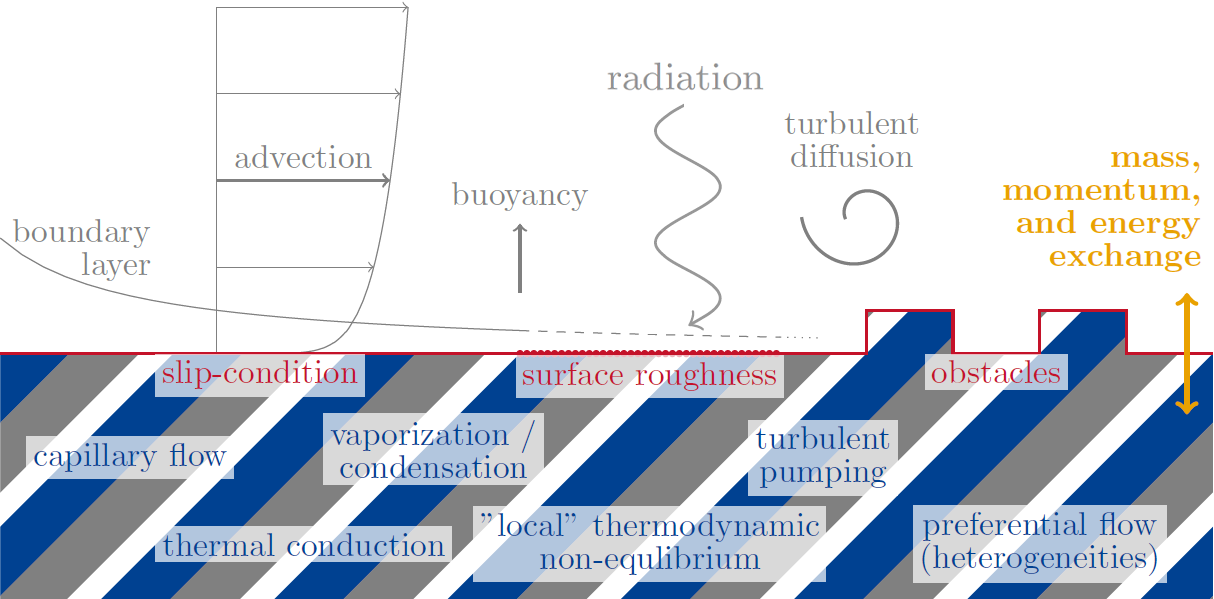
\includegraphics[width=\textwidth]{intropicture2.png}
	\caption[Exchange processes between free and porous-medium 
	flows]{Example of physical phenomena affecting the exchange processes 
		between a free-flow and a porous-medium flow. Figure source: 
		\cite{tesi:fetzer}.}
	\label{fig:intro}
\end{figure}

These studies can be exploited, for example, to better understand the process 
of soil salinization, that is one of the most serious agricultural problems in 
many arid and coastal areas in the world. It consists in the excessive 
accumulation of salt in the soil pores, with the consequence of a partial or 
complete loss of fertility. A limited amount of salt precipitation in the soil, 
due to evaporation of irrigation water, is inevitable, but a wrong water 
management could lead to salinity problems on the long term, especially in arid 
areas where irrigation is necessary to increase the production for food supply 
(see \cite{web:fao}). According to \cite{soil:munns}, more than 6\% of world's 
total land area is affected by salinization.
The part of the soil which is most involved in this problem is the one near the 
surface, hence it is important to study the interactions between the free-flow 
and the porous-medium flow that occur there. For example, 
\textcite{intro:salinization} have investigated the application of kinetic 
approaches to describe the salt precipitation in a coupled system.
\begin{figure}
	\centering
	\subfloat[]{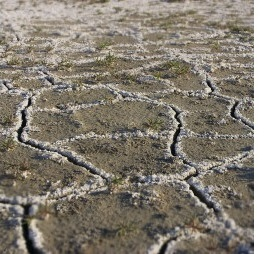
\includegraphics[height=0.22\textheight]{salinity.jpg} 
	\label{fig:soil}}
	\subfloat[]{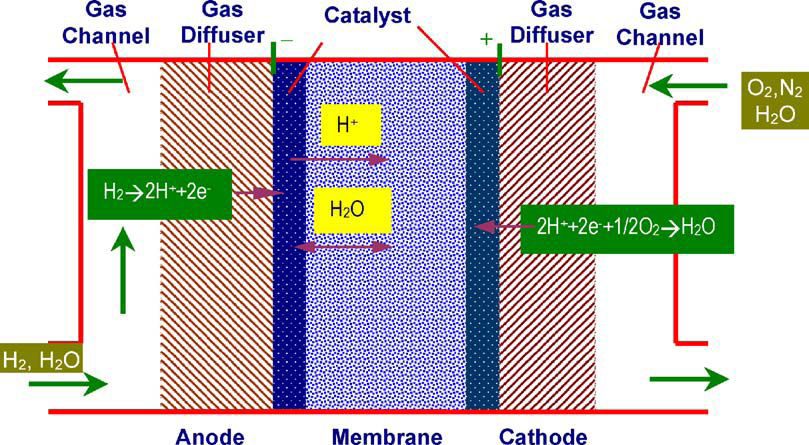
\includegraphics[height=0.22\textheight]{pem.png}\label{fig:pem}}
	\caption[Salt-affected soil and operation principle of PEM fuel 
	cells]{\protect\subref{fig:soil}: Salt-affected soil. Figure source: 
	\cite{web:fao}. \protect\subref{fig:pem}: Operation principle of PEM fuel 
	cells. Figure source: \cite{intro:pemfig}.}
	\label{fig:intro2}
\end{figure}

Switching to a technical framework, PEM (Proton Exchange Membrane) fuel cells 
represent a possible alternative power source that, in particular, could be 
used for transportation. In their design, transport and diffusion phenomena 
through gas channels and gas diffusers play an important role in the 
electrochemical reactions that determine the cell performances and efficiency. 
As we can see in Figure~\ref{fig:intro2}, reactant gases are transported 
through gas channels and supplied at the anode and cathode, then they diffuse 
into porous layers called gas diffusers, that should deliver them uniformly and 
efficiently to the catalyst layers, where reactions take place (see 
\cite{wu:fuelcell}, \cite{tesi:baber} and \cite{tesi:pem}). Protons are 
produced at the anode and transported through the membrane to react with oxygen 
at the cathode and produce water. The water management within the cells is of 
great importance because it is essential to have a certain level of humidity in 
the membrane in order to facilitate the transport of protons, but an excess of 
water could flood the catalyst layers, with the result of an inhibition of the 
reactions.
Because of the complex and compact geometry of PEM fuel cells, it is generally 
difficult and expensive to take measurements, thus mathematical and numerical 
models are helpful in order to better understand the mechanical, thermal and 
chemical phenomena that take place and this way improve the cell performances 
and lifetime.

Other examples of applications can be found in the fields of refrigeration of 
stored food \cite{intro:food}, cooling systems for aerospace engineering 
\cite{intro:aero}, ventilation of motorcycle helmets \cite{intro:discacim}, 
wind flow around buildings in urban environments \cite{intro:buildings} and 
hemodynamics \cite{intro:med}.

\section{State of the art}
In order to study these processes, in the following we focus on a system that 
involves two subdomains: the upper one with a free-flow and the lower one 
occupied by a porous-medium, as the one represented in Figure~\ref{fig:intro}.
At the interface between the two subdomains there is exchange of mass, momentum 
and energy.

Numerical studies of this coupled system can be performed with a 
\emph{single-domain} approach or with a \emph{two-domain} approach 
\cite{tesi:fetzer}.
Within the single-domain approach, the same equations are solved in the whole 
computational domain, including both the free-flow region and the 
porous-medium. A first possibility is to use the Navier-Stokes equations to model the 
fluid motion and thus to perform a direct numerical simulation (DNS) of the 
whole system. The porous-medium has to be resolved at the pore-scale, thus a 
detailed knowledge of the pore structure, which is not easy to obtain for real 
materials, is necessary. The computational effort is very high because 
of the strict spatial and temporal requirements of a DNS and it increases even 
more if the fluid is non-isothermal, multi-phase and multi-component. \textcite{intro:dns} and \textcite{intro:dns2} have performed DNS in 
porous-media domains using the lattice Boltzmann method, while \textcite{intro:yang} have performed coupled simulations considering idealised coarse porous materials.
A cheaper possibility for the case of laminar single-phase flows is to employ the Brinkman's equation 
\cite{intro:brinkman}, which is a superposition of the Stokes equations and 
Darcy's law, with a modified viscosity. %:
%\begin{equation}
%	-\nabla \cdot (\tilde{\mu} \nabla \mathbf{v}) + \mu 
%	\mathbf{K}^{-1}\mathbf{v} + \nabla p = \mathbf{f}.
%\end{equation}
Then the transition between the two 
regions can be expressed with a spatial variation of the involved physical 
parameters, either considering a transition region or admitting a discontinuous 
variation at the interface. \textcite{intro:shavit} proposed a modification of 
the Brinkman's equation and applied it to the case of shallow water flows over 
porous surfaces.

Within the two-domain approach, adopted also in this thesis, different sets of 
equations are used in the two subdomains and they are coupled imposing suitable 
conditions at the interface. This allows to keep separated models to describe phenomena that act on different temporal and spatial scales. The free-flow can be modelled with the Stokes 
equations, Navier-Stokes equations or RANS equations, depending on the flow 
regime. The porous-medium flow, instead, is usually described with a REV-scale approach, exploiting the 
Darcy's law or the Forchheimer's law when the Reynolds number is higher or the 
Richards equation. The interface could also be \emph{complex}, i.e. it could be 
allowed to store mass, for example to take into account drop formation (see 
\cite{tesi:baber}).

\textcite{intro:discacim} compared the performances of a single-domain approach with a penalization technique and a 
two-domain approach, using the Navier-Stokes equations and the Forchheimer's 
law to model an incompressible, single-phase, single-component flow. They 
concluded that the former is easier to implement, but the latter describes 
better the physics of the problem. Alternative approaches may exploit 
pore-networks models in the porous-medium subdomain, that allow to focus on the 
pore scale effects, avoiding the complexity of a DNS (see \cite{paper:kilian}).

\textcite{paper:mosthaf} proposed a Stokes/Darcy coupling concept for multi-phase, 
multi-component, non-isothermal flows. It is based on phenomenological arguments and it tries to be as close as possible to the 
imposition of thermodynamic equilibrium. \textcite{intro:davarzani}, instead, focused on the coupling in case of non-equilibrium conditions among phases.
\textcite{paper:fetzer} generalized the equilibrium concept to the case of 
turbulent flows, in \cite{tesi:fetzer} several turbulence models are tested and 
possible simplifications in the implementation of interface conditions are 
considered. The effects of turbulence, as well as the non-linear inertial 
effects of the Navier-Stokes equations, are sometimes neglected, for 
simplicity, 
but to model natural systems they must be included as they play an important 
role in most of the situations. Another aspect investigated in 
\cite{tesi:fetzer} is the influence of a rough interface between the two 
subdomains. In particular, both the effects of a sand-grain roughness and of 
periodical porous obstacles are studied.
Rough interfaces have been taken into account also in \cite{intro:kuzbek} and \cite{intro:kuz} to analyse heat transfer within a duct, while rough boundaries for free-flows are considered in \cite{lien:obstacles} to study flow paths around buildings, in \cite{intro:limnology}, in a limnological framework, and in \cite{intro:targui} to study heat exchangers.

Theoretical results concerning the well-posedness can be found in \cite{intro:disca}, for the Stokes/Darcy problem, and in \cite{intro:disca2009}, for the Navier-Stokes/Darcy problem. They are based on classical results for saddle-point problems. Regarding the numerical aspects, many different methods have been employed in literature. In \cite{intro:disca2009} several finite elements choices are considered, in \cite{tesi:mosthaf} the box method is used, while in \cite{tesi:fetzer} the same box method is compared to a combined staggered and collocated finite volumes method. In \cite{intro:disca} an iterative algorithm is proposed in order to decouple the two subdomains, while in \cite{intro:rybak} a temporal decoupling strategy is used.

\section{Content of the thesis}
In this thesis the focus is on the improvement, from the numerical point of view, of the free-flow model with respect to \cite{tesi:fetzer}. When the flow is in a turbulent regime, turbulent eddies develop near the interface and 
they cascade through consecutively smaller scales until the kinetic energy 
dissipates into internal thermal energy. Because of their location, they have 
a strong influence on the exchange processes between the two subdomains, so an 
accurate evaluation of their behaviour is of crucial importance. Improvements 
can be obtained with a refinement of the grid, but also by employing 
high order methods. In 
particular, in the discretization of the Navier-Stokes equations using finite 
volumes, the approximation used for the non linear term 
$\nabla \cdot (\mathbf{v} \mathbf{v}^\mathrm{T})$ plays a key role. A common and easy 
choice is to employ a first order upwind approximation for the 
\emph{transported} velocity, but this option can produce solutions with 
excessive numerical diffusion. Other possibilities are given by high order 
methods 
like the Linear Upwind Differencing (LUD) scheme, the Central Differencing (CD) 
scheme or the Quadratic Upstream Interpolation for Convective Kinetics (QUICK) 
scheme. Under specific conditions, they can produce 
accurate solutions but they have also shown to be unstable in certain 
situations and to produce overshoots or undershoots that 
may lead to unphysical values of quantities that for example have to be 
positive (see \cite{main:vermal}). With this in mind, our interest is in 
the Total Variation Diminishing (TVD) methods, a family of methods that has 
been derived with the purpose of providing a solution with a second order 
accuracy, but without any risk of numerical oscillations. They are called also 
high resolution methods.

In Chapter~\ref{chap:equations} the equations employed in the models will be 
presented, with particular attention to the free-flow equations. In 
Chapter~\ref{chap:discretization} the finite volume method will be described 
and, in Subsection~\ref{subsec:tvd}, the TVD methods will be introduced. At last, 
in Chapter~\ref{chap:results}, the numerical results will be shown. In 
particular, we will see the application of the TVD methods to the Navier-Stokes 
equations in comparison to the first order upwind scheme. Then two tests 
involving turbulent flows are presented and, finally, a more complex scenario involving 
obstacles at the interface between a free-flow region and a porous-medium is investigated.

The high order methods mentioned above have been implemented in the framework 
of the open-source simulator \DUMUX: DUNE for multi-$\{$phase, component, 
scale, physics, \dots$\}$ flow in porous-media, see \cite{dumux:tutti} and 
\cite{dumux:flemisch}. \DUMUX is an 
additional module of DUNE (Distributed and Unified Numerics Environment, 
\cite{web:dune}) and, through the use of an object-oriented design in 
conjunction with template programming, it provides a C++ environment that 
allows an efficient implementation of numerical models related to porous-media 
flows.

All the source code used for the simulations performed can be 
found at \url{https://git.iws.uni-stuttgart.de/dumux-pub/vescovini2019a}, 
together with the instructions to install the required software.
\chapter{Governing equations} \label{chap:equations} %mathematical model?
In this chapter the equations that have been used to model the 
free-flow and the porous-medium flow are presented. For the free-flow we start 
considering the incompressible Navier-Stokes equations to simulate laminar 
flows, then we move to the RANS equations employing the $k\text{-}\omega$ 
model as a turbulence model to deal with turbulent flows. For the porous-medium 
flow our choice is the Forchheimer's law, that is an extension of the more 
common Darcy's law to higher Reynolds numbers.
\section{Free-flow}
\subsection{Navier-Stokes equations}
The Navier-Stokes equations describe the motion of a Newtonian viscous fluid,
defining a relation between the following physical quantities:
\begin{itemize}
	\item $\varrho$, the density of the fluid  [$\si{kg/m^3}$],
	\item $\mathbf{v} = [u, v, w]^\mathrm{T}$, the velocity vector [$\si{m/s}$],
	\item $e$, the specific total energy [$\si{J/kg}$].
\end{itemize}
They can be derived starting from the general principles of conservation of 
mass:
\begin{equation} \label{eq:masscons}
\frac{d}{dt} \int_V \varrho \; dV = 0,
\end{equation}
the second Newton's law:
\begin{equation} \label{eq:2newton}
\frac{d}{dt} \int_V \varrho \mathbf{v} \; dV = \int_V \varrho \mathbf{b} \; dV 
+ 
\int_{\partial V} \sigma \mathbf{n} \; dA
\end{equation}
and the first law of thermodynamics:
\begin{equation} \label{eq:firstthermo}
\frac{d}{dt} \int_V e \; dV = \dot{Q} + \dot{W}
\end{equation}
for an infinitesimal volume $V$. In the equation \eqref{eq:2newton} the vector 
$\mathbf{b}$ represents possible external volume forces per unit of mass, for 
example the gravity $\mathbf{g}$. $\sigma$ is the Cauchy stress tensor 
and 
$\mathbf{n}$ is the outward unit vector normal to the surface $\partial V$ of 
$V$, while in the equation \eqref{eq:firstthermo} $\dot{Q}$ is the net rate of 
heat added to the fluid and $\dot{W}$ is the net rate of work done on the fluid.

For viscous fluids we can identify two contributions in the Cauchy stress 
tensor:
\begin{equation}
\sigma = -p\mathbb{1} + \tau,
\end{equation}
$-p\mathbb{1}$ is a contribution due to pressure, while $\tau$ is 
the viscous stress tensor, for which the constitutive relation of Newtonian 
fluids is used:
\begin{equation}
\tau = 2\mu \mathbf{S} + 
\lambda (\nabla \cdot \mathbf{v}) \mathbb{1},
\end{equation}
where $\mu$ is the dynamic viscosity [$\si{\pascal\second}$], $\lambda$ 
is a dilatation factor and $\mathbf{S}$ is the symmetric strain rate tensor:
\begin{equation*}
\mathbf{S} = \frac{\nabla \mathbf{v} + \nabla \mathbf{v}^\mathrm{T}}{2}.
\end{equation*} 
Moreover we define the kinematic viscosity 
[$\si{m^2/s}$] as
\begin{equation}
\nu = \frac{\mu}{\varrho}.
\end{equation}

We want to deal with incompressible fluids, so that the density is taken 
constant and not related to the pressure through a state equation. Thus the 
energy equation is not needed anymore and we can exclude it from the system. 
Notice that with this assumption $p$ is no more the thermodynamic pressure.
Using these assumptions from the balance equations 
\eqref{eq:masscons} and \eqref{eq:2newton} we obtain the Navier-Stokes 
equations:
\begin{align}
\label{eq:nsmass} \nabla \cdot \mathbf{v} = 0&\\
\label{eq:nsmom} \frac{\partial \mathbf{v}}{\partial t} + \nabla 
\cdot (\mathbf{v} \mathbf{v}^\mathrm{T}) - \nabla \cdot (\nu \nabla 
\mathbf{v}) + \frac{1}{\varrho}\nabla p  -\mathbf{g} = \mathbf{0}&
\end{align}
All the computations needed to obtain these equations can be found in any book 
of fluid mechanics, for example in \cite{main:vermal}. The continuity equations 
reduces to an incompressibility constraint \eqref{eq:nsmass} that is enforced 
in the momentum equation through the pressure that acts as a Lagrangian 
multiplier. The second term of the momentum equation \eqref{eq:nsmom} is 
non-linear and represents the advection that the velocity enforces on itself, 
while the third one is a diffusive term that express the action of the 
viscosity.
%
\subsubsection{Boundary conditions}
When the equations \eqref{eq:nsmass} and \eqref{eq:nsmom} are solved in a 
bounded domain $\Omega_\text{ff}$, suitable conditions have to be provided at 
the boundary $\partial \Omega_\text{ff}$, depending on the situation that we 
want to model. Common choices, adopted also in Chapter~\ref{chap:results}, are:
\begin{itemize}
	\item on inflow boundaries, Dirichlet conditions are imposed to the 
	velocity:
	\begin{equation} \label{eq:inflow}
		\mathbf{v} = \mathbf{v}_\text{in},
	\end{equation}
	\item on solid walls, homogeneous Dirichlet conditions are imposed to the 
	velocity (also called no-slip conditions):
	\begin{equation} \label{eq:noslip}
		\mathbf{v} = \mathbf{0},
	\end{equation}
	\item on outflow boundaries, natural boundary conditions are imposed, 
	resulting in the following prescription for the stress :
	\begin{equation}
		\sigma \mathbf{n} = -p\mathbf{n}+2\mu \mathbf{Sn} = \varrho\mathbf{d},
	\end{equation}
	where $\mathbf{n}$ is the outward unit vector normal to the surface. 
	However outflow boundary conditions are usually located where the flow is 
	almost unidirectional and the surface stresses are known, so, especially 
	when using the finite volumes method, they are replaced by:
	\begin{equation} \label{eq:outflow}
	(\nabla \mathbf{v})\mathbf{n} = \mathbf{0}, \quad p = p_\text{ext},
	\end{equation}
	thus fixing a a zero-gradient condition for the velocity and imposing a 
	Dirichlet condition to the pressure (see \cite{main:vermal}).
\end{itemize}
Moreover it is usually useful to take advantage of symmetries in the flow 
field, 
when they are known because of the domain and of the other boundary conditions. 
For example, in order to model a flow in a pipe, we can impose the following 
symmetry conditions along the centre of the domain and consider only half of it:
\begin{equation}
\nabla p \cdot \mathbf{n} = 0, \quad \nabla v_t \cdot \mathbf{n} = 0, \quad
v_n = 0,
\end{equation}
where $v_t$ an $v_n$ are the tangential and normal components of the velocity.
%
\subsubsection{Reynolds number}
If we consider the non-dimensional form of equation \eqref{eq:nsmom}, scaling 
the lengths by a reference quantity $L$ and the velocities by a reference 
quantity $U$, and if we neglect the gravity, we obtain
\begin{equation} \label{eq:momnondim}
	\frac{\partial{\tilde{\mathbf{v}}}}{\partial \tilde{t}} + \tilde{\nabla} 
	\cdot (\tilde{\mathbf{v}} \tilde{\mathbf{v}}^\mathrm{T}) - \tilde{\nabla} 
	\cdot \bigg(\frac{1}{Re} \tilde{\nabla} \tilde{\mathbf{v}}\bigg) + 
	\tilde{\nabla} 
	\tilde{p} = 0
\end{equation}
where the non-dimensional number $Re$ that multiplies the viscous term is the 
Reynolds number and it is defined as:
\begin{equation}
Re = \frac{UL}{\nu}.
\end{equation}
This quantity plays an important role in the behaviour of the solution of the 
Navier-Stokes equations since it expresses the ratio between the inertia forces 
and the viscous forces. This can be easily seen in the equation 
\eqref{eq:momnondim} since, when $Re\gg 1$, the viscous term loses 
importance with respect to the advective one and vice versa.

If $Re < 1$ we have a creeping flow and generally the advection term can 
be neglected, reducing the Navier-Stokes equations to the Stokes equations, 
that are much simpler to analyse and to solve because they are linear. The 
assumption of creeping flow is common in porous-media models, as we will 
see in Section~\ref{sec:pm}. If $Re>1$ we have a laminar flow, which is 
characterized by a well-ordered viscosity-dominated motion, with adjacent 
layers of the fluid that slide with little interaction between each others.
There exists a critical value $Re_c$ such that when $Re>Re_c$ a 
transition from a laminar to a turbulent flow regime starts to take place, but 
this threshold value is very problem dependent as it is affected by the 
geometry of the domain and by the boundary conditions imposed.
%
\subsection{Turbulence and RANS equations}
Turbulence is characterized by an irregular, chaotic and intermittent 
behaviour, that shows space and time fluctuations of the physical quantities 
related to the flow, as we can see in Figure~\ref{fig:fluctuations}. Due to 
this complexity, turbulence is usually studied with 
a statistical approach, relying on the theory developed by Kolmogorov 
in 1941 \cite{turbo:kolmogorov}. A wider description of turbulence can be 
found for example in \cite{main:pope}, \cite{main:wilcox} or 
\cite{main:davidson}.
\begin{figure}[ht]
	\centering
	% This file was created by matlab2tikz.
%
\begin{tikzpicture}

\begin{axis}[%
width=0.951\widthsette,
height=0.75\widthsette,
at={(0\widthsette,0\widthsette)},
scale only axis,
xmin=0.0003,
xmax=4.0023,
xlabel={time [s]},
ymin=10,
ymax=22,
ylabel={velocity [m/s]},
axis background/.style={fill=white},
xmajorgrids,
ymajorgrids
]
\addplot [color=black, forget plot]
  table[row sep=crcr]{%
0.0003	15.86\\
0.0063	14.5779\\
0.0123	13.6604\\
0.0183	12.8875\\
0.0243	12.4176\\
0.0303	12.6551\\
0.0363	14.0939\\
0.0423	16.3555\\
0.0483	16.7261\\
0.0543	15.9008\\
0.0603	14.9808\\
0.0663	13.9689\\
0.0723	13.455\\
0.0783	13.8104\\
0.0843	14.4593\\
0.0903	14.7927\\
0.0963	14.7728\\
0.1023	14.7752\\
0.1083	14.8455\\
0.1143	14.7653\\
0.1203	14.5008\\
0.1263	13.9457\\
0.1323	13.3764\\
0.1383	13.1549\\
0.1443	13.2625\\
0.1503	13.4964\\
0.1563	13.7114\\
0.1623	13.7333\\
0.1683	13.4597\\
0.1743	12.8486\\
0.1803	12.0619\\
0.1863	11.4672\\
0.1923	11.2568\\
0.1983	11.151\\
0.2043	10.9918\\
0.2103	10.8552\\
0.2163	10.8836\\
0.2223	11.1893\\
0.2283	11.6717\\
0.2343	12.5418\\
0.2403	14.2533\\
0.2463	16.6234\\
0.2523	17.7437\\
0.2583	17.3127\\
0.2643	16.9952\\
0.2703	16.7505\\
0.2763	15.918\\
0.2823	14.8688\\
0.2883	14.2\\
0.2943	14.2536\\
0.3003	14.7781\\
0.3063	14.6915\\
0.3123	13.9757\\
0.3183	14.1038\\
0.3243	15.1628\\
0.3303	15.7353\\
0.3363	15.4467\\
0.3423	15.1117\\
0.3483	15.3946\\
0.3543	16.3112\\
0.3603	17.4856\\
0.3663	17.446\\
0.3723	16.4975\\
0.3783	16.1235\\
0.3843	15.6614\\
0.3903	14.7967\\
0.3963	14.4551\\
0.4023	14.7712\\
0.4083	15.3108\\
0.4143	15.536\\
0.4203	15.4543\\
0.4263	15.2118\\
0.4323	15.1857\\
0.4383	15.3773\\
0.4443	15.9158\\
0.4503	17.8316\\
0.4563	19.399\\
0.4623	18.32\\
0.4683	17.3181\\
0.4743	17.402\\
0.4803	17.0503\\
0.4863	16.7268\\
0.4923	17.2966\\
0.4983	17.7082\\
0.5043	17.2802\\
0.5103	16.3873\\
0.5163	15.5827\\
0.5223	16.1701\\
0.5283	17.6804\\
0.5343	17.8357\\
0.5403	16.7855\\
0.5463	16.6724\\
0.5523	16.6855\\
0.5583	16.0132\\
0.5643	15.2843\\
0.5703	15.2546\\
0.5763	15.5366\\
0.5823	15.5601\\
0.5883	15.4162\\
0.5943	15.5954\\
0.6003	16.4528\\
0.6063	17.7084\\
0.6123	18.4371\\
0.6183	18.3985\\
0.6243	17.8188\\
0.6303	17.2643\\
0.6363	17.6704\\
0.6423	18.14\\
0.6483	17.7004\\
0.6543	16.7625\\
0.6603	15.7686\\
0.6663	15.0375\\
0.6723	14.9552\\
0.6783	15.9977\\
0.6843	16.8789\\
0.6903	16.1598\\
0.6963	15.5031\\
0.7023	16.0681\\
0.7083	16.7218\\
0.7143	16.3755\\
0.7203	15.6385\\
0.7263	15.2752\\
0.7323	15.2756\\
0.7383	15.0903\\
0.7443	14.6455\\
0.7503	14.1703\\
0.7563	14.021\\
0.7623	14.1074\\
0.7683	14.4324\\
0.7743	14.9701\\
0.7803	15.4744\\
0.7863	15.6458\\
0.7923	15.6543\\
0.7983	15.6902\\
0.8043	15.603\\
0.8103	15.6832\\
0.8163	15.9489\\
0.8223	16.5783\\
0.8283	17.6392\\
0.8343	18.2035\\
0.8403	18.4581\\
0.8463	18.0874\\
0.8523	17.6087\\
0.8583	17.6756\\
0.8643	17.6851\\
0.8703	18.0928\\
0.8763	18.9178\\
0.8823	19.29\\
0.8883	18.7701\\
0.8943	18.178\\
0.9003	17.7217\\
0.9063	17.0352\\
0.9123	16.2568\\
0.9183	15.6914\\
0.9243	15.4099\\
0.9303	15.4549\\
0.9363	15.483\\
0.9423	15.0668\\
0.9483	14.3225\\
0.9543	14.0247\\
0.9603	14.9969\\
0.9663	16.6177\\
0.9723	17.5198\\
0.9783	17.9927\\
0.9843	19.2434\\
0.9903	20.1417\\
0.9963	19.8787\\
1.0023	19.7383\\
1.0083	19.778\\
1.0143	19.5067\\
1.0203	18.8249\\
1.0263	18.6157\\
1.0323	19.306\\
1.0383	19.388\\
1.0443	19.0189\\
1.0503	18.5446\\
1.0563	17.9869\\
1.0623	17.8616\\
1.0683	18.0275\\
1.0743	17.914\\
1.0803	17.4873\\
1.0863	17.3115\\
1.0923	17.2159\\
1.0983	16.7717\\
1.1043	16.7897\\
1.1103	17.1446\\
1.1163	16.9313\\
1.1223	16.5983\\
1.1283	16.6969\\
1.1343	17.2994\\
1.1403	18.171\\
1.1463	18.2113\\
1.1523	17.296\\
1.1583	16.3942\\
1.1643	16.3234\\
1.1703	16.5367\\
1.1763	16.4588\\
1.1823	16.6058\\
1.1883	17.4649\\
1.1943	18.3317\\
1.2003	18.549\\
1.2063	18.565\\
1.2123	18.472\\
1.2183	18.1037\\
1.2243	17.987\\
1.2303	18.1333\\
1.2363	17.9932\\
1.2423	17.6615\\
1.2483	17.4939\\
1.2543	17.3346\\
1.2603	17.0236\\
1.2663	16.5317\\
1.2723	15.9516\\
1.2783	15.609\\
1.2843	15.5576\\
1.2903	15.6172\\
1.2963	15.5174\\
1.3023	14.9878\\
1.3083	14.0482\\
1.3143	12.9265\\
1.3203	11.9061\\
1.3263	11.3348\\
1.3323	11.7104\\
1.3383	13.6311\\
1.3443	15.4829\\
1.3503	15.8352\\
1.3563	16.0726\\
1.3623	16.0857\\
1.3683	16.2257\\
1.3743	18.4147\\
1.3803	18.7568\\
1.3863	17.4431\\
1.3923	16.5547\\
1.3983	14.9914\\
1.4043	13.7956\\
1.4103	13.883\\
1.4163	15.1158\\
1.4223	16.2528\\
1.4283	16.7131\\
1.4343	17.0106\\
1.4403	17.4296\\
1.4463	17.3157\\
1.4523	16.618\\
1.4583	16.0574\\
1.4643	15.5473\\
1.4703	14.9971\\
1.4763	14.9418\\
1.4823	15.9284\\
1.4883	17.7894\\
1.4943	19.1699\\
1.5003	19.1514\\
1.5063	18.4303\\
1.5123	19.0803\\
1.5183	19.0747\\
1.5243	18.1214\\
1.5303	18.4665\\
1.5363	18.6808\\
1.5423	18.6865\\
1.5483	18.3973\\
1.5543	18.0313\\
1.5603	18.4609\\
1.5663	18.584\\
1.5723	18.1613\\
1.5783	17.4144\\
1.5843	16.3114\\
1.5903	15.3974\\
1.5963	15.7673\\
1.6023	17.4384\\
1.6083	18.8497\\
1.6143	18.5874\\
1.6203	17.8947\\
1.6263	17.9242\\
1.6323	17.6697\\
1.6383	17.4096\\
1.6443	17.0035\\
1.6503	16.162\\
1.6563	15.1234\\
1.6623	13.7363\\
1.6683	12.2476\\
1.6743	11.4034\\
1.6803	11.31\\
1.6863	11.746\\
1.6923	12.575\\
1.6983	12.8235\\
1.7043	12.1165\\
1.7103	11.2387\\
1.7163	10.6103\\
1.7223	10.3114\\
1.7283	10.7632\\
1.7343	13.1243\\
1.7403	16.2055\\
1.7463	17.044\\
1.7523	16.6977\\
1.7583	17.2349\\
1.7643	17.6414\\
1.7703	17.5848\\
1.7763	17.5219\\
1.7823	17.2514\\
1.7883	17.2231\\
1.7943	17.3389\\
1.8003	17.0654\\
1.8063	16.3686\\
1.8123	15.7027\\
1.8183	15.3444\\
1.8243	15.3445\\
1.8303	15.4408\\
1.8363	15.1064\\
1.8423	14.7907\\
1.8483	14.872\\
1.8543	14.8277\\
1.8603	14.3461\\
1.8663	13.7831\\
1.8723	13.1416\\
1.8783	12.3305\\
1.8843	11.8102\\
1.8903	12.0356\\
1.8963	12.7216\\
1.9023	12.4762\\
1.9083	11.5936\\
1.9143	13.6117\\
1.9203	18.173\\
1.9263	18.8767\\
1.9323	17.1844\\
1.9383	17.281\\
1.9443	18.2846\\
1.9503	17.8632\\
1.9563	17.0892\\
1.9623	16.6851\\
1.9683	16.9871\\
1.9743	17.357\\
1.9803	16.6897\\
1.9863	16.0727\\
1.9923	16.3268\\
1.9983	16.9649\\
2.0043	17.8683\\
2.0103	18.1467\\
2.0163	17.736\\
2.0223	17.5434\\
2.0283	17.8539\\
2.0343	18.7492\\
2.0403	19.3437\\
2.0463	18.5694\\
2.0523	17.8653\\
2.0583	17.6271\\
2.0643	17.2334\\
2.0703	16.5327\\
2.0763	15.6194\\
2.0823	15.0293\\
2.0883	14.5965\\
2.0943	13.8245\\
2.1003	12.9351\\
2.1063	12.4345\\
2.1123	12.4489\\
2.1183	12.4987\\
2.1243	12.1763\\
2.1303	11.949\\
2.1363	12.24\\
2.1423	13.1771\\
2.1483	14.4033\\
2.1543	15.3406\\
2.1603	15.6406\\
2.1663	15.9244\\
2.1723	16.9545\\
2.1783	17.1347\\
2.1843	16.5889\\
2.1903	16.3542\\
2.1963	15.8723\\
2.2023	15.1942\\
2.2083	14.6928\\
2.2143	14.298\\
2.2203	13.8325\\
2.2263	13.2055\\
2.2323	12.5197\\
2.2383	11.9895\\
2.2443	11.8806\\
2.2503	12.8976\\
2.2563	15.8567\\
2.2623	18.2655\\
2.2683	17.719\\
2.2743	16.7296\\
2.2803	16.0351\\
2.2863	15.493\\
2.2923	15.3613\\
2.2983	15.4564\\
2.3043	15.2948\\
2.3103	14.9102\\
2.3163	14.4463\\
2.3223	13.9853\\
2.3283	13.8349\\
2.3343	13.9854\\
2.3403	14.2419\\
2.3463	14.5512\\
2.3523	14.7789\\
2.3583	14.4919\\
2.3643	13.6437\\
2.3703	13.5709\\
2.3763	15.6555\\
2.3823	18.2158\\
2.3883	18.6401\\
2.3943	18.9101\\
2.4003	18.7038\\
2.4063	18.2354\\
2.4123	17.8216\\
2.4183	17.619\\
2.4243	17.6751\\
2.4303	17.4953\\
2.4363	16.268\\
2.4423	15.799\\
2.4483	18.3422\\
2.4543	19.5704\\
2.4603	18.0564\\
2.4663	16.438\\
2.4723	15.5798\\
2.4783	15.7604\\
2.4843	15.6362\\
2.4903	14.9156\\
2.4963	14.0839\\
2.5023	13.2795\\
2.5083	12.7439\\
2.5143	12.9944\\
2.5203	14.8865\\
2.5263	17.7526\\
2.5323	18.2359\\
2.5383	18.3272\\
2.5443	18.6022\\
2.5503	17.6411\\
2.5563	16.9723\\
2.5623	16.6336\\
2.5683	15.6604\\
2.5743	14.2481\\
2.5803	12.8915\\
2.5863	12.2525\\
2.5923	12.302\\
2.5983	12.4125\\
2.6043	12.6377\\
2.6103	13.1299\\
2.6163	13.8053\\
2.6223	14.538\\
2.6283	15.2473\\
2.6343	15.5391\\
2.6403	14.668\\
2.6463	13.4119\\
2.6523	13.0032\\
2.6583	14.0169\\
2.6643	16.0353\\
2.6703	17.6362\\
2.6763	16.7815\\
2.6823	16.4306\\
2.6883	16.5854\\
2.6943	16.4898\\
2.7003	17.1528\\
2.7063	18.1666\\
2.7123	18.3997\\
2.7183	18.9133\\
2.7243	19.8627\\
2.7303	19.555\\
2.7363	18.9644\\
2.7423	18.4798\\
2.7483	18.2803\\
2.7543	18.5642\\
2.7603	18.5385\\
2.7663	18.0276\\
2.7723	17.5834\\
2.7783	17.6391\\
2.7843	17.7646\\
2.7903	17.7169\\
2.7963	17.9831\\
2.8023	17.6376\\
2.8083	16.4791\\
2.8143	15.4324\\
2.8203	15.1645\\
2.8263	16.4503\\
2.8323	18.9688\\
2.8383	19.6478\\
2.8443	18.7021\\
2.8503	18.1203\\
2.8563	17.2212\\
2.8623	16.2436\\
2.8683	16.2262\\
2.8743	16.6615\\
2.8803	16.542\\
2.8863	16.2782\\
2.8923	16.251\\
2.8983	15.9217\\
2.9043	16.0308\\
2.9103	17.0109\\
2.9163	17.2385\\
2.9223	16.3355\\
2.9283	14.5068\\
2.9343	12.8464\\
2.9403	12.5848\\
2.9463	13.2168\\
2.9523	13.7715\\
2.9583	13.5817\\
2.9643	13.7284\\
2.9703	16.5018\\
2.9763	18.6876\\
2.9823	17.6662\\
2.9883	18.254\\
2.9943	19.0558\\
3.0003	17.5674\\
3.0063	16.3991\\
3.0123	16.5304\\
3.0183	17.0515\\
3.0243	16.9502\\
3.0303	16.5594\\
3.0363	16.6198\\
3.0423	16.2703\\
3.0483	15.7463\\
3.0543	15.602\\
3.0603	15.3706\\
3.0663	14.9132\\
3.0723	14.7599\\
3.0783	14.9564\\
3.0843	15.4864\\
3.0903	15.9697\\
3.0963	16.869\\
3.1023	17.1673\\
3.1083	16.0658\\
3.1143	15.8307\\
3.1203	15.8072\\
3.1263	15.6489\\
3.1323	15.8434\\
3.1383	15.461\\
3.1443	14.9123\\
3.1503	15.0308\\
3.1563	15.3756\\
3.1623	14.8817\\
3.1683	13.9436\\
3.1743	13.8028\\
3.1803	14.1165\\
3.1863	13.797\\
3.1923	13.3683\\
3.1983	13.4228\\
3.2043	13.6877\\
3.2103	13.4553\\
3.2163	12.3848\\
3.2223	11.3361\\
3.2283	11.0107\\
3.2343	11.9399\\
3.2403	14.3954\\
3.2463	15.9452\\
3.2523	14.4128\\
3.2583	13.1608\\
3.2643	13.0111\\
3.2703	13.1883\\
3.2763	13.7113\\
3.2823	15.0645\\
3.2883	16.519\\
3.2943	17.5202\\
3.3003	18.0494\\
3.3063	18.3518\\
3.3123	19.2229\\
3.3183	18.8023\\
3.3243	17.9055\\
3.3303	18.3903\\
3.3363	19.1389\\
3.3423	19.3848\\
3.3483	19.0849\\
3.3543	18.596\\
3.3603	17.9064\\
3.3663	16.6334\\
3.3723	15.7149\\
3.3783	15.2743\\
3.3843	15.2421\\
3.3903	15.8078\\
3.3963	16.3511\\
3.4023	16.1769\\
3.4083	15.5324\\
3.4143	14.9256\\
3.4203	14.8162\\
3.4263	14.9654\\
3.4323	14.809\\
3.4383	14.7284\\
3.4443	14.0218\\
3.4503	13.0674\\
3.4563	13.0774\\
3.4623	13.8606\\
3.4683	14.2415\\
3.4743	14.6959\\
3.4803	16.7953\\
3.4863	18.2302\\
3.4923	17.5177\\
3.4983	16.9454\\
3.5043	16.5351\\
3.5103	16.382\\
3.5163	16.3961\\
3.5223	16.0244\\
3.5283	15.5109\\
3.5343	15.0234\\
3.5403	14.686\\
3.5463	15.1045\\
3.5523	15.4758\\
3.5583	15.2949\\
3.5643	15.6651\\
3.5703	16.9748\\
3.5763	17.7086\\
3.5823	17.3164\\
3.5883	17.0658\\
3.5943	16.8035\\
3.6003	16.3418\\
3.6063	16.1533\\
3.6123	16.6961\\
3.6183	17.7745\\
3.6243	18.0856\\
3.6303	17.4901\\
3.6363	17.3521\\
3.6423	17.6591\\
3.6483	17.6563\\
3.6543	17.286\\
3.6603	17.3956\\
3.6663	18.6284\\
3.6723	19.3784\\
3.6783	18.7531\\
3.6843	18.1549\\
3.6903	18.1651\\
3.6963	18.2956\\
3.7023	18.0641\\
3.7083	17.5242\\
3.7143	17.4159\\
3.7203	18.347\\
3.7263	19.9416\\
3.7323	20.9975\\
3.7383	19.581\\
3.7443	17.4912\\
3.7503	16.6143\\
3.7563	16.6011\\
3.7623	16.4596\\
3.7683	16.5521\\
3.7743	16.766\\
3.7803	16.5696\\
3.7863	16.6001\\
3.7923	17.0069\\
3.7983	16.6306\\
3.8043	15.6609\\
3.8103	15.0956\\
3.8163	15.0208\\
3.8223	15.2091\\
3.8283	15.8381\\
3.8343	16.51\\
3.8403	16.5689\\
3.8463	16.1556\\
3.8523	15.6363\\
3.8583	15.6787\\
3.8643	16.9571\\
3.8703	18.6895\\
3.8763	19.055\\
3.8823	17.9611\\
3.8883	16.803\\
3.8943	15.8989\\
3.9003	14.9991\\
3.9063	13.7844\\
3.9123	13.5865\\
3.9183	15.3834\\
3.9243	16.3722\\
3.9303	15.9978\\
3.9363	15.9879\\
3.9423	16.532\\
3.9483	17.041\\
3.9543	18.5642\\
3.9603	19.4291\\
3.9663	18.8596\\
3.9723	18.8303\\
3.9783	18.9261\\
3.9843	18.8079\\
3.9903	18.2912\\
3.9963	17.7634\\
4.0023	17.4271\\
};
\end{axis}
\end{tikzpicture}%
	\caption[Fluctuating velocity in a turbulent flow]{Example of fluctuating 
	velocity in a turbulent flow.} %Re=1e7
	\label{fig:fluctuations}
\end{figure}

The first thing that can be observed in a turbulent flow is the presence of 
many three-dimensional eddies, that enhance the dispersive and mixing 
properties 
of the fluid. 
They cover a wide spectrum of length scales, in which we can identify 
three distinct bands; in the first one, corresponding to large scales, 
comparable to the size of the domain, there is an injection of kinetic energy 
and eddies are generated. Then there is an intermediate band in which the 
convection is dominant and eddies shrink without a significant loss of energy. 
The third band corresponds to the smallest scales at which eddies are present. 
Indeed, once they reach a certain size, the effect of the viscosity starts to 
be relevant and we assist to a dissipation of the kinetic energy of the eddies 
into internal thermal energy. So, globally, energy is transferred from large 
scales to small ones, until it gets dissipated; this process is known as 
the Richardson energy cascade (Figure~\ref{fig:cascade}).
\begin{figure}%[t]
	\centering
%	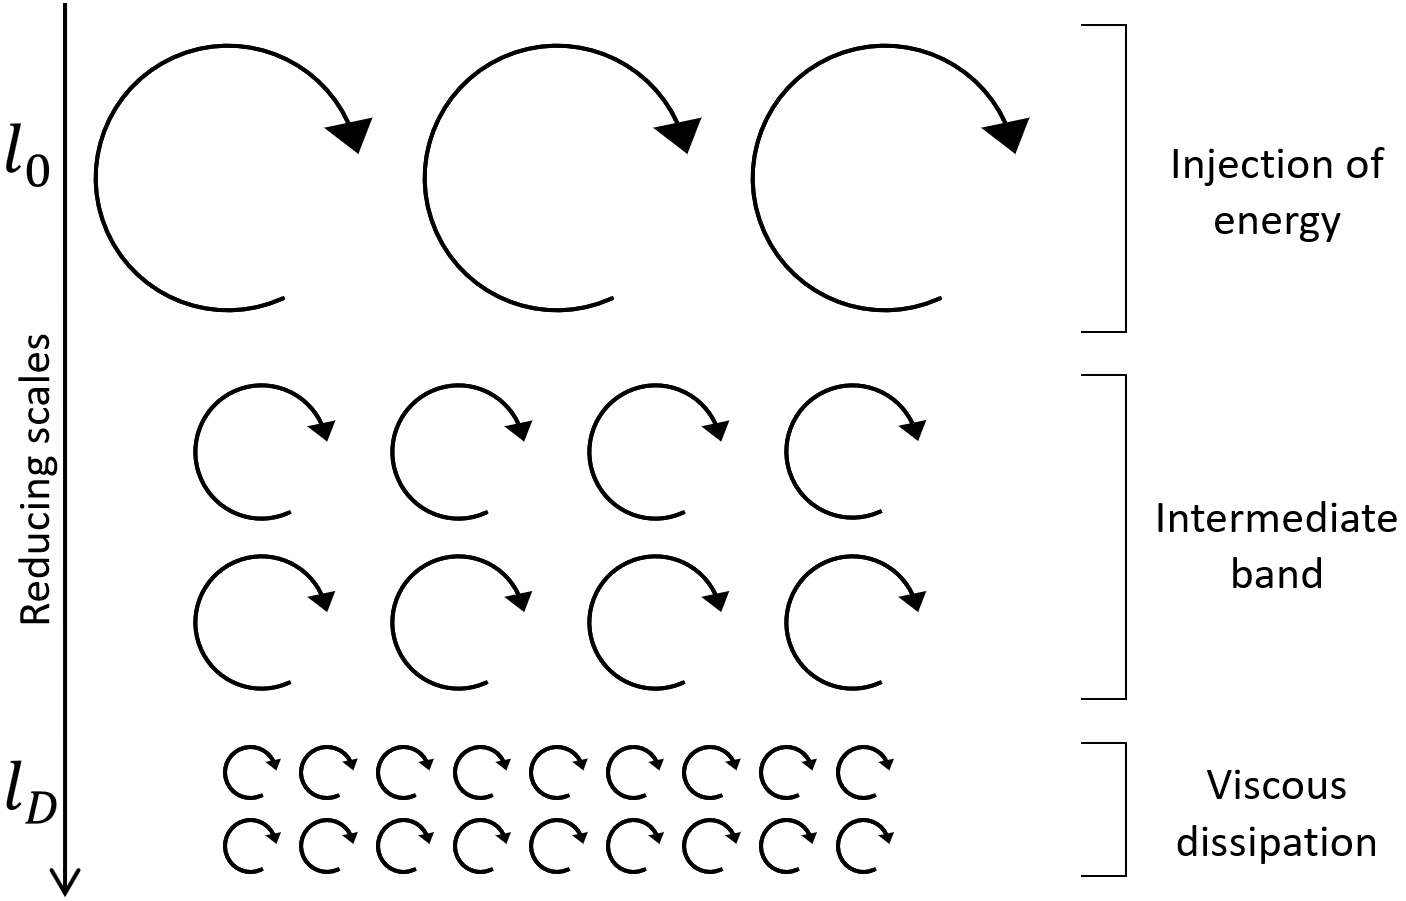
\includegraphics[width=\textwidth]{richardsoncascade.png}
	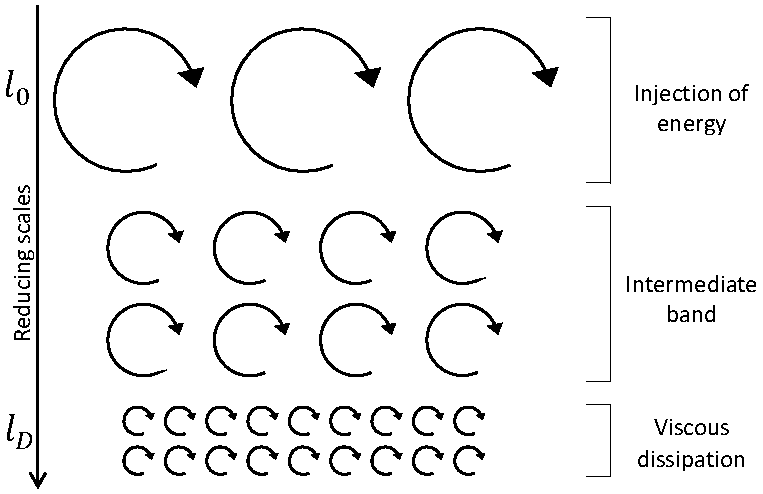
\includegraphics[width=\textwidth]{richardsoncascade.pdf}
	\caption[Richardson energy cascade]{Scheme of the Richardson energy 
	cascade.}
	\label{fig:cascade}
\end{figure}
%

\subsubsection{Simulation of turbulent flows}
From the Kolmogorov theory we can obtain useful information for the simulation 
of turbulent flows. Let us indicate with $l_0$ the length scale at which the 
eddies are generated and with $l_D$ the length scale at which they dissipate. 
Then according to \cite{turbo:kolmogorov} it can be obtained that
\begin{equation} \label{eq:scaleratio}
	\frac{l_0}{l_D} \sim Re^\frac{3}{4}.
\end{equation}
If we want to perform a reliable simulation of a turbulent flow using the 
Navier-Stokes equations \eqref{eq:nsmass}-\eqref{eq:nsmom} we need a grid with 
a spatial resolution sufficient to resolve all the eddies until the smallest 
ones, otherwise we would neglect the important information about the viscous 
dissipation of these structures. Assuming to have a domain of size comparable 
to $l_0$, then we need a size of the cells of the grid not bigger than $l_D$ and
from \eqref{eq:scaleratio} we deduce that we need at least $Re^\frac{3}{4}$ 
cells in each of the three dimensions of a domain. Because of the fluctuating 
behaviour of turbulence, we always have to perform unsteady simulations, so let 
us denote with $t_0$ the characteristic time of evolution of the eddies at 
$l_0$ and with $t_D$ the characteristic time of evolution of the eddies at 
$l_D$. Again from \cite{turbo:kolmogorov} we have that
\begin{equation}
\frac{t_0}{t_D} \sim Re^\frac{1}{2}.
\end{equation}
The total number of operations needed in a simulation $N$ can be considered 
proportional to:
\begin{equation}
	N \sim  N_t N_\text{elem},
\end{equation}
where $N_t$ is the total number of time-steps and $N_\text{elem}$ is the total 
number 
of elements in the grid and. From the previous relations we obtain:
\begin{equation}
	N \sim N_t N_\text{elem} \sim \frac{t_0}{t_D} \bigg(\frac{l_0}{l_D}\bigg)^3 
	= Re^\frac{11}{4}.
\end{equation}
%so we need at least $Re^\frac{1}{2}$ time-steps. Globally we end up with a 
%number of 
%degrees of freedom of the order of
%\begin{equation}
%	\# dof \sim \frac{t_0}{t_D} \bigg(\frac{l_0}{l_D}\bigg)^3 = Re^\frac{11}{4}.
%\end{equation}
Reynolds numbers can be easily of the order of $\num{e6}$ or greater in common 
situations, so even with this rough estimate we can see that the computational 
effort for these simulations, called Direct Numerical Simulations (DNS), is 
usually very high. Moreover such a detailed information that we would obtain 
usually goes beyond the real need in many applications, therefore other 
approaches have been developed in order to solve this issue, such as the one 
proposed by the RANS equations.
%
\subsubsection{RANS equations}
The Reynolds Averaged Navier-Stokes (RANS) equations focus on the mean flow 
field, avoiding to simulate all the eddies but without forgetting to take into 
account their effect. In engineering applications this is the most common way 
to simulate turbulent flows because it is cheap and usually the mean 
information is enough for many applications, but we must not forget that 
the obtained result is not the flow field as it appears in realty.
In case that more detail is needed, another approach is given by the Large 
Eddy Simulations (LES), that consist in applying a filter to the Navier-Stokes 
equation that let resolve the eddies until a certain threshold.

The first move towards the RANS equations is to decompose each instantaneous 
quantity in the sum of a mean value and a fluctuation: 
\begin{equation} \label{eq:decomp}
\mathbf{v} = \bar{\mathbf{v}} + \mathbf{v}', \quad p = \bar{p} + p'
\end{equation}
According to \cite{main:vermal} the mean value can be obtained with a time 
average over a long time interval 
for steady flows, while it is obtained with an ensemble average for unsteady 
flows, so that by definition
\begin{equation}
	\overline{\mathbf{v}'} = \mathbf{0}, \quad \overline{p'}=0.
\end{equation}
We want equations for the mean 
velocity $\bar{\mathbf{v}}$ and the mean pressure $\bar{p}$, so we apply the 
average operation to the Navier-Stokes equations 
\eqref{eq:nsmass}-\eqref{eq:nsmom} and we obtain:
\begin{align}
\label{eq:ransmass} \nabla \cdot \bar{\mathbf{v}} = 0&\\
\label{eq:ransmom} \frac{\partial \bar{\mathbf{v}}}{\partial t} + \nabla \cdot 
( 
\bar{\mathbf{v}} \bar{\mathbf{v}}^\mathrm{T}) + \nabla \cdot 
(\overline{\mathbf{v}' {\mathbf{v}'}^\mathrm{T}})- \nabla \cdot (\nu \nabla 
\bar{\mathbf{v}}) +\frac{1}{\varrho} \nabla \bar{p} - \mathbf{g} = \mathbf{0}&
\end{align}
For what concerns the continuity equation, the average commutes with the 
divergence operator, so we obtain that also the mean velocity has to fulfil the 
incompressibility constraint \eqref{eq:ransmass}. Averaging the momentum 
equation all the terms behave analogously, except the non linear term which 
produces an extra contribution:
\begin{equation}
	\overline{\mathbf{v} \mathbf{v}^\mathrm{T}} = \overline{(\bar{\mathbf{v}} + 
	\mathbf{v}') (\bar{\mathbf{v}} + \mathbf{v}')^\mathrm{T}} = 
	\bar{\mathbf{v}} \bar{\mathbf{v}}^\mathrm{T} + \overline{\mathbf{v}' 
	{\mathbf{v}'}^\mathrm{T}}.
\end{equation}
The new term
\begin{equation}
\tau_R = -\varrho \overline{\mathbf{v}' {\mathbf{v}'}^\mathrm{T}}
\end{equation}
is called Reynolds stress tensor. Mathematically it expresses the correlation 
between the components of the instantaneous velocity field, while physically it 
represents the diffusive effect of turbulence (see \cite{main:vermal}).
%
\subsubsection{Boundary layers} \label{subsec:bl}
When a fluid flows along a boundary, such as a solid wall, the region near the 
the wall is called boundary layer and it is important because the 
viscosity plays an important role there, even in turbulent conditions.
Independently of the flow regime, the no-slip condition imposes a null velocity 
at the wall and thus a gradient orthogonal to the flow direction. The thickness 
of the boundary layer $\delta$ is defined as the position where the velocity 
reaches the 99\% of its maximum value and different values are observed for 
different kinds of flow.  See for 
example \cite{main:pope} or \cite{main:davidson} for a complete description.
\begin{figure}
	\centering
	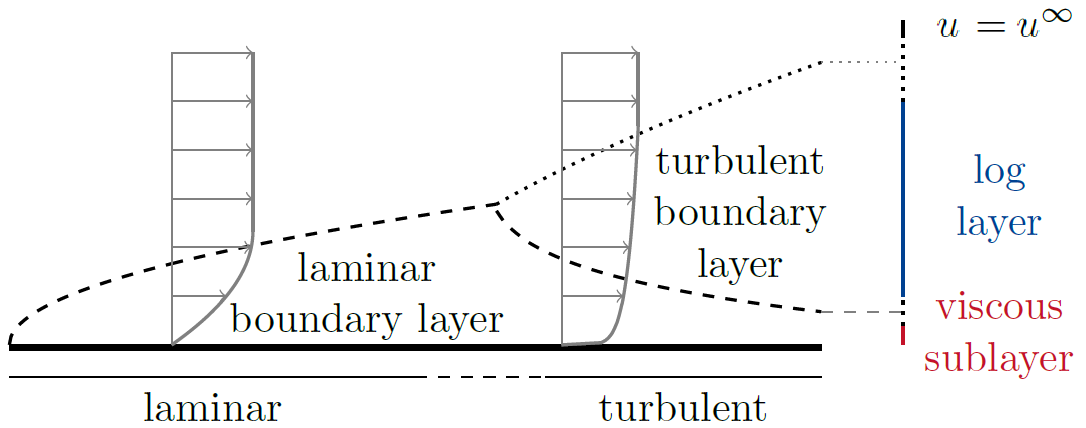
\includegraphics[width=0.8\textwidth]{boundary_layer.png}
	\caption[Boundary layer along a flat plate]{Scheme of the evolution of a 
	boundary layer along a flat plate. Figure source: \cite{tesi:fetzer}.}
	\label{fig:bl}
\end{figure}

Let us consider a flow over a flat plate as drawn in Figure~\ref{fig:bl}: when 
the flow reaches the plate a laminar boundary layer starts to develop, inside 
it a laminar regime holds and it is characterized by a moderate gradient of the 
velocity profile at the wall. After a certain distance a turbulent boundary 
layer starts to grow: it is thicker but the gradient of the velocity at the 
wall is stronger. We can define a Reynolds number based on the distance from 
the beginning of the plate and another one based on the boundary layer 
thickness:
\begin{equation}
Re_x = \frac{u^\infty x}{\nu}, \quad Re_\delta = \frac{u^\infty 
	\delta}{\nu},
\end{equation}
where $u^\infty$ is the maximum velocity far from the wall.

For the laminar boundary layer the profile can be computed analytically 
through the Blasius equation, which is obtained using dimensional arguments. 
The thickness grows as the square root of $x$:
\begin{equation}
\delta(x) = 4.9 \frac{x}{\sqrt{Re_x}} = 4.91\sqrt{\frac{x 
		\nu}{u^\infty}}.
\end{equation}
When $Re_\delta$ is higher than a certain threshold, the turbulent boundary 
layer begins, but in this case the velocity profile can be expressed only 
through some empirical laws. In order to do that it is useful to define a 
non-dimensional wall coordinate:
\begin{equation}
y^+ = \frac{u_* y}{\nu}, \quad u_* = \sqrt{\frac{\tau_w}{\varrho}},
\end{equation}
where $\tau_w$ is the shear stress at the wall. In the boundary layer four 
different regions can be identified:
\begin{itemize}
	\item near the wall, for approximately $y^+ < 5$, a small laminar viscous 
	sublayer is 
	always present and it can not be neglected. In this area the viscous 
	stresses are dominant over the Reynolds stresses and the velocity profile 
	can be approximated with a linear relation:
	\begin{equation}
	u = u_* y^+,
	\end{equation}
	\item after that there is a buffer layer in which the viscous and Reynolds 
	stresses are comparable,
	\item then, approximately in the region $30 < y^+ < 150$, there is the so 
	called log-layer, in which the velocity profile can be approximated with a 
	logarithmic function:
	\begin{equation} \label{eq:loglaw}
	u = u_* \bigg( \frac{1}{\kappa} \log y_+ + A\bigg), \quad \kappa=0.41, 
	\quad A = 
	5.5,
	\end{equation}
	where $\kappa$ is the von K\'arm\'an constant,
	\item at last there is an external region, in which the behaviour depends 
	on 
	the real situation.	
\end{itemize}
Be aware that the numbers given above as bounds for $y^+$ are not universal but 
are very problem-dependent.
\subsubsection{Turbulence models}
The quantity $\tau_R$ is a symmetric tensor with $dim \times dim$ entries, so 
in three 
dimensions we have 6 new unknowns that need to be modelled in order to close 
the problem, this procedure is known as turbulence modelling.
In 1877 Boussinesq proposed that $\tau_R$ could be similar to the viscous 
stress tensor:
\begin{equation} \label{eq:bouss}
\tau_R = 2\mu_t \bar{\mathbf{S}} - 
\frac{2}{3}\varrho k \mathbb{1}.
\end{equation}
The first term has the same form of $\tau$ if we consider the mean velocity 
field, 
the only difference is that the dynamic viscosity $\mu$ is substituted by a 
turbulent viscosity $\mu_t$ [$\si{\pascal \second}$]. The second term is needed 
to model correctly also the isotropic part of $\tau_R$, indeed:
\begin{equation} \label{eq:tracciatau}
tr(\tau_R) = -tr(\varrho \overline{\mathbf{v}' {\mathbf{v}'}^\mathrm{T}}) = 
-\varrho \sum_{i=1}^{dim} \overline{(v_i')^2} = -2\varrho k,
\end{equation}
where $k$ is the turbulent kinetic energy and it is defined as
\begin{equation}
k = \frac{1}{2} \sum_{i=1}^{dim} \overline{(v_i')^2},
\end{equation}
while exploiting equation \eqref{eq:ransmass} we get
\begin{equation}
	tr(2\mu_t \bar{S}) = 2 \mu_t \sum_{i=1}^{dim} \frac{\partial 
	\bar{v}_i}{\partial x_i} = 2\mu_t (\nabla \cdot \bar{\mathbf{v}}) = 0.
\end{equation}
With this hypothesis $\mu_t$ and $k$ are the only unknowns left and the 
momentum equation \eqref{eq:ransmom} becomes:
\begin{equation} \label{eq:ransmom2}
\frac{\partial \bar{\mathbf{v}}}{\partial t} + \nabla 
\cdot ( \bar{\mathbf{v}} \bar{\mathbf{v}}^\mathrm{T}) - \nabla \cdot 
(\nu_\text{eff} \nabla \bar{\mathbf{v}}) + \frac{1}{\varrho}\nabla (\bar{p} + 
\frac{2}{3}\varrho k) - \mathbf{g} = \mathbf{0},
\end{equation}
where we have introduced an effective kinematic viscosity
\begin{equation}
	\nu_\text{eff} = \nu + \nu_t, \quad \nu_t = \frac{\mu_t}{\varrho}.
\end{equation}
Since for incompressible fluids we have erased the thermodynamic relation 
between $\varrho$ and $p$, we can consider as unknown a generalized pressure 
$p_\text{gen}$ such that:
\begin{equation}
p_\text{gen} = \bar{p} + \frac{2}{3}\varrho k,
\end{equation}
reducing the unknowns to $\nu_t$ alone, for which we can employ different 
turbulence models to estimate it.

The idea of the Boussinesq hypothesis \eqref{eq:bouss} comes partially from an 
analogy 
between the motion 
of the turbulent structures and the molecular motion, but there are cases in 
which it can be shown that this hypothesis leads to poor results (see 
\cite{main:pope}). There exist also turbulence models called Reynolds stress 
equations models (RSM) that do not use it and try to find equations for 
all the entries of the Reynolds stress tensor, but in this way a large set of 
equations is obtained and consequently the required computational effort 
increases. See \cite{main:pope} or \cite{main:vermal} for more information.

From now on the over bar, used to denote the averaged quantities, will be 
neglected in order to simplify the notation.

\subsubsection{Zero-equations models}
The simplest turbulence models are called zero-equations models or algebraic 
models because they compute the turbulent viscosity using an algebraic relation 
that exploits geometrical quantities, so they do not introduce any additional 
PDE to the problem. Due to their simplicity they were used in the past years 
when the computational resources were limited, but they have intrinsic weak 
points because they can be applied only in special simple situations.

An important example is Prandtl's \emph{mixing length} model. It is 
useful with two-dimensional flows when the mean velocity field has a dominant 
direction and the gradient in the longitudinal direction is negligible with 
respect to that in the orthogonal direction. Let us assume that $u$ is the 
main component of the velocity and that the flow is bounded by a wall at $y=0$. 
From dimensional considerations it can be assumed that
\begin{equation}
\nu_t = = l_\text{mix}v_\text{mix},
\end{equation}
where $l_\text{mix}$ and $v_\text{mix}$ are a characteristic length scale and a 
velocity 
scale of turbulence. Then it is reasonable to chose
\begin{equation}
	v_\text{mix} = l_\text{mix} \left\lvert \frac{\partial u}{\partial y} 
	\right\rvert,
\end{equation}
because the shear stress in the mean flow gives its contribution to the 
turbulent mixing of the largest eddies. At last $l_\text{mix}$ is chosen from 
empirical considerations coming from the boundary layer theory previously 
described, for example
\begin{equation}
l_\text{mix} = \kappa y
\end{equation}
in the original version or
\begin{equation}
l_\text{mix} = \kappa y[1 - exp(y^+ / 26)]
\end{equation}
using a correction from Van Driest that dampens $\nu_t$ for $y \rightarrow 0$.
%
\subsubsection{$k\text{-}\varepsilon$ model}
Two-equation models involve the solution of two additional PDEs and the 
$k\text{-}\varepsilon$ is probably the most famous one of this category, the 
key contribution to this model was given by \textcite{turbo:ke}. It is 
based on the assumption that the turbulent viscosity $\nu_t$ could be correctly 
determined through the turbulent kinetic energy $k$ and its dissipation rate 
$\varepsilon$, so considering dimensions the relation must be
\begin{equation}
\nu_t = C_\mu \frac{k^2}{\varepsilon},
\end{equation}
where $C_\mu$ is a non-dimensional constant and $\varepsilon$ is defined as
\begin{equation}
\varepsilon = 2 \nu \overline{\mathbf{S}' \cdot \mathbf{S}'}, \quad \mathbf{S}' 
= \frac{\nabla \mathbf{v}' + (\nabla \mathbf{v}')^\mathrm{T}}{2}.
\end{equation}

Starting from the momentum equation of the Navier-Stokes model \eqref{eq:nsmom} 
and from the decomposition in mean value plus fluctuation \eqref{eq:decomp}, we 
derive an equation for $k$:
\begin{equation}
	\frac{\partial k}{\partial t} + \nabla \cdot (k\mathbf{v}) - \nabla \cdot
	\bigg[ \bigg(\nu + \frac{\nu_t}{\sigma_k}\bigg) \nabla k\bigg] 
	-2\nu_t \mathbf{S} \cdot \mathbf{S} + \varepsilon = 0,
\end{equation}
where $\sigma_k$ is a non-dimensional constant. In a similar way we could 
derive an evolution equation for $\varepsilon$, but it would contain too many 
terms difficult to model and to measure, so an empirical equation built in 
analogy with the one for $k$ is used:
\begin{equation} \label{eq:epsilon}
		\frac{\partial \varepsilon}{\partial t} + \nabla \cdot (\varepsilon 
		\mathbf{v}) - \nabla \cdot \bigg[ \bigg(\nu + 
		\frac{\nu_t}{\sigma_\varepsilon} 
		\bigg) \nabla \varepsilon \bigg] - C_{\varepsilon_1} 
		\frac{\varepsilon}{k} 2 \nu_t \mathbf{S} \cdot \mathbf{S} + 
		C_{\varepsilon_2}\frac{\varepsilon^2}{k} = 0
\end{equation}
The standard model sets the following constants:
\begin{equation}
	C_\mu = 0.09, \quad \sigma_k = 1, \quad \sigma_\varepsilon = 1.3, \quad 
	C_{\varepsilon_1} = 1.44, \quad C_{\varepsilon_2} = 1.92.
\end{equation}

This model gives its best for confined flows and high Reynolds number, where 
the Reynolds stresses are dominant. Near the wall this assumption fails, so it 
is common to use a wall function such as the one given by the boundary layer 
theory \eqref{eq:loglaw} in order to compute the velocities at the cells near 
the wall. This can be done easily for flat walls and it brings also 
computational advantages, because we can avoid to have very small cells near 
the wall that solve until the viscous sublayer.

During the years many variants of this model have been developed, for example 
the \emph{RNG}~$k\text{-}\varepsilon$ model, which is derived with a different 
procedure in order to improve the equation for
$\varepsilon$, or the \emph{low-$Re$}~$k\text{-}\varepsilon$ model, that 
adds extra terms in order to model correctly the behaviour near the wall. See 
\cite{main:vermal} for more information.
%
\subsubsection{$k\text{-}\omega$ model}
The $k\text{-}\omega$ model is another two-equations model that uses a specific 
dissipation rate $\omega$ instead of the dissipation rate $\varepsilon$; it was 
originally proposed by \textcite{komega:kolmo} and subsequently refined many 
times by \textcite{turbo:komega}.

The equation for the turbulent kinetic energy is analogous to the one used in 
the $k\text{-}\varepsilon$ model:
\begin{equation} \label{eq:komegak}
	\frac{\partial k}{\partial t} + \nabla \cdot (k\mathbf{v}) - \nabla \cdot 
\bigg[\bigg(\nu + \sigma^*\frac{k}{\omega}\bigg) \nabla k\bigg] -P + \beta^* k 
\omega = 0,
\end{equation}
with the production term $P$ that can be limited in the following way:
\begin{equation}
	P = \min \{ 2 \nu_t \mathbf{S} \cdot \mathbf{S}, 20 \beta^* k \omega \}.
\end{equation}
The equation for $\omega$ is empirical and driven by physical considerations as 
it was the equation \eqref{eq:epsilon} for $\varepsilon$:
\begin{equation} \label{eq:komegaomega}
	\frac{\partial \omega}{\partial t} + \nabla \cdot (\omega \mathbf{v}) - 
	\nabla \cdot \bigg[ \bigg( \nu + \sigma \frac{k}{\omega} \bigg) \nabla 
	\omega 
	\bigg] - \alpha \frac{\omega}{k} 2 \nu_t \mathbf{S} \cdot \mathbf{S} 
	-\frac{\sigma_d}{\omega} \nabla k \cdot 
	\nabla \omega+ \beta \omega^2 = 0
\end{equation}
The term
\begin{equation}
\frac{\sigma_d}{\omega} \nabla k \cdot \nabla \omega
\end{equation}
is new, it is related to cross-diffusion and its activation depends on the 
direction of the gradients of $k$ and $\omega$:
\begin{equation}
\sigma_d =
\begin{cases}
0 &\text{if $\nabla k \cdot \nabla \omega \leq 0$}\\
\sigma_{do} &\text{if $\nabla k \cdot \nabla \omega > 0$}
\end{cases},
\quad \sigma_{do} = \frac{1}{8}.
\end{equation}
The turbulent viscosity $\nu_t$ is obtained as
\begin{equation}
\nu_t = \frac{k}{\tilde{\omega}}, \quad \tilde{\omega} = \max \Bigg\{ \omega, 
C_\text{lim} \sqrt{ 2\frac{\mathbf{S}\cdot\mathbf{S}}{\beta^*}} \Bigg\}.
\end{equation}
The model is closed with the following coefficients:
\begin{equation}
	\beta^* = \frac{9}{100}, \quad \sigma^* = \frac{3}{5}, \quad \alpha = 
	\frac{13}{25}, \quad \beta = \frac{177}{2500}, \quad \sigma = \frac{1}{2}, 
	\quad C_\text{lim} = \frac{7}{8}.
\end{equation}

The interpretation of $\omega$ is not straight-forward: originally it was 
defined by Kolmogorov as ``the rate of dissipation of energy in unit volume and 
time'', therefore defined as
\begin{equation}
	\omega = \frac{k}{\varepsilon}.
\end{equation}
Other contributors to the development of this model have referred to it as 
the the root mean square (RMS) of the fluctuating vorticity, i.e.
\begin{equation}
	\omega = \sqrt{\overline{ (\boldsymbol\omega ')^2 }}, \quad 
	\boldsymbol\omega 
	= 
	\nabla \times \mathbf{v},
\end{equation}
in this case $\omega^2$ is the double of the \emph{enstrophy}, which is a 
quantity associated to the energy related to vorticity.

This model has shown good results also near the boundaries, so it does not 
require any wall correction. For our purposes it is the most appropriate choice 
because we would like to have non-flat boundaries, so employing a 
wall law would be cumbersome. Moreover the values near the boundary are 
very important in our tests, because they influence the exchange processes 
across the interface between free-flow and porous-medium flow.

As boundary conditions the following impositions are made:
\begin{itemize}
	\item on inflow boundaries Dirichlet conditions are set both for $k$ and 
	$\omega$. According to \cite{ko:ansys}, the following formulas can be used:
	\begin{equation} \label{eq:koic}
		k = \frac{3}{2} (|\!|\mathbf{v}|\!|_\text{in} I)^2, \quad \omega = 		
		\frac{100k^{1/2}}{7C_\mu^{1/4}L},
	\end{equation}
	where $\mathbf{v}_\text{in}$ is the inflow velocity and $I$ is a 
	non-dimensional quantity called turbulence intensity that could be 
	estimated as
	\begin{equation}
	I = \frac{0.16}{Re^{1/8}},
	\end{equation}
	$C_\mu=0.09$ and $L$ is a characteristic size of the domain,
	\item on solid walls $k=0$, while for $\omega$, according to 
	\cite{main:wilcox}, the following asymptotic behaviour is used:
	\begin{equation}
		\omega \rightarrow \frac{6 \nu}{\beta d^2} \quad \text{as} \quad d 
		\rightarrow 0,
	\end{equation}
	where $d$ is the distance from the nearest wall,
	\item on outflow and symmetry boundaries a zero-gradient condition is 
	assumed:
	\begin{equation}
		\nabla k \cdot \mathbf{n} = 0, \quad \nabla \omega \cdot \mathbf{n} = 0.
	\end{equation}
\end{itemize}
%
\section{Porous-medium flow} \label{sec:pm}
According to \cite{forch:nield} a porous-medium is ``a material consisting of a 
solid matrix with an interconnected void''. The void spaces are called 
\emph{pores} and they allow a fluid to go through the material. We consider the 
solid matrix to be fixed, neglecting the fluid-structure interaction. Examples 
of porous-media are sand, wood, soil, 
sandstone and ceramics.

In order to simulate a flow through a porous medium theoretically we could use 
the standard fluid dynamics equations at the pore scale, but this approach is 
often complex because at this level the model variables are very irregular and 
it is hard to get measurements of them. What is usually done is to 
simplify the description of the flow considering averaged quantities within a 
Representative Elementary volume (REV), thus considering the 
porous-medium as a continuum at a larger scale. In this way we lose the 
information about discontinuities at the pore scale, i.e. whether a point 
belongs to the solid matrix or is void, but we obtain more easily results that 
are comparable to experimental measurements.

Given a domain $\Omega_\text{pm}$ occupied by the porous-medium, we consider 
for every point $\mathbf{x} \in \Omega_\text{pm}$ a ball $B_r(\mathbf{x})$ of 
radius $r$, that will be the REV. Starting from a function $f$ defined at the 
pore scale we compute its average $\hat{f}$:
\begin{equation}
	\hat{f}(\mathbf{x}) = \frac{1}{|B_r(\mathbf{x})|} \int_{B_r(\mathbf{x})} 
	f(\mathbf{y}) d\mathbf{y}, \quad \forall \mathbf{x} \in \Omega_\text{pm}.
\end{equation}
The radius $r$, and thus the dimension of the REVs, should be chosen such that
\begin{equation}
	l \ll r \ll L,
\end{equation}
where $l$ is the pore scale size and $L$ is the macro scale size, as for 
example in Figure~\ref{fig:rev}. In such a way 
the high frequency variations of the microscopic properties should not be seen 
at the REV scale, but the low frequency variations of macroscopic properties 
should not be lost (see \cite{main:helmig}).
\begin{figure}
	\centering
	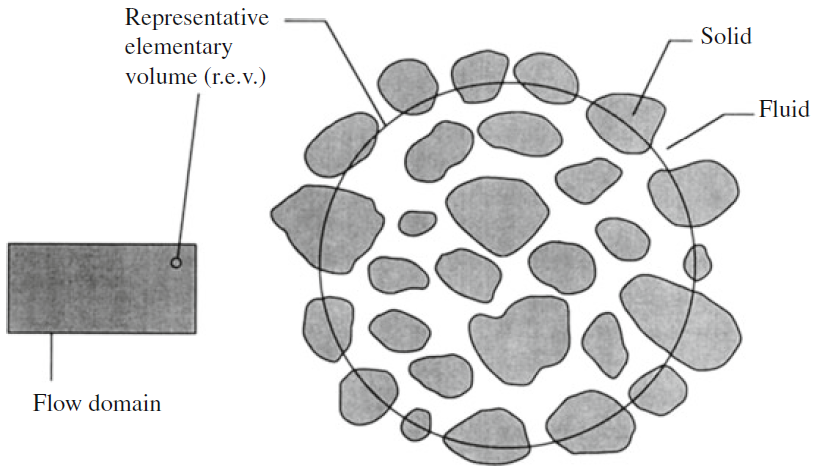
\includegraphics[width=\textwidth]{rev.png}
	\caption[REV in a porous-medium]{An example of a REV in a porous-medium. 
	Comparison of its size with the one of the pores and the one of 
	$\Omega_\text{pm}$. Figure source: \cite{forch:nield}.}
	\label{fig:rev}
\end{figure}

Let us define the \emph{porosity} of the porous-medium as
\begin{equation}
\varphi(\mathbf{x}) = \frac{1}{|B_r(\mathbf{x})|} \int_{B_r(\mathbf{x})} \chi 
(\mathbf{y}) d\mathbf{y},
\end{equation}
where $\chi(\mathbf{x})$ is the characteristic function of the void space:
\begin{equation}
\chi(\mathbf{x}) =
\begin{cases}
1 &\text{if $\mathbf{x}$ is void}\\
0 &\text{if $\mathbf{x}$ is not void}
\end{cases}, \quad \forall \mathbf{x} \in \Omega_\text{pm}.
\end{equation}

For simplicity we will assume to have porous-media with constant porosity. In 
natural materials usually $\varphi$ is not greater then $0.6$, but for some 
artificial materials, such as metallic foams, $\varphi$ could be almost $1$.
We will also consider only single-phase, single-component flows.
%
\subsection{Continuity equation}
The governing equations for a porous-medium at the REV scale can be computed 
from the standard equations for the fluid through the application of volume 
averaging techniques (see \cite{volaver:withakerbook}).

We obtain the following continuity equation:
\begin{equation}
\varphi\frac{\partial \varrho}{\partial t} + \nabla \cdot (\varrho 
\mathbf{v}) = 0,
\end{equation}
where $\varrho$ denotes the density of the fluid. $\mathbf{v}$ is the velocity 
obtained averaging over a REV containing both fluid and solid and it can be 
called \emph{Darcy} velocity or \emph{seepage} velocity. It should not be 
confused with the \emph{intrinsic} velocity $\mathbf{V}$ that we would obtain 
averaging over a REV containing only fluid, as they are related by:
\begin{equation}
	\mathbf{v} = \varphi \mathbf{V}.
\end{equation}

If we assume that the fluid is incompressible, then the continuity equation 
reduces to:
\begin{equation} \label{eq:pmcontinuity}
\nabla \cdot \mathbf{v} = 0
\end{equation}
\subsection{Momentum equation}
\subsubsection{Darcy's law}
For the momentum equation the most common choice is the Darcy's law:
\begin{equation} \label{eq:darcy}
	\mathbf{v} = -\frac{1}{\mu}\mathbf{K} (\nabla p - \varrho \mathbf{g}),
\end{equation}
where $\mathbf{K}$ [$\si{m^2}$] is the permeability tensor of the 
porous-medium; it is symmetric and positive-definite and it can be simplified 
to a scalar for isotropic porous-media. 
This equation holds for creeping flows, with $Re < 1$, for which 
inertial effect can be neglected.

It was first obtained experimentally by Henry Darcy in 1856, who discovered a 
proportionality between the flow rate and the pressure drop across a uniform 
porous-medium. After that there have been many tries to derive it analytically, 
starting from the Navier-Stokes equations and using volume averaging techniques 
with different assumptions made, see for example \cite{volaver:ithakerdarcy}. 
Moreover it can be obtained through a formal homogenization procedure if the 
porous-medium is periodic (see \cite{homo:holmes}).

The permeability is a quantity that depends only on the geometry of the porous 
medium and not on the flow, typical values range from $\SI{e-7}{m^2}$ of 
gravel to $\SI{e-16}{m^2}$ of limestone.
There are models to compute it in the case of simple geometries, for example 
through the Carman-Kozeny equation (see \cite{forch:nield}). 
%
\subsubsection{Forchheimer's law}
There exist many generalization of the Darcy's law, for example to multiphase 
and multicomponent flows, to non-Newtonian fluids or, as in this case, to 
higher Reynolds numbers. The 
extension that we are interested in is the following Forchheimer's law:
\begin{equation} \label{eq:forch}
	\mathbf{v} + C_F \sqrt{\mathbf{K}} \frac{\varrho}{\mu} 
	|\mathbf{v}|\mathbf{v} = - \frac{1}{\mu} \mathbf{K}(\nabla p - \varrho 
	\mathbf{g} ),
\end{equation}
where the second term is added to the Darcy's law in order to take into account 
also possible inertial effects. $C_F$ is a non-dimensional coefficient which is 
here taken equal to $0.55$, even if there exist many different corrections (see 
\cite{forch:nield} and \cite{forch:tesi}).

As reported by \textcite{forch:nield}, the equation was originally proposed by 
\textcite{forch:1901}, but the dependence on $\sqrt{\mathbf{K}}$ was introduced 
by \textcite{forch:ward}. \textcite{volaver:withakerforch} 
derived it with the volume averaging  starting from the Navier-Stokes equations.

This equation holds when the flow in the porous-medium is laminar, but 
the drag from linear becomes quadratic because the contribution due to solid 
obstacles becomes comparable to the one due to friction. According to 
\cite{forch:nield}, the transition from a linear to a quadratic regime is 
smooth and takes place at
\begin{equation}
	Re_\mathrm{K} \simeq 100,
\end{equation}
where $Re_\mathrm{K}$ is a Reynolds number based on the square root of the 
permeability:
\begin{equation}
	Re_\mathrm{K} = \frac{U \sqrt{\mathrm{K}}}{\nu}.
\end{equation}
%
\section{Coupling conditions} \label{sec:coupling}
At the interface between the free-flow region and the porous-medium we have to 
impose suitable conditions in order to couple the two subdomains. Let us denote 
with $\Omega_\text{ff}$ the free-flow domain and with $\Omega_\text{pm}$ the 
porous-medium domain, then
\begin{equation}
	 \Gamma_\text{int} = \overline{\Omega}_\text{ff} \cap 
	 \overline{\Omega}_\text{pm}
\end{equation}
is the interface between them.

Following \textcite{paper:mosthaf}, we would like to have conditions such that 
the interface could be as close as possible to the local thermodynamic 
equilibrium, which, however, can not be rigorously achieved because of the 
different model concepts in the two subdomains. Since we are dealing with 
single-phase, single-component isothermal flows, we only have to impose the 
mechanical equilibrium, for which we need:
\begin{itemize}
	\item the continuity of normal mass fluxes, that in our incompressible case 
	reduces to the continuity of the normal component of the velocity:
	\begin{equation} \label{eq:contmass}
		[\mathbf{v} \cdot \mathbf{n}]_\text{ff} = - [\mathbf{v} 
		\cdot \mathbf{n}]_\text{pm} \quad \text{on $\Gamma_\text{int}$},
	\end{equation}
	where the subscripts $_\text{ff}$ and $_\text{pm}$ denote that the 
	quantities are 
	evaluated in the free-flow or in the porous-medium subdomain. Notice that
	\begin{equation}
		\mathbf{n}_\text{ff} = -\mathbf{n}_\text{pm} \quad \text{on 
		$\Gamma_\text{int}$},
	\end{equation}
	\item the continuity of normal stresses:
	\begin{equation} \label{eq:coupnormalstress}
		[(\varrho \mathbf{v} \mathbf{v}^\mathrm{T} - \mu_\text{eff} \nabla 
		\mathbf{v} + p\mathbb{1}) 
		\mathbf{n}]_\text{ff} = 
		- [p\mathbf{n}]_\text{pm} \quad \text{on $\Gamma_\text{int}$},
	\end{equation}
	that may result in a jump of the pressure at the interface, even if it is 
	usually a continuous thermodynamic variable,
	\item a condition for the tangential component of the velocity in the 
	free-flow and in particular we use the one proposed by \textcite{inter:bj}:
	\begin{equation}
		\bigg[ \bigg( -\frac{\sqrt{K}}{\alpha_{BJ}} (\nabla \mathbf{v}) 
		\mathbf{n} - \mathbf{v} \bigg) \cdot \mathbf{t}_i \bigg]_\text{ff} = 
		[\mathbf{v} \cdot \mathbf{t}_i]_\text{pm}, \quad \forall i \in \{1, 
		\dots, dim - 1\},
	\end{equation}
	on $\Gamma_\text{int}$, where $\alpha_\text{BJ}$ is a non-dimensional 
	coefficient that depends on 
	properties of the permeable material and $\mathbf{t}_i, \; 
	i \in \{1, \dots, dim-1\}$ is a basis of the plane tangential to the 
	interface $\Gamma_\text{int}$. With this condition we allow a slip of the 
	tangential component of the velocity and the more the porous-medium is 
	permeable, the more slip is allowed.
	
	We also employ the simplification introduced by \textcite{inter:bjs}:
	\begin{equation}
		[\mathbf{v} \cdot \mathbf{t}_i]_\text{pm} \simeq 0, \quad \forall i \in 
		\{1, 
		\dots, dim-1\},
	\end{equation}
	so we neglect the velocity in the porous-medium since it is very small with 
	respect to the one in the free-flow region, thus obtaining the 
	Beavers-Joseph-Saffman (BJS) condition:
	\begin{equation} \label{eq:bjs}
		\bigg[ \bigg( -\frac{\sqrt{K}}{\alpha_\text{BJ}} (\nabla \mathbf{v}) 
		\mathbf{n} - \mathbf{v} \bigg) \cdot \mathbf{t}_i \bigg]_\text{ff} = 0, 
		\quad \forall i \in \{1, \dots, dim - 1\}.
	\end{equation}
\end{itemize} 
\chapter{Numerical model} \label{chap:discretization} %discretized equations?
In this chapter we describe the methods that are used to discretize the model. 
For the spatial discretization we use the finite volumes method, which allows 
to solve efficiently flow problems guaranteeing the mass conservation. See 
\cite{fv:leveque} for a broad description.
In the free-flow region we discretize the equations using the staggered grid 
concept, while in the porous-medium we employ a cell-centred approach with a 
Two Point Flux Approximation (TPFA).

For the temporal discretization we use implicit finite differences methods, 
like Backward Euler (BE) and the Backward Differencing Formula 2 (BDF2).
%
\section{Staggered grid concept}
The staggered grid concept is characterized by the distinction between the 
degrees of freedom related to scalar primary variables and those related to 
vectorial primary variables. In saddle point problems, like the incompressible 
Navier-Stokes or RANS equations, if we locate all the primary variables, i.e. 
pressure, velocity and possibly the turbulent kinetic energy and its 
dissipation rate, at the same positions in the grid, spurious modes in the 
solution may arise, leading to wrong results. A possible fix to this issue 
is thus to store the variables in a \emph{staggered} fashion, putting 
the degrees of freedom related to scalar variables at the centre of the cells 
and those related to vectorial variables on the faces, aligned to the faces 
normal direction. Therefore we obtain different control volumes, as we can see 
in Figure~\ref{fig:staggrid} for the case of the 
Navier-Stokes equations in a two-dimensional domain.
\begin{figure}[t]
	\centering
	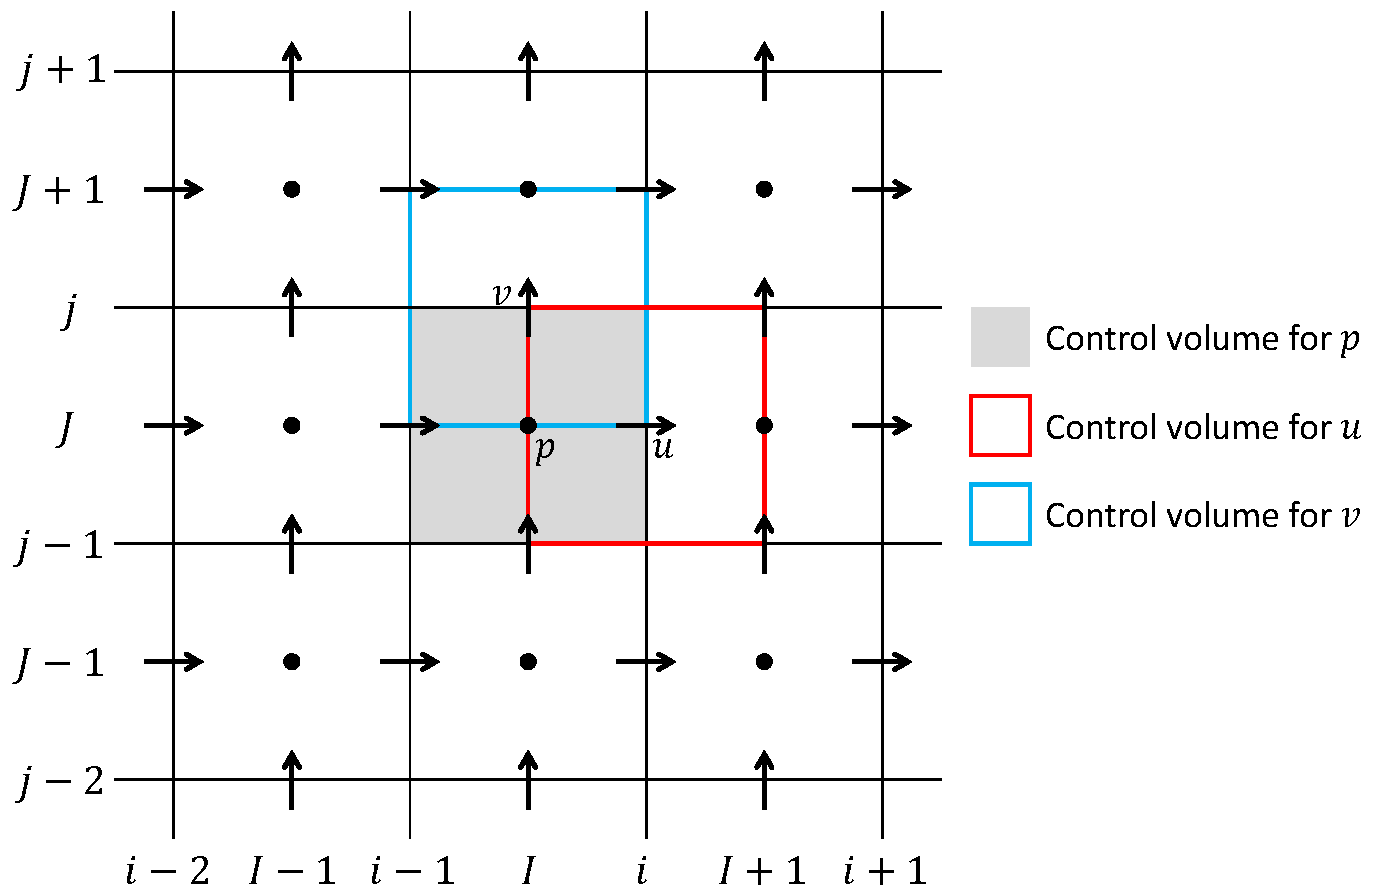
\includegraphics[width=\textwidth]{staggered_grid_mia.pdf}
	\caption[Staggered grid control volumes]{An example of a staggered grid 
	with the pressure degrees of freedom (dofs) stored at the centres of the 
	cells and the velocity dofs stored on the faces. The different control 
	volumes are highlighted. The indices in capital letters 
	$\dots,I-1,I,I+1,\dots$ 
	and $\dots,J-1,J,J+1,\dots$ refer to cells, thus to the position of 
	cell-centred variables, while the indices in lower case letters 
	$\dots,i-1,i,i+1,\dots$ and $\dots,j-1,j,j+1,\dots$ refer to faces, thus to 
	the 
	position of staggered variables.}
	\label{fig:staggrid}
\end{figure}

This approach is known also as Marker and Cell (MAC), as it was called in its 
first appearance in a paper by \textcite{stagg:orig}, within a finite 
differences framework. A more recent description can be found in 
\cite{main:vermal}.

Another advantage of this discretization method is that on the boundary we have 
the degrees of freedom of the normal component of the velocity, so it is easier 
to impose boundary and interface conditions.

For the sake of simplicity we consider now a bi-dimensional domain and 
$\mathbf{v} = [u, v]^{\mathrm{T}}$.
%
\subsection{Cell-centred equations}
\subsubsection{Continuity equation}
The continuity equation \eqref{eq:ransmass} is discretized using control 
volumes that coincide with the cells of the grid, thus it is treated is a 
cell-centred way. Since we are dealing with incompressible fluids, it does not 
involve the density and this makes its approximation easier.
%We will see in section ... how to deal with non constant desities
We integrate over the ``grey'' control 
volume $V_p = [x_{i-1},x_i] \times [y_{j-1},y_j]$, according to 
Figure~\ref{fig:staggrid}, 
and we apply the Gauss's divergence theorem:
\begin{equation}
\int_{V_p} \nabla \cdot \mathbf{v} \; dV = \int_{\partial V_p} \mathbf{v} \cdot 
\mathbf{n} \; dA = 0.
\end{equation}
The integral over the boundary $\partial V_p$ can be split over the four faces, 
that we identify with $e_p$ (east), $n_p$ (north), $w_p$ (west), $s_p$ (south):
\begin{equation}
\int_{\partial V_p} \mathbf{v} \cdot \mathbf{n} \; dA = \int_{e_p} u \; dA
+ \int_{n_p} v \; dA - \int_{w_p} u \; dA - \int_{s_p} v \; dA.
\end{equation}
At this point we discretize the equation approximating the values of the 
velocity with the values at the centre of the faces, for example:
\begin{equation}
\int_{e_p} u \; dA \approx u_{i,J} |e_p|,
\end{equation}
where $|e_p|$ denotes the measure of the face $e_p$. Thus we obtain
\begin{equation}
	u_{i,J} |e_p| + v_{I,j}|n_p| - u_{i-1,J}|w_p| - v_{I,j-1}|s_p| = 0
\end{equation}
\subsubsection{Turbulence model equations}
The equations for the turbulent kinetic energy \eqref{eq:komegak} and the 
specific dissipation rate \eqref{eq:komegaomega} are treated analogously to the 
continuity equation, but they involve more terms. Let us integrate them over 
the same control volume  $V_p = [x_{i-1},x_i] \times [y_{j-1},y_j]$:
\begin{itemize}
	\item the storage terms are approximated with the values at the centre of 
	the cell:
	\begin{equation}
	\int_{V_p} \frac{\partial k}{\partial t} \; dV = \frac{d}{dt} \int_{V_p}k 
	\; dV \approx \frac{dk_{I,J}}{dt}|V_p|,
	\end{equation}
	\begin{equation}
	\int_{V_p} \frac{\partial 
	\omega}{\partial t} \; dV = \frac{d}{dt} \int_{V_p} \omega \; dV \approx 
	\frac{\partial \omega_{I,J}}{\partial t}|V_p|.
	\end{equation}
	%
	\item the Gauss's divergence theorem is applied to the convective terms:
	\begin{equation}
		\int_{V_p} \nabla \cdot (k \mathbf{v}) \; dV = \int_{\partial V_p} k 
		(\mathbf{v} 
		\cdot \mathbf{n}) \; dA,
	\end{equation}
	\begin{equation}
	\int_{V_p} \nabla \cdot (\omega \mathbf{v}) \; dV = \int_{\partial V_p} 
	\omega 
	(\mathbf{v} \cdot \mathbf{n}) \; dA,
	\end{equation}
	then the velocity is approximated with its value at the centre of the face, 
	while for the transported quantities $k$ and $\omega$ we employ the 
	upstream value with respect to the sign of the velocity, so considering for 
	example the face $e_p$ and supposing that $u_{i,J}>0$ we have:
	\begin{equation}
		\int_{e_p} ku \; dA \approx k_{I,J}u_{i,J}|e_p|, \quad \int_{e_p} 
		\omega u \; dA \approx \omega_{I,J}u_{i,J}|e_p|.
	\end{equation}
	Notice that this approach is not the only possible choice, as it will be 
	explained with more details in Subsections~\ref{subsec:diffscheme} and 
	\ref{subsec:tvd}.
	%
	\item the Gauss's divergence theorem is applied to the diffusive terms:	
	\begin{equation}
		\int_{V_p} \nabla \cdot \bigg[\bigg(\nu + 
		\sigma^*\frac{k}{\omega}\bigg) \nabla k\bigg] \; dV = \int_{\partial 
		V_p} \bigg(\nu + \sigma^*\frac{k}{\omega}\bigg) \nabla k \cdot 
		\mathbf{n} \; dA,
	\end{equation}
	\begin{equation}
	\int_{V_p} \nabla \cdot \bigg[\bigg(\nu + \sigma\frac{k}{\omega}\bigg) 
	\nabla \omega\bigg] \; dV = \int_{\partial V_p} \bigg(\nu + \sigma 
	\frac{k}{\omega}\bigg) \nabla \omega \cdot \mathbf{n} \; dA.
	\end{equation}
	Then, considering for example the face $e_p$, the derivatives of $k$ and 
	$\omega$ are approximated with centred finite differences, while the 
	coefficients involving the viscosity are approximated by a weighted average 
	between the values at the centre of the cells sharing the face, thus 
	assuming a linear trend:
	\begin{equation}
	\int_{e_p} \bigg(\nu + \sigma^*\frac{k}{\omega}\bigg) \frac{\partial 
	k}{\partial x} \; dA \approx \bigg(\nu + \sigma^* 
	\frac{k}{\omega}\bigg)_\text{avg} \frac{k_{I+1,J}-k_{I,J}}{x_{I+1}-x_I} 
	|e_p|,
	\end{equation}
	\begin{equation}
	\int_{e_p} \bigg(\nu + \sigma\frac{k}{\omega}\bigg) \frac{\partial 
	\omega}{\partial x} \; dA \approx \bigg(\nu + \sigma 
	\frac{k}{\omega}\bigg)_\text{avg} 
	\frac{\omega_{I+1,J}-\omega_{I,J}}{x_{I+1} - x_I} |e_p|,
	\end{equation}
	where the subscript $_\text{avg}$ denotes the weighted average
	\begin{equation}
	(\ast)_\text{avg} = \frac{x_{I+1} - x_i}{x_{I+1} - x_I}(\ast)_{I,J} + 
	\frac{x_i-x_I}{x_{I+1} - x_I}(\ast)_{I+1,J}.
	\end{equation}
	%
	\item in the source terms all the quantities are approximated with their 
	value at the centre of the cell. We report here only the derivatives 
	appearing in the entries of $\mathbf{S}$, $\nabla k$ and $\nabla \omega$, 
	that are computed with centred finite differences:
	\begin{equation}
		\frac{\partial u}{\partial x}\Big|_{I,J} \approx 
		\frac{u_{i+1,J}+u_{i,J}-u_{i-1,J}-u_{i-2,J}}{2(x_{I+1}-x_{I-1})},
	\end{equation}
	\begin{equation}
	\frac{\partial v}{\partial y} \Big|_{I,J} \approx
	\frac{v_{I,j+1}+v_{I,j}-v_{I,j-1}-v_{I,j-2}}{2(y_{J+1}-y_{J-1})},
	\end{equation}
	\begin{equation}
		\frac{\partial u}{\partial y}\Big|_{I,J} \approx 
		\frac{u_{i,J+1}+u_{i-1,J+1}-u_{i,J-1}-u_{i-1,J-1}}{2(y_{J+1}-y_{J-1})},
	\end{equation}
	\begin{equation}
	\frac{\partial v}{\partial x} \Big|_{I,J} \approx 
	\frac{v_{I+1,j}+v_{I+1,j-1}-v_{I-1,j}-v_{I-1,j-1}}{2(x_{I+1}-x_{I-1})},
	\end{equation}
	\begin{equation}
		\frac{\partial k}{\partial x}\Big|_{I,J} \approx \frac{k_{I+1,J} - 
		k_{I-1,J}}{x_{I+1} - x_{I-1}}, 
		\quad \frac{\partial k}{\partial y}\Big|_{I,J} \approx 
		\frac{k_{I,J+1}-k_{i,J-1}}{y_{J+1}-y_{J-1}},
	\end{equation}
	\begin{equation}
		\frac{\partial \omega}{\partial x}\Big|_{I,J} \approx 
		\frac{\omega_{I+1,J} - \omega_{I-1,J}}{x_{I+1} - x_{I-1}}, \quad 
		\frac{\partial \omega}{\partial y}\Big|_{I,J} \approx 
		\frac{\omega_{I,J+1}-\omega_{i,J-1}}{y_{J+1}-y_{J-1}}.
	\end{equation}
	%
	\item the sink terms are approximated with the values at the centres of the 
	cells:
	\begin{equation}
		\int_{V_p} \beta^* k \omega \; dV \approx 
		\beta^*k_{I,K}\omega_{I,J}|V_p|,
	\end{equation}
	\begin{equation}
		\int_{V_p} \beta \omega^2 \; dV \approx \beta \omega_{I,J}^2 |V_p|.
	\end{equation}
\end{itemize}
%
\subsection{Staggered equations}
The momentum equation \eqref{eq:ransmom2} is discretized using the staggered 
control volumes. Let us consider the equation for the component $u$ of the 
velocity:
\begin{equation} \label{eq:stagu}
\frac{\partial u}{\partial t} + \nabla \cdot ( u \mathbf{v}) - \nabla \cdot 
(\nu_\text{eff} \nabla u) + \frac{1}{\varrho} \frac{\partial}{\partial x} 
\big(p 
+ \varrho k\big) = 0.
\end{equation}
Notice that, since we are considering a two-dimensional model, we have 
substituted the factor $2/3$ with a $1$ in front of $\varrho k$, because it 
came from the requirement \eqref{eq:tracciatau}.

We integrate it over the ``red'' control volume $V_u=[x_I, 
x_{I+1}]\times[y_{j-1},y_j]$, 
according to Figure~\ref{fig:staggrid}, and apply the Gauss's divergence 
theorem:
\begin{multline} \label{eq:stagmomeq}
\int_{V_u} \bigg[ \frac{\partial u}{\partial t} + \nabla \cdot ( u \mathbf{v} ) 
- \nabla \cdot (\nu_\text{eff} \nabla u) + \frac{1}{\varrho} 
\frac{\partial}{\partial x} \big( p + \varrho k \big) \bigg ]\; dV 
=\\
=\frac{d}{dt} \int_{V_u} u\; dV + \int_{\partial V_u} u (\mathbf{v} \cdot 
\mathbf{n}) \; dA - \int_{\partial V_u} \nu_\text{eff} (\nabla u \cdot 
\mathbf{n}) \; dA \; + \\
+\frac{1}{\varrho}\int_{\partial V_u} (p + \varrho k) n_x \; dA = 0,
\end{multline}
where $n_x$ is the component in the $x$ direction of the outward unit 
normal $\mathbf{n}$. Let us identify again the four faces of $\partial V_u$ 
with $e_u$ (east), $n_u$ (north), $w_u$ (west), $s_u$ (south), so that
\begin{equation}
	\partial V_u = e_u \cap n_u \cap w_u \cap s_u.
\end{equation}
In the equation \eqref{eq:stagmomeq} there are four terms of different nature, 
let us consider each of them separately, starting from the simplest one:
\begin{itemize}
	\item in the storage term we approximate the velocity with the value at the 
	centre of the control volume:
	\begin{equation}
	\frac{d}{dt} \int_{V_u}  u\; dV \approx \frac{du_{i,J}}{dt}|V_u|;
	\end{equation}
	%
	\item in the pressure term the contributions from the faces $n_u$ and $s_u$ 
	are null because $n_x=0$ on them, so 
	\begin{equation}
	\int_{\partial V_u} (p + \varrho k)n_x \; dA = \int_{e_u} (p+\varrho k) \; 
	dA - \int_{w_u} (p+\varrho k) \; dA.
	\end{equation}
	Then we approximate $p$ and $k$ with the values at the centre of the faces:
	\begin{equation}
	\int_{e_u} (p+\varrho k) \; dA \approx (p_{I+1,J} +\varrho k_{I+1,J}) |e_u|,
	\end{equation}
	\begin{equation}
	\int_{w_u} (p+\varrho k) \; dA \approx (p_{I,J} +\varrho k_{I,J}) |w_u|.
	\end{equation}
	%
	\item in the diffusive term we have both a frontal momentum flux 
	contribution from the faces $e_u$ and $w_u$ and a lateral momentum flux 
	contribution from the faces $n_u$ and $s_u$:
	\begin{multline}
	\int_{\partial V_u} \nu_\text{eff} (\nabla u \cdot \mathbf{n}) \; dA =     
	\int_{e_u} \nu_\text{eff} \frac{\partial u}{\partial x} \; dA
	- \int_{w_u} \nu_\text{eff} \frac{\partial u}{\partial x} \; dA \;+\\
	+\int_{n_u} \nu_\text{eff} \frac{\partial u}{\partial y} \; dA
	- \int_{s_u} \nu_\text{eff} \frac{\partial u}{\partial y} \; dA
	\end{multline}
	We develop the contributions from $e_u$ and $n_u$, the other two are 
	analogous.\\	
	For the frontal momentum flux we approximate the viscosity with 
	the value at the centre of the face, while we approximate the derivative of 
	the velocity with a centred finite difference:
	\begin{equation}
	\int_{e_u} \nu_\text{eff} \frac{\partial u}{\partial x} \; dA \approx 
	\nu_{\text{eff},\{I+1,J\}} \frac{u_{i+1,J} - u_{i,J}}{x_{i+1}-x_i} |e_u|.
	\end{equation}
	For the lateral momentum flux we split the 	face $n_u$ into the two halves 
	related to the two cells $[x_{i-1},x_i]\times[y_{j-1},y_j]$ and 
	$[x_i,x_{i+1}]\times[y_{j-1},y_j]$:
	\begin{equation}
	n_u = [x_I,x_i]\times \{y_j\} \cup [x_i,x_{I+1}] \times \{y_j\}.
	\end{equation}
	We employ again a centred finite difference to approximate the 
	derivative of the velocity, while, for the approximation of the viscosity, 
	we compute an average between the two cells sharing the face:
	\begin{equation}
	\int_{n_u} \nu_\text{eff} \frac{\partial u}{\partial y} \; dA = 
	\int_{x_{I,j}}^{x_{i,j}} \nu_\text{eff} \frac{\partial u}{\partial y} \; dA 
	+\int_{x_{i,j}}^{x_{I+1,j}} \nu_\text{eff} \frac{\partial u}{\partial y} \; 
	dA,
	\end{equation}
	\begin{equation*}
	\int_{x_{I,j}}^{x_{i,j}} \nu_\text{eff} \frac{\partial u}{\partial y} \; dA 
	\approx \frac{1}{2}\big(\nu_{\text{eff},\{I,J\}}+\nu_{\text{eff},\{I,J+1\}} 
	\big) \frac{u_{i,J+1}-u_{i,J}}{y_{J+1}-y_J} \frac{|n_u|}{2},
	\end{equation*}
	\begin{equation*}
	\int_{x_{i,j}}^{x_{I+1,j}} \nu_\text{eff} \frac{\partial u}{\partial y} \; 
	dA \approx \frac{1}{2}\big( \nu_{\text{eff},\{I+1,J\}}+ 
	\nu_{\text{eff},\{I+1,J+1\}} \big) \frac{u_{i,J+1}-u_{i,J}}{y_{J+1}-y_J} 
	\frac{|n_u|}{2}.
	\end{equation*}
	%
	\item in the convective term we have again both a frontal momentum flux 
	contribution from the faces $e_u$ and $w_u$ and a lateral momentum flux 
	contribution from the faces $n_u$ and $s_u$:
	\begin{multline}
	\int_{\partial V_u} u (\mathbf{v} \cdot \mathbf{n}) \; dA = \int_{e_u} u u 
	\; dA - \int_{w_u} u u \; dA \; +\\
	+ \int_{n_u} u v \; dA  -\int_{s_u} u v \; dA.
	\end{multline}
	For the discretization we have to distinguish between the 
	\emph{transporting velocity}, coming from $\mathbf{v} \cdot \mathbf{n}$, 
	and the \emph{transported field}, that in this case is the velocity itself. 
	For the former we average between the values sharing the face, 
	while for the latter we have to consider an approximation that takes into 
	account the flow direction, as it will be explained in detail in 
	Subsections~\ref{subsec:diffscheme} and \ref{subsec:tvd}. For the moment we 
	simply denote this approximation with a superscript $^*$.
	We develop only the contributions from $e_u$ and $n_u$, the other two are 
	analogous.\\
	For the frontal momentum flux we approximate the transporting velocity with 
	an average between the values at the centre of the two staggered cells 
	sharing the staggered face:
	\begin{equation}
		\int_{e_u} u u \; dA \approx u^* \frac{u_{i,J} + 
		u_{i+1,J}}{2}|e_u|.
	\end{equation}
	For the lateral momentum flux we approximate the transporting velocity with 
	an average between the values a the two ends of the face (see 
	Figure~\ref{fig:lat_adv_flux}):
	\begin{equation}
	\int_{n_u} u v \; dA \approx u^* \frac{v_{I,j} 
	+v_{I+1,j}}{2} |n_u|.
	\end{equation}
	\begin{figure}
		\centering
		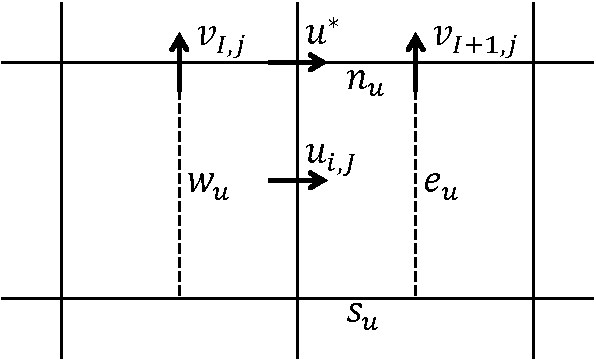
\includegraphics[width=0.6\textwidth]{lateral_adv_flux_black.pdf}
		\caption[Degrees of freedom involved in the lateral part of the 
		advective flux]{Degrees of freedom involved in the lateral part of the 
		advective flux.}
		\label{fig:lat_adv_flux}
	\end{figure}
\end{itemize}
The equation for the component $v$ of the velocity is analogous to the one for 
$u$ described above, with the only addition of the gravity term:
\begin{equation}
\frac{\partial v}{\partial t} + \nabla \cdot (v \mathbf{v}) - \nabla \cdot 
(\nu_\text{eff} \nabla v) + \frac{1}{\varrho}\frac{\partial}{\partial y} \big(p 
+ \varrho k\big) - g= 0,
\end{equation}
with $g = \SI{-9.81}{m/s}$. The gravity term is discretized straight-forward:
\begin{equation}
\int_{V_v} g \; dV = g |V_v|,
\end{equation}
where $V_v = [x_{i-1}, xi] \times [y_J, y_{J+1}]$ is the ``blue'' control 
volume in 
Figure~\ref{fig:staggrid}. 

%
\subsection{Differencing schemes} \label{subsec:diffscheme} %Linear 
%differencing schemes ?
The choice of the scheme for the approximation of a transported field is of 
great importance for both the accuracy and the stability of the solution of the 
problem. In general this decision has to be taken for every convective term, 
indeed we have found it both in the discretization of the velocity 
equation and of the turbulence model equations. As already mentioned, an 
important property that the scheme should have is the \emph{transportativeness} 
(see \cite{main:vermal}), i.e. it should take into account the direction of the 
flow. From a physical point of view this comes from the fact that, when in a 
flow convection is dominating over diffusion, a bias of the value on the face 
towards the direction where the flow comes from must occur. From a mathematical 
point of view instead we can introduce the following \emph{Péclet number}
\begin{equation}
	Pe = \frac{|u| h}{2\nu},
\end{equation}
where $h$ denotes the cell width. When the grid is too coarse or the viscosity 
is too low $Pe\rightarrow\infty$, and this can lead to a lost of stability of 
the numerical method (see for example \cite{main:quarteroni}).

In the following we will list the most immediate options, referring to the 
convective term of the equation~\eqref{eq:stagu} for the $x$-component of the 
velocity. It is considered here the case of a uniform grid, with positive 
transporting velocity according to 
Figure~\ref{fig:superscripts}, but all the schemes can be generalized to the 
case of non-uniform grids. Moreover the basic construction is one-dimensional, 
so it can be used for every dimension also in a multi-dimensional problem. For 
a complete description see for example in \cite{main:vermal}.
\begin{figure}
	\centering
	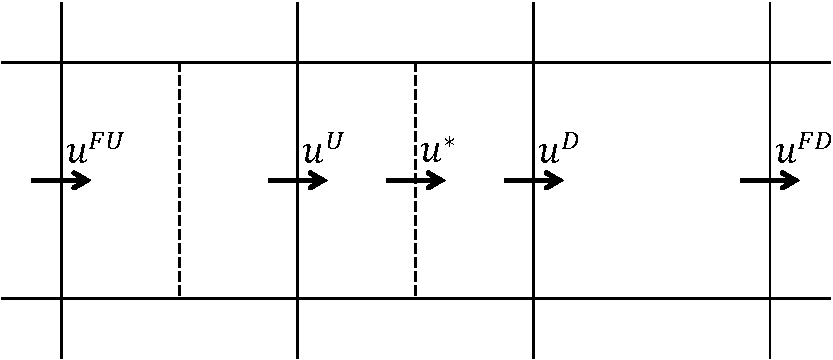
\includegraphics[width=0.75\textwidth]{trecelle_black.pdf}
	\caption[Location of the degrees of freedom used to approximate 
	$u^*$]{Location of the degrees of freedom used to approximate $u^*$. The 
	superscripts $^U$, $^{FU}$, $^D$ and $^{FD}$ stand respectively for 
	upstream, far-upstream, downstream and far-downstream. They hold for the 
	case of positive transporting velocity at the face where $u^*$ is.}
	\label{fig:superscripts}
\end{figure}
\subsubsection{CD scheme}
The Central Differencing (CD) scheme consists in using an average between the 
two first neighbouring values:
\begin{equation} \label{eq:cd}
	u^* = \frac{u^D + u^U}{2}.
\end{equation}
Employing Taylor expansions, it can be easily seen that this approximation is 
of second order, but being symmetric it does not have the transportativeness 
property. Indeed it can be shown that when $Pe > 1$ it is not stable.
%
\subsubsection{Upwind scheme}
In opposition to the CD scheme, the upwind scheme consists in using only the 
upstream value:
\begin{equation}
	u^* = u^U
\end{equation}
It is a simple, widely used and robust scheme as it has the transportativeness 
property, but its accuracy is only of first order, indeed it introduces in the 
solution an important amount of numerical diffusion that smooths the gradients. 
%
\subsubsection{Hybrid scheme}
The hybrid scheme (\cite{diff:hybrid}) consists in evaluating if $Pe<1$ or 
$Pe>1$ at each face and then employing the CD or the upwind respectively. It 
exploits the good properties of the two schemes mentioned above, so it is 
highly stable and accurate when the diffusion is dominant, however the overall 
accuracy in terms of Taylor expansions reduces to first order.
%
\subsubsection{QUICK scheme}
The Quadratic Upstream Interpolation for Convective Kinetics (QUICK) scheme 
(\cite{fv:leonard}) is an higher-order method that involves an extended stencil 
of degrees of freedom. It can be obtained evaluating the quadratic interpolator 
of $u^D$, $u^U$ and 
$u^{FU}$ at the position where $u^*$ is:
\begin{equation} \label{eq:quick}
	u^* = \frac{3u^D + 6u^U - u^{FU}}{8}.
\end{equation}
Its accuracy is of third order, but it may produce unphysical overshoots or 
undershoots in the solution when there are strong gradients. This behaviour is 
not desirable, in particular in the case where the simulation involves 
quantities such as the turbulent kinetic energy $k$ that have to be positive. 
%
\subsubsection{LUD scheme}
The Linear Upwind Differencing (LUD) scheme is an extension of the upwind 
scheme that has a second order accuracy, however it can produce too unphysical 
oscillations. It can be obtained evaluating the linear interpolator of $u^U$ 
and 
$u^{FU}$ at the position where $u^*$ is:
\begin{equation} \label{eq:lud}
u^* = \frac{3u^U - u^{FU}}{2}
\end{equation}
%
\subsubsection{An example}
We can see the behaviour of the CD, Upwind and QUICK methods when they are 
applied to a one-dimensional scalar conservation law:
\begin{align}
	\label{eq:1dconslaw} \frac{\partial \phi}{\partial t} + \frac{\partial 
	\phi}{\partial x} = 0, 
	\quad &\forall x \in (0, 1), \; \forall t > 0\\
	\phi(0, t) = 1, \quad &\forall t>0\\
	\label{eq:1dconslawend}\phi(x, 0) = 0, \quad &\forall x \in (0,1)
\end{align}
In this case there is no diffusion but only the linear transport of a step from 
left to right. The equation~\eqref{eq:1dconslaw} can be discretized with finite 
volumes storing the degrees of freedom at the ends of each cells, as it is in 
the staggered grid concept. Then the differencing schemes presented above can 
be applied to the discretization of the transport term, while for the temporal 
discretization we can use the Backward Euler method (see 
Subsection~\ref{subsec:time}).
\begin{figure}[t]
	\centering
	% This file was created by matlab2tikz.
%
\definecolor{mycolor1}{rgb}{0.00000,0.44700,0.74100}%
\definecolor{mycolor2}{rgb}{0.85000,0.32500,0.09800}%
\definecolor{mycolor3}{rgb}{0.92900,0.69400,0.12500}%
\definecolor{mycolor4}{rgb}{0.49400,0.18400,0.55600}%
%
\begin{tikzpicture}

\begin{axis}[%
width=4.521in,
height=3.566in,
at={(0.758in,0.481in)},
scale only axis,
xmin=0,
xmax=1,
xlabel={$x$},
ymin=-0.2,
ymax=1.2,
ylabel style={rotate=-90},
ylabel={$\phi$},
axis background/.style={fill=white},
xmajorgrids,
ymajorgrids,
legend style={legend cell align=left, align=left}
]
\addplot [color=mycolor1, line width=1.0pt]
  table[row sep=crcr]{%
0	1\\
0.01	0.999999999999998\\
0.02	0.999999999999996\\
0.03	0.999999999999994\\
0.04	0.999999999999992\\
0.05	0.999999999999989\\
0.06	0.999999999999986\\
0.07	0.99999999999996\\
0.08	0.999999999999793\\
0.09	0.999999999998831\\
0.1	0.999999999993898\\
0.11	0.999999999971067\\
0.12	0.999999999874841\\
0.13	0.999999999502328\\
0.14	0.999999998168577\\
0.15	0.999999993725629\\
0.16	0.999999979885173\\
0.17	0.999999939386113\\
0.18	0.999999827634698\\
0.19	0.999999535839338\\
0.2	0.999998812633614\\
0.21	0.999997106525567\\
0.22	0.999993265936024\\
0.23	0.999984997559364\\
0.24	0.999967937904754\\
0.25	0.999934141695054\\
0.26	0.999869744553662\\
0.27	0.999751533017892\\
0.28	0.999542175213802\\
0.29	0.999183955854206\\
0.3	0.998591041052117\\
0.31	0.997640580657252\\
0.32	0.996163325498081\\
0.33	0.993934852516489\\
0.34	0.990668881094432\\
0.35	0.986014435190807\\
0.36	0.979558658275129\\
0.37	0.970836838452181\\
0.38	0.959350608906481\\
0.39	0.944594376212604\\
0.4	0.926088890922847\\
0.41	0.903419671442894\\
0.42	0.876276925280645\\
0.43	0.844492887025716\\
0.44	0.808072276594065\\
0.45	0.767211963651117\\
0.46	0.722306892457252\\
0.47	0.673940758463859\\
0.48	0.622861630494047\\
0.49	0.569944427843504\\
0.5	0.516143635538314\\
0.51	0.462440662855497\\
0.52	0.409790689637048\\
0.53	0.359073669980816\\
0.54	0.311053438676802\\
0.55	0.266347735122728\\
0.56	0.225410611537675\\
0.57	0.188527326489454\\
0.58	0.15582061757907\\
0.59	0.12726632782502\\
0.6	0.102715798267608\\
0.61	0.0819222436879219\\
0.62	0.064568457451522\\
0.63	0.050293568773193\\
0.64	0.0387171078248224\\
0.65	0.0294592278334407\\
0.66	0.0221565085115676\\
0.67	0.0164732627583193\\
0.68	0.0121086534010078\\
0.69	0.00880018614753774\\
0.7	0.00632428443479598\\
0.71	0.00449468953278292\\
0.72	0.00315938979635853\\
0.73	0.00219669263790105\\
0.74	0.00151093575790394\\
0.75	0.00102821009176346\\
0.76	0.000692350052533607\\
0.77	0.000461345838948479\\
0.78	0.000304252064420694\\
0.79	0.000198607416515645\\
0.8	0.000128339745066717\\
0.81	8.21068112383886e-05\\
0.82	5.20112987575462e-05\\
0.83	3.26260518048084e-05\\
0.84	2.02687530901388e-05\\
0.85	1.24718860439782e-05\\
0.86	7.60197122584152e-06\\
0.87	4.5904488488754e-06\\
0.88	2.74640275388882e-06\\
0.89	1.62816405785874e-06\\
0.9	9.56535504982658e-07\\
0.91	5.5695043665537e-07\\
0.92	3.21430766012914e-07\\
0.93	1.83889140173297e-07\\
0.94	1.04295159237761e-07\\
0.95	5.86479341944607e-08\\
0.96	3.27010904856373e-08\\
0.97	1.80814200246999e-08\\
0.98	9.91523108869357e-09\\
0.99	5.3927683848014e-09\\
1	3.78657525181429e-09\\
};
\addlegendentry{Upwind}

\addplot [color=mycolor2, line width=1.0pt]
  table[row sep=crcr]{%
0	1\\
0.01	0.999965710272451\\
0.02	1.0003711465264\\
0.03	1.00014854307904\\
0.04	0.999270844467522\\
0.05	0.99960061856003\\
0.06	1.00102346309916\\
0.07	1.00086577735392\\
0.08	0.99886995603546\\
0.09	0.998429046767205\\
0.1	1.00083403493599\\
0.11	1.00239038375991\\
0.12	1.00012095987893\\
0.13	0.997070624727386\\
0.14	0.998159339376732\\
0.15	1.00247724177743\\
0.16	1.00390489753821\\
0.17	0.999721043584093\\
0.18	0.995016751203348\\
0.19	0.996388693579341\\
0.2	1.00305748718819\\
0.21	1.0070996420994\\
0.22	1.00283795879653\\
0.23	0.994077686119459\\
0.24	0.990516376643465\\
0.25	0.99720788995073\\
0.26	1.00856755910146\\
0.27	1.01330322516727\\
0.28	1.00533865198346\\
0.29	0.990143473793654\\
0.3	0.980639837378823\\
0.31	0.986428547191385\\
0.32	1.0055054295642\\
0.33	1.02499426078756\\
0.34	1.03002123275231\\
0.35	1.01405329869804\\
0.36	0.98370328084332\\
0.37	0.955361373773731\\
0.38	0.946290123037388\\
0.39	0.965579669516141\\
0.4	1.0095677179787\\
0.41	1.06328348178933\\
0.42	1.10635367292669\\
0.43	1.12018661001756\\
0.44	1.09346505650795\\
0.45	1.0243789005889\\
0.46	0.919640397126949\\
0.47	0.791419977970305\\
0.48	0.65367119674773\\
0.49	0.519030386095064\\
0.5	0.396908803611655\\
0.51	0.292845366943997\\
0.52	0.208828815737963\\
0.53	0.144163960111455\\
0.54	0.0964932311582958\\
0.55	0.0627076139101309\\
0.56	0.0396176304571858\\
0.57	0.0243623166423223\\
0.58	0.0145977859589567\\
0.59	0.00853165663445841\\
0.6	0.00486815225843776\\
0.61	0.00271428768884109\\
0.62	0.0014799878436374\\
0.63	0.000789762153221659\\
0.64	0.000412737425771835\\
0.65	0.000211385129457051\\
0.66	0.000106160712960325\\
0.67	5.23108205197296e-05\\
0.68	2.53041786042231e-05\\
0.69	1.20222887601928e-05\\
0.7	5.6128716363789e-06\\
0.71	2.57622411591923e-06\\
0.72	1.16297368003659e-06\\
0.73	5.16560761864122e-07\\
0.74	2.25843172929901e-07\\
0.75	9.72270535293513e-08\\
0.76	4.12301492874685e-08\\
0.77	1.72280576588568e-08\\
0.78	7.09562783110579e-09\\
0.79	2.88145498743889e-09\\
0.8	1.15405650598619e-09\\
0.81	4.55993814246403e-10\\
0.82	1.77797204740791e-10\\
0.83	6.84286241215848e-11\\
0.84	2.60019559804264e-11\\
0.85	9.75739490100953e-12\\
0.86	3.616777968438e-12\\
0.87	1.32454500734859e-12\\
0.88	4.79360068971018e-13\\
0.89	1.71473634698169e-13\\
0.9	6.06401463557598e-14\\
0.91	2.12048214707643e-14\\
0.92	7.33334019249338e-15\\
0.93	2.50865286932442e-15\\
0.94	8.49038192920412e-16\\
0.95	2.84337363183936e-16\\
0.96	9.42429903646218e-17\\
0.97	3.09084521166096e-17\\
0.98	1.00693670408514e-17\\
0.99	3.14077517289222e-18\\
1	1.30466238536566e-18\\
};
\addlegendentry{CD}

\addplot [color=mycolor3, line width=1.0pt]
  table[row sep=crcr]{%
0	1\\
0.01	0.999999999995262\\
0.02	1.00000000004294\\
0.03	0.9999999999912\\
0.04	0.99999999978397\\
0.05	1.00000000007817\\
0.06	1.00000000078217\\
0.07	0.999999999738437\\
0.08	0.999999997478595\\
0.09	1.00000000044043\\
0.1	1.00000000758953\\
0.11	1.00000000077066\\
0.12	0.999999978722831\\
0.13	0.999999989546124\\
0.14	1.00000005365586\\
0.15	1.00000005558989\\
0.16	0.999999888198641\\
0.17	0.999999783023942\\
0.18	1.00000014365421\\
0.19	1.00000066917569\\
0.2	1.00000016879789\\
0.21	0.999998441135465\\
0.22	0.999998136214366\\
0.23	1.00000208086011\\
0.24	1.00000680693682\\
0.25	1.00000234725487\\
0.26	0.999986008302737\\
0.27	0.999977192386767\\
0.28	1.00000468433908\\
0.29	1.0000611995447\\
0.3	1.00007464548147\\
0.31	0.999963804672798\\
0.32	0.999768474427161\\
0.33	0.999717492876302\\
0.34	1.0000740864123\\
0.35	1.00078152688761\\
0.36	1.00121594040801\\
0.37	1.00044548221478\\
0.38	0.998081689000521\\
0.39	0.995224889179441\\
0.4	0.994620035501864\\
0.41	0.999393171277525\\
0.42	1.01062375269566\\
0.43	1.02497613745603\\
0.44	1.03394302606178\\
0.45	1.02559975158592\\
0.46	0.988454410759239\\
0.47	0.915793052889107\\
0.48	0.808577592237637\\
0.49	0.675636328584134\\
0.5	0.531162002238621\\
0.51	0.390681264237169\\
0.52	0.267129177339398\\
0.53	0.168344132852575\\
0.54	0.0964975297312753\\
0.55	0.0491554716101291\\
0.56	0.0211897918605249\\
0.57	0.00671289177835233\\
0.58	0.000482493061530729\\
0.59	-0.0014066429442749\\
0.6	-0.00143498240798926\\
0.61	-0.000929732816774027\\
0.62	-0.000455118195225722\\
0.63	-0.000161407874156621\\
0.64	-2.54614459088232e-05\\
0.65	1.75654911986119e-05\\
0.66	2.03641743786821e-05\\
0.67	1.23082448611261e-05\\
0.68	5.110132501568e-06\\
0.69	1.23558886770601e-06\\
0.7	-1.68399632307439e-07\\
0.71	-3.89521164225457e-07\\
0.72	-2.51907941517708e-07\\
0.73	-1.02706380241783e-07\\
0.74	-2.24857631892333e-08\\
0.75	4.57658242611726e-09\\
0.76	7.56691986686351e-09\\
0.77	4.29278769841257e-09\\
0.78	1.46170982216117e-09\\
0.79	1.72039443552797e-10\\
0.8	-1.55346555440935e-10\\
0.81	-1.31647173167267e-10\\
0.82	-5.64411371340995e-11\\
0.83	-1.24899207153375e-11\\
0.84	1.9906596373481e-12\\
0.85	3.35824693909456e-12\\
0.86	1.70700405002962e-12\\
0.87	4.67687981928616e-13\\
0.88	-2.23227565065507e-15\\
0.89	-7.70766789518374e-14\\
0.9	-4.44186596934674e-14\\
0.91	-1.33448697541153e-14\\
0.92	-6.52923800100817e-16\\
0.93	1.69069287314303e-15\\
0.94	1.0405244781143e-15\\
0.95	3.18554261065671e-16\\
0.96	1.87786792697895e-17\\
0.97	-3.6768924328292e-17\\
0.98	-2.23805157994266e-17\\
0.99	-6.58055008490752e-18\\
1	-4.00561578240812e-19\\
};
\addlegendentry{QUICK}

\addplot [color=mycolor4, line width=1.0pt]
  table[row sep=crcr]{%
0	1\\
0.5	1\\
0.5	0\\
1	0\\
};
\addlegendentry{Exact}

\end{axis}
\end{tikzpicture}%
	\caption[Solution of a one-dimensional scalar conservation law]{Solution of 
	the problem \eqref{eq:1dconslaw}--\eqref{eq:1dconslawend} at the time 
	$t=0.5$. The upwind method smooths the gradient, while the CD and QUICK 
	methods produce oscillations.}
	\label{fig:1dconslaw}
\end{figure}

In Figure~\ref{fig:1dconslaw} we can see the solution at $t=0.5$. The upwind 
method is very diffusive near the step, but bounded within the extrema of the 
exact solution. The CD and QUICK methods instead approximate better the steep 
gradient, but produce oscillations for $x<0.5$.
%
\subsection{TVD methods} \label{subsec:tvd}
Total Variation Diminishing (TVD) methods belong to a category of methods 
called \emph{high resolution methods}, that address the problem of computing a 
solution without any oscillation and with an higher order accuracy, second 
order in this case. They were originally developed for scalar conservation laws 
of the type:
\begin{align}
	\label{eq:conslaw} &\frac{\partial \phi}{\partial t} + \frac{\partial f(x) 
	}{\partial x} = 0. 
%\quad t>0 \quad x 
%	\in 
%	\mathbb{R}\\[1ex]
%	\label{eq:conslawic} &\phi(x, 0) = \phi_0(x), \quad x \in \mathbb{R}
\end{align}

For this kind of problems the \emph{total variation} of the numerical solution 
can be defined as:
\begin{equation}
	TV(\phi) = \sum_{i=1}^{N_\text{dof}-1} |\phi_{i+1} - \phi_i|,
\end{equation}
where $\phi_i$ is the numerical solution at the node $i$ of the discretized 
domain. A method is called TVD if the total variation of the 
solution does not increase with time: 
\begin{equation}\label{eq:tvdcondition}
	TV(\phi ^{n+1}) \leq TV(\phi^n) \quad \forall n>0,
\end{equation}
where $\phi^n$ is the numerical solution at the time-step $t^n$. In 
\cite{tvd:monotonicity} it has been proved that a TVD scheme is 
\emph{monotonicity preserving}, i.e. it does not create new 
local extrema, local minima are non-decreasing and local maxima are 
non-increasing. This is the desirable property that we would like to have in 
order avoid the creation of solutions containing overshoots and undershoots, 
as it happens using the higher order methods presented in the previous 
subsection.

According to \cite{tvd:sweeby} and \cite{main:darwish} we can achieve our 
target adding to the first order upwind approximation a second order 
non-linear 
anti-diffusive flux: 
\begin{equation} \label{eq:tvdformula}
u^* = u^U + \frac{1}{2}\psi(r)(u^D - u^U), \quad r = 
\frac{u^U - u^{FU}}{u^D - u^U}.
\end{equation}
The flux includes a function $\psi$ called \emph{flux limiter}, indeed it 
should dampen the flux contribution in regions of the domain where it 
could produce oscillations. It is chosen non-negative in order to preserve the 
sign of the flux and it depends on the variable $r$, that is defined as the 
ratio between two consecutive differences of the solution. The non-linearity 
can not be avoided, indeed it was proved by \textcite{tvd:godunov} that any 
monotonicity preserving linear scheme can be at most first order accurate.

Exploiting the approximation \eqref{eq:tvdformula} to solve a problem like
\eqref{eq:conslaw} and imposing the TVD condition \eqref{eq:tvdcondition} on 
the solution, we obtain the following bounds for the flux limiter function:
\begin{align}
\notag \psi(r) = 0 \quad &\text{if} \quad r < 0\\
\psi(r) \leq \min \{2r, 1\} \quad &\text{if} \quad 0 \leq r \leq 1\\
\notag \psi(r) \leq 2 \quad &\text{if} \quad r > 2
\end{align}
Notice that when $r<0$ we are in presence of a local maximum or minimum, 
because it means that the differences between the upstream and downstream nodes 
and the one between the far upstream and upstream nodes have opposite signs. 
When this happens, $\psi$ is set to zero, so only the first order upwind 
contribution is employed in the approximation of $u^*$.
It is also required to $\psi$ to fulfil the following symmetry property:
\begin{equation}
\frac{\psi(r)}{r} = \psi\bigg(\frac{1}{r}\bigg),
\end{equation}
which ensures that backward- and forward-facing gradients are treated in the 
same way.

In order to have a second order scheme, $\psi$ must be at least 
Lipschitz-continuous. Moreover, following \cite{tvd:sweeby} and 
\cite{tvd:vanleer}, any second order scheme 
can be obtained as a convex combination of the CD scheme \eqref{eq:cd} and the 
LUD scheme \eqref{eq:lud}, in the following way:
\begin{equation}
	\psi(r) = \theta(r) \psi_{CD}(r) + (1-\theta(r))\psi_{LUD}(r) \quad \forall 
	r >0,
\end{equation}
where $\theta(r)$ is a parameter such that $0 \leq \theta(r) \leq 1,\; \forall 
r>0$, while $\psi_{CD}$ and $\psi_{LUD}$ are the linear flux limiter functions 
that can be associated to the schemes CD and LUD rearranging the 
approximations \eqref{eq:cd} and \eqref{eq:lud}:
\begin{gather}
	\psi_{CD}(r) = 1 \quad \forall r,\\
	\psi_{LUD}(r) = r \quad \forall r.
\end{gather}
Thus, adding these requirements to the previous ones, we 
obtain the following bounds for the flux limiter function of a TVD method:
\begin{align}
\psi(r) = 0 \quad &\text{if} \quad r < 0 \notag \\
\label{eq:tvdbounds} r \leq \psi(r) \leq \min \{2r, 1\} \quad &\text{if} \quad 
0 
\leq r \leq 1\\
1 \leq \psi(r) \leq \min \{r, 2 \} \quad &\text{if} \quad r > 2 \notag
\end{align}
In Figure~\ref{fig:tvdregion} they are reported in a $\psi-r$ diagram known 
also as Sweby's diagram.
\begin{figure}
	\centering
	% This file was created by matlab2tikz.
%
\begin{tikzpicture}

\begin{axis}[%
width=0.951\widthsette,
height=0.68\widthsette,
scale only axis,
xmin=0,
xmax=3.5,
xlabel style={font=\color{white!15!black}},
xlabel={$r$},
ymin=0,
ymax=2.5,
ylabel style={font=\color{white!15!black}, rotate=-90},
ylabel={$\psi$},
axis background/.style={fill=white},
xmajorgrids,
ymajorgrids,
]

\addplot[area legend, draw=black, fill=white!80!black, fill opacity=0.5, forget plot, line width=1pt]
table[row sep=crcr] {%
x	y\\
0	0\\
1	1\\
0.5	1\\
}--cycle;

\addplot[area legend, draw=black, fill=white!80!black, fill opacity=0.5, forget plot, line width=1pt]
table[row sep=crcr] {%
x	y\\
1	1\\
5.5	1\\
5.5	2\\
2	2\\
}--cycle;

\end{axis}
\end{tikzpicture}%
	\caption[TVD region (Sweby's diagram)]{In grey the TVD region in which 
	the flux 
	limiter functions must fit. It is called also Sweby's diagram.}
	\label{fig:tvdregion}
\end{figure}
% A livello teorico potrei aggiungere la dimostrazione di monotonicity->TVD, 
%l'applicazione di TVD per ottenere i bounds e l'applicazione dei bounds 
%all'approssimazione col flux limiter (come in sweby o in darwish). Potrei 
%mettere qualcosa nell'appendice.
\subsubsection{Flux limters}
Starting from the bounds \eqref{eq:tvdbounds}, it is easy to create a 
flux limiter function, indeed in literature many possible choices can be 
found. 
We list here some of the most popular functions that have been implemented in 
\DUMUX and in Figure~\ref{fig:fluxlimiters} we can see their graph in the 
Sweby's diagram:
\begin{itemize}
	\item Van Leer \cite{tvd:vanleer}
	\begin{equation} \label{eq:vl}
	\psi(r) = \frac{r+|r|}{1+r}.
	\end{equation}
	It is a smooth function that asymptotically reaches 2 for $r \rightarrow 
	\infty$.
%
	\item Van Alabada \cite{tvd:vanalabada}
	\begin{equation} \label{eq:vanalabada}
	\psi(r)=
	\begin{cases}
	\dfrac{r^2+r}{r^2+1} \quad &\text{if $r\geq 0$}\\[2ex]
	0 \quad &\text{if $r<0$}
	\end{cases}
	\end{equation}
	It is a smooth function that instead goes to 1 as $r \rightarrow \infty$.
%
	\item Min-Mod \cite{tvd:roe}
	\begin{equation} \label{eq:minmod}
	\psi(r) = \max \{0, \min \{ r,1\} \}
	\end{equation}
	It is a piecewise linear function that lies on the lower boundary of the 
	TVD region. Intuitively, using this limiter we add to the upstream value  
	half of	the smallest increment in absolute value between $u^U-u^{FU}$ and 
	$u^D - u^U$.
%
	\item Superbee \cite{tvd:roe}
	\begin{equation} \label{eq:superbee}
	\psi(r)=\max \{0, \min \{ 2r, 1\}, \min \{ r, 2\} \}
	\end{equation}
	It is a piecewise linear function that lies on the upper boundary of the 
	TVD region.
%
	\item UMIST \cite{tvd:lien}
	\begin{equation} \label{eq:umist}
	\psi(r)=\max \bigg\{0, \min \bigg\{ 2r, \frac{3r+1}{4},\frac{r+3}{4}, 
	2\bigg\} \bigg\}
	\end{equation}
	It is a piecewise linear function that was designed as a symmetrical TVD 
	version of QUICK.
%
	\item MC (Monotinized Central) limiter \cite{tvd:mclimiter}
	\begin{equation} \label{eq:mclim}
	\psi(r)=\max \bigg\{0, \min \bigg\{ 2r, \frac{r+1}{2}, 2\bigg\} \bigg\}
	\end{equation}
	It is also known as MUSCL (Monotonic Upstream-Centred Scheme for 
	Conservation Laws) limiter.
%	
%	\item WAHYD \cite{nonunif:hou}
%	\begin{equation}
%	\psi(r)=
%	\begin{cases}
%	\dfrac{r + |r|}{r + 1} & \text{if $r \leq 1$} \\[2ex]
%	\min \bigg\{ \dfrac{r + 2 r^2}{2 + r^2}, 2 \bigg\} & \text{if $r>1$}
%	\end{cases}
%	\end{equation}
%	It is a hybrid scheme, for $r\leq 1$ it is the Van Leer scheme 
%	\eqref{eq:vl}, while for $r>1$ it is closer to the upper bound of the TVD 
%	region.
\end{itemize}
\begin{figure}[t]
	\centering
	% This file was created by matlab2tikz.
%
\definecolor{mycolor1}{rgb}{0.92900,0.69400,0.12500}%
\definecolor{mycolor2}{rgb}{0.49400,0.18400,0.55600}%
\definecolor{mycolor3}{rgb}{0.46600,0.67400,0.18800}%
\definecolor{mycolor4}{rgb}{0.30100,0.74500,0.93300}%
\definecolor{mycolor5}{rgb}{0.63500,0.07800,0.18400}%
\definecolor{mycolor6}{rgb}{0.00000,0.44700,0.74100}%
%
\begin{tikzpicture}

\begin{axis}[%
width=4.521in,
height=3.566in,
at={(0.758in,0.481in)},
scale only axis,
xmin=0,
xmax=5.5,
xlabel={$r$},
ymin=0,
ymax=3,
ylabel style={rotate=-90},
ylabel={$\psi$},
axis background/.style={fill=white},
xmajorgrids,
ymajorgrids,
legend style={at={(0.03,0.97)}, anchor=north west, legend cell align=left, align=left}
]

\addplot[area legend, draw=none, fill=white!95!black, fill opacity=0.5, forget plot]
table[row sep=crcr] {%
x	y\\
0	0\\
1	1\\
0.5	1\\
}--cycle;

\addplot[area legend, draw=none, fill=white!95!black, fill opacity=0.5, forget plot]
table[row sep=crcr] {%
x	y\\
1	1\\
5.5	1\\
5.5	2\\
2	2\\
}--cycle;
\addplot [color=mycolor1, line width=1.0pt]
  table[row sep=crcr]{%
0	0\\
0.05	0.0952380952380952\\
0.1	0.181818181818182\\
0.15	0.260869565217391\\
0.2	0.333333333333333\\
0.25	0.4\\
0.3	0.461538461538462\\
0.35	0.518518518518518\\
0.4	0.571428571428572\\
0.45	0.620689655172414\\
0.5	0.666666666666667\\
0.55	0.709677419354839\\
0.6	0.75\\
0.65	0.787878787878788\\
0.7	0.823529411764706\\
0.75	0.857142857142857\\
0.8	0.888888888888889\\
0.85	0.918918918918919\\
0.9	0.947368421052632\\
0.95	0.974358974358974\\
1	1\\
1.05	1.02439024390244\\
1.1	1.04761904761905\\
1.15	1.06976744186047\\
1.2	1.09090909090909\\
1.25	1.11111111111111\\
1.3	1.1304347826087\\
1.35	1.14893617021277\\
1.4	1.16666666666667\\
1.45	1.18367346938776\\
1.5	1.2\\
1.55	1.2156862745098\\
1.6	1.23076923076923\\
1.65	1.24528301886792\\
1.7	1.25925925925926\\
1.75	1.27272727272727\\
1.8	1.28571428571429\\
1.85	1.29824561403509\\
1.9	1.31034482758621\\
1.95	1.32203389830508\\
2	1.33333333333333\\
2.05	1.34426229508197\\
2.1	1.35483870967742\\
2.15	1.36507936507937\\
2.2	1.375\\
2.25	1.38461538461538\\
2.3	1.39393939393939\\
2.35	1.40298507462687\\
2.4	1.41176470588235\\
2.45	1.42028985507246\\
2.5	1.42857142857143\\
2.55	1.43661971830986\\
2.6	1.44444444444444\\
2.65	1.45205479452055\\
2.7	1.45945945945946\\
2.75	1.46666666666667\\
2.8	1.47368421052632\\
2.85	1.48051948051948\\
2.9	1.48717948717949\\
2.95	1.49367088607595\\
3	1.5\\
3.05	1.50617283950617\\
3.1	1.51219512195122\\
3.15	1.51807228915663\\
3.2	1.52380952380952\\
3.25	1.52941176470588\\
3.3	1.53488372093023\\
3.35	1.54022988505747\\
3.4	1.54545454545455\\
3.45	1.55056179775281\\
3.5	1.55555555555556\\
3.55	1.56043956043956\\
3.6	1.56521739130435\\
3.65	1.56989247311828\\
3.7	1.57446808510638\\
3.75	1.57894736842105\\
3.8	1.58333333333333\\
3.85	1.58762886597938\\
3.9	1.59183673469388\\
3.95	1.5959595959596\\
4	1.6\\
4.05	1.6039603960396\\
4.1	1.6078431372549\\
4.15	1.61165048543689\\
4.2	1.61538461538462\\
4.25	1.61904761904762\\
4.3	1.62264150943396\\
4.35	1.62616822429907\\
4.4	1.62962962962963\\
4.45	1.63302752293578\\
4.5	1.63636363636364\\
4.55	1.63963963963964\\
4.6	1.64285714285714\\
4.65	1.64601769911504\\
4.7	1.64912280701754\\
4.75	1.65217391304348\\
4.8	1.6551724137931\\
4.85	1.65811965811966\\
4.9	1.66101694915254\\
4.95	1.66386554621849\\
5	1.66666666666667\\
5.05	1.66942148760331\\
5.1	1.67213114754098\\
5.15	1.67479674796748\\
5.2	1.67741935483871\\
5.25	1.68\\
5.3	1.68253968253968\\
5.35	1.68503937007874\\
5.4	1.6875\\
5.45	1.68992248062016\\
5.5	1.69230769230769\\
};
\addlegendentry{Van Leer}

\addplot [color=mycolor2, line width=1.0pt]
  table[row sep=crcr]{%
0	0\\
0.05	0.0523690773067332\\
0.1	0.108910891089109\\
0.15	0.168704156479218\\
0.2	0.230769230769231\\
0.25	0.294117647058824\\
0.3	0.357798165137615\\
0.35	0.420935412026726\\
0.4	0.482758620689655\\
0.45	0.542619542619542\\
0.5	0.6\\
0.55	0.654510556621881\\
0.6	0.705882352941177\\
0.65	0.753954305799649\\
0.7	0.798657718120805\\
0.75	0.84\\
0.8	0.878048780487805\\
0.85	0.912917271407838\\
0.9	0.94475138121547\\
0.95	0.973718791064389\\
1	1\\
1.05	1.02378121284185\\
1.1	1.04524886877828\\
1.15	1.06458557588805\\
1.2	1.08196721311475\\
1.25	1.09756097560976\\
1.3	1.11152416356877\\
1.35	1.12400354295837\\
1.4	1.13513513513514\\
1.45	1.1450443190975\\
1.5	1.15384615384615\\
1.55	1.16164584864071\\
1.6	1.1685393258427\\
1.65	1.17461383478845\\
1.7	1.17994858611825\\
1.75	1.18461538461538\\
1.8	1.18867924528302\\
1.85	1.19219898247598\\
1.9	1.19522776572668\\
1.95	1.19781363872983\\
2	1.2\\
2.05	1.20182604517059\\
2.1	1.20332717190388\\
2.15	1.20453534904402\\
2.2	1.20547945205479\\
2.25	1.20618556701031\\
2.3	1.20667726550079\\
2.35	1.20697585281717\\
2.4	1.20710059171598\\
2.45	1.20706890396287\\
2.5	1.20689655172414\\
2.55	1.20659780073309\\
2.6	1.20618556701031\\
2.65	1.20567154876909\\
2.7	1.20506634499397\\
2.75	1.2043795620438\\
2.8	1.20361990950226\\
2.85	1.20279528637983\\
2.9	1.201912858661\\
2.95	1.20097912909044\\
3	1.2\\
3.05	1.19898082989566\\
3.1	1.19792648444863\\
3.15	1.19684138246738\\
3.2	1.19572953736655\\
3.25	1.19459459459459\\
3.3	1.19343986543314\\
3.35	1.19226835753733\\
3.4	1.19108280254777\\
3.45	1.18988568106956\\
3.5	1.18867924528302\\
3.55	1.1874655394229\\
3.6	1.18624641833811\\
3.65	1.18502356432187\\
3.7	1.18379850238257\\
3.75	1.18257261410788\\
3.8	1.18134715025907\\
3.85	1.18012324221836\\
3.9	1.17890191239975\\
3.95	1.17768408372233\\
4	1.17647058823529\\
4.05	1.17526217497486\\
4.1	1.17405951712521\\
4.15	1.1728632185485\\
4.2	1.17167381974249\\
4.25	1.17049180327869\\
4.3	1.1693175987686\\
4.35	1.16815158740118\\
4.4	1.16699410609037\\
4.45	1.16584545126788\\
4.5	1.16470588235294\\
4.55	1.163575624928\\
4.6	1.16245487364621\\
4.65	1.16134379489446\\
4.7	1.16024252923343\\
4.75	1.15915119363395\\
4.8	1.15806988352745\\
4.85	1.15699867468651\\
4.9	1.15593762495002\\
4.95	1.15488677580629\\
5	1.15384615384615\\
5.05	1.15281577209697\\
5.1	1.15179563124769\\
5.15	1.15078572077391\\
5.2	1.14978601997147\\
5.25	1.14879649890591\\
5.3	1.14781711928498\\
5.35	1.14684783526036\\
5.4	1.14588859416446\\
5.45	1.14493933718753\\
5.5	1.144\\
};
\addlegendentry{Van Alabada}

\addplot [color=mycolor3, line width=1.0pt]
  table[row sep=crcr]{%
0	0\\
0.05	0.05\\
0.1	0.1\\
0.15	0.15\\
0.2	0.2\\
0.25	0.25\\
0.3	0.3\\
0.35	0.35\\
0.4	0.4\\
0.45	0.45\\
0.5	0.5\\
0.55	0.55\\
0.6	0.6\\
0.65	0.65\\
0.7	0.7\\
0.75	0.75\\
0.8	0.8\\
0.85	0.85\\
0.9	0.9\\
0.95	0.95\\
1	1\\
1.05	1\\
1.1	1\\
1.15	1\\
1.2	1\\
1.25	1\\
1.3	1\\
1.35	1\\
1.4	1\\
1.45	1\\
1.5	1\\
1.55	1\\
1.6	1\\
1.65	1\\
1.7	1\\
1.75	1\\
1.8	1\\
1.85	1\\
1.9	1\\
1.95	1\\
2	1\\
2.05	1\\
2.1	1\\
2.15	1\\
2.2	1\\
2.25	1\\
2.3	1\\
2.35	1\\
2.4	1\\
2.45	1\\
2.5	1\\
2.55	1\\
2.6	1\\
2.65	1\\
2.7	1\\
2.75	1\\
2.8	1\\
2.85	1\\
2.9	1\\
2.95	1\\
3	1\\
3.05	1\\
3.1	1\\
3.15	1\\
3.2	1\\
3.25	1\\
3.3	1\\
3.35	1\\
3.4	1\\
3.45	1\\
3.5	1\\
3.55	1\\
3.6	1\\
3.65	1\\
3.7	1\\
3.75	1\\
3.8	1\\
3.85	1\\
3.9	1\\
3.95	1\\
4	1\\
4.05	1\\
4.1	1\\
4.15	1\\
4.2	1\\
4.25	1\\
4.3	1\\
4.35	1\\
4.4	1\\
4.45	1\\
4.5	1\\
4.55	1\\
4.6	1\\
4.65	1\\
4.7	1\\
4.75	1\\
4.8	1\\
4.85	1\\
4.9	1\\
4.95	1\\
5	1\\
5.05	1\\
5.1	1\\
5.15	1\\
5.2	1\\
5.25	1\\
5.3	1\\
5.35	1\\
5.4	1\\
5.45	1\\
5.5	1\\
};
\addlegendentry{Min-Mod}

\addplot [color=mycolor4, line width=1.0pt]
  table[row sep=crcr]{%
0	0\\
0.05	0.1\\
0.1	0.2\\
0.15	0.3\\
0.2	0.4\\
0.25	0.5\\
0.3	0.6\\
0.35	0.7\\
0.4	0.8\\
0.45	0.9\\
0.5	1\\
0.55	1\\
0.6	1\\
0.65	1\\
0.7	1\\
0.75	1\\
0.8	1\\
0.85	1\\
0.9	1\\
0.95	1\\
1	1\\
1.05	1.05\\
1.1	1.1\\
1.15	1.15\\
1.2	1.2\\
1.25	1.25\\
1.3	1.3\\
1.35	1.35\\
1.4	1.4\\
1.45	1.45\\
1.5	1.5\\
1.55	1.55\\
1.6	1.6\\
1.65	1.65\\
1.7	1.7\\
1.75	1.75\\
1.8	1.8\\
1.85	1.85\\
1.9	1.9\\
1.95	1.95\\
2	2\\
2.05	2\\
2.1	2\\
2.15	2\\
2.2	2\\
2.25	2\\
2.3	2\\
2.35	2\\
2.4	2\\
2.45	2\\
2.5	2\\
2.55	2\\
2.6	2\\
2.65	2\\
2.7	2\\
2.75	2\\
2.8	2\\
2.85	2\\
2.9	2\\
2.95	2\\
3	2\\
3.05	2\\
3.1	2\\
3.15	2\\
3.2	2\\
3.25	2\\
3.3	2\\
3.35	2\\
3.4	2\\
3.45	2\\
3.5	2\\
3.55	2\\
3.6	2\\
3.65	2\\
3.7	2\\
3.75	2\\
3.8	2\\
3.85	2\\
3.9	2\\
3.95	2\\
4	2\\
4.05	2\\
4.1	2\\
4.15	2\\
4.2	2\\
4.25	2\\
4.3	2\\
4.35	2\\
4.4	2\\
4.45	2\\
4.5	2\\
4.55	2\\
4.6	2\\
4.65	2\\
4.7	2\\
4.75	2\\
4.8	2\\
4.85	2\\
4.9	2\\
4.95	2\\
5	2\\
5.05	2\\
5.1	2\\
5.15	2\\
5.2	2\\
5.25	2\\
5.3	2\\
5.35	2\\
5.4	2\\
5.45	2\\
5.5	2\\
};
\addlegendentry{Superbee}

\addplot [color=mycolor5, line width=1.0pt]
  table[row sep=crcr]{%
0	0\\
0.05	0.1\\
0.1	0.2\\
0.15	0.3\\
0.2	0.4\\
0.25	0.5\\
0.3	0.6\\
0.35	0.675\\
0.4	0.7\\
0.45	0.725\\
0.5	0.75\\
0.55	0.775\\
0.6	0.8\\
0.65	0.825\\
0.7	0.85\\
0.75	0.875\\
0.8	0.9\\
0.85	0.925\\
0.9	0.95\\
0.95	0.975\\
1	1\\
1.05	1.025\\
1.1	1.05\\
1.15	1.075\\
1.2	1.1\\
1.25	1.125\\
1.3	1.15\\
1.35	1.175\\
1.4	1.2\\
1.45	1.225\\
1.5	1.25\\
1.55	1.275\\
1.6	1.3\\
1.65	1.325\\
1.7	1.35\\
1.75	1.375\\
1.8	1.4\\
1.85	1.425\\
1.9	1.45\\
1.95	1.475\\
2	1.5\\
2.05	1.525\\
2.1	1.55\\
2.15	1.575\\
2.2	1.6\\
2.25	1.625\\
2.3	1.65\\
2.35	1.675\\
2.4	1.7\\
2.45	1.725\\
2.5	1.75\\
2.55	1.775\\
2.6	1.8\\
2.65	1.825\\
2.7	1.85\\
2.75	1.875\\
2.8	1.9\\
2.85	1.925\\
2.9	1.95\\
2.95	1.975\\
3	2\\
3.05	2\\
3.1	2\\
3.15	2\\
3.2	2\\
3.25	2\\
3.3	2\\
3.35	2\\
3.4	2\\
3.45	2\\
3.5	2\\
3.55	2\\
3.6	2\\
3.65	2\\
3.7	2\\
3.75	2\\
3.8	2\\
3.85	2\\
3.9	2\\
3.95	2\\
4	2\\
4.05	2\\
4.1	2\\
4.15	2\\
4.2	2\\
4.25	2\\
4.3	2\\
4.35	2\\
4.4	2\\
4.45	2\\
4.5	2\\
4.55	2\\
4.6	2\\
4.65	2\\
4.7	2\\
4.75	2\\
4.8	2\\
4.85	2\\
4.9	2\\
4.95	2\\
5	2\\
5.05	2\\
5.1	2\\
5.15	2\\
5.2	2\\
5.25	2\\
5.3	2\\
5.35	2\\
5.4	2\\
5.45	2\\
5.5	2\\
};
\addlegendentry{MC Limiter}

\addplot [color=mycolor6, line width=1.0pt]
  table[row sep=crcr]{%
0	0\\
0.05	0.1\\
0.1	0.2\\
0.15	0.3\\
0.2	0.4\\
0.25	0.4375\\
0.3	0.475\\
0.35	0.5125\\
0.4	0.55\\
0.45	0.5875\\
0.5	0.625\\
0.55	0.6625\\
0.6	0.7\\
0.65	0.7375\\
0.7	0.775\\
0.75	0.8125\\
0.8	0.85\\
0.85	0.8875\\
0.9	0.925\\
0.95	0.9625\\
1	1\\
1.05	1.0125\\
1.1	1.025\\
1.15	1.0375\\
1.2	1.05\\
1.25	1.0625\\
1.3	1.075\\
1.35	1.0875\\
1.4	1.1\\
1.45	1.1125\\
1.5	1.125\\
1.55	1.1375\\
1.6	1.15\\
1.65	1.1625\\
1.7	1.175\\
1.75	1.1875\\
1.8	1.2\\
1.85	1.2125\\
1.9	1.225\\
1.95	1.2375\\
2	1.25\\
2.05	1.2625\\
2.1	1.275\\
2.15	1.2875\\
2.2	1.3\\
2.25	1.3125\\
2.3	1.325\\
2.35	1.3375\\
2.4	1.35\\
2.45	1.3625\\
2.5	1.375\\
2.55	1.3875\\
2.6	1.4\\
2.65	1.4125\\
2.7	1.425\\
2.75	1.4375\\
2.8	1.45\\
2.85	1.4625\\
2.9	1.475\\
2.95	1.4875\\
3	1.5\\
3.05	1.5125\\
3.1	1.525\\
3.15	1.5375\\
3.2	1.55\\
3.25	1.5625\\
3.3	1.575\\
3.35	1.5875\\
3.4	1.6\\
3.45	1.6125\\
3.5	1.625\\
3.55	1.6375\\
3.6	1.65\\
3.65	1.6625\\
3.7	1.675\\
3.75	1.6875\\
3.8	1.7\\
3.85	1.7125\\
3.9	1.725\\
3.95	1.7375\\
4	1.75\\
4.05	1.7625\\
4.1	1.775\\
4.15	1.7875\\
4.2	1.8\\
4.25	1.8125\\
4.3	1.825\\
4.35	1.8375\\
4.4	1.85\\
4.45	1.8625\\
4.5	1.875\\
4.55	1.8875\\
4.6	1.9\\
4.65	1.9125\\
4.7	1.925\\
4.75	1.9375\\
4.8	1.95\\
4.85	1.9625\\
4.9	1.975\\
4.95	1.9875\\
5	2\\
5.05	2\\
5.1	2\\
5.15	2\\
5.2	2\\
5.25	2\\
5.3	2\\
5.35	2\\
5.4	2\\
5.45	2\\
5.5	2\\
};
\addlegendentry{UMIST}

\end{axis}
\end{tikzpicture}%
	\caption[Flux limiter functions]{The Sweby's diagram with the flux limiters 
	presented in this section as functions of $r$.}
	\label{fig:fluxlimiters}
\end{figure}

It is not easy to compare the different flux limiters in order to find the 
best one. Generally the Van Alabada and the Min-Mod can be a bit less accurate 
since $\psi \rightarrow 1$ as $r \rightarrow \infty$, while a scheme like the 
Superbee can produce sharper gradients, but sometimes the convergence can be a 
bit more difficult (it is said to be too compressive). The UMIST instead has a 
more complex function, so its evaluation can be more expensive. However their 
performances should be compared case by case.

In Figure~\ref{fig:1dconslawtvd} we can see the application of the TVD method 
using the Van Leer flux limiter \eqref{eq:quick:vl} to the problem 
\eqref{eq:1dconslaw}--\eqref{eq:1dconslawend}. It can be observed that the 
gradient is approximated with the same accuracy of the QUICK scheme 
\eqref{eq:quick}, but the overshoot for $x<0.5$ is avoided.
\begin{figure}
	\centering
	% This file was created by matlab2tikz.
%
\definecolor{mycolor1}{rgb}{0.00000,0.44700,0.74100}%
\definecolor{mycolor2}{rgb}{0.85000,0.32500,0.09800}%
\definecolor{mycolor3}{rgb}{0.92900,0.69400,0.12500}%
\definecolor{mycolor4}{rgb}{0.49400,0.18400,0.55600}%
%
\begin{tikzpicture}

\begin{axis}[%
width=4.521in,
height=3.566in,
at={(0.758in,0.481in)},
scale only axis,
xmin=0,
xmax=1,
xlabel style={font=\color{white!15!black}},
xlabel={$x$},
ymin=-0.2,
ymax=1.2,
ylabel style={font=\color{white!15!black}, rotate=-90},
ylabel={$\phi$},
axis background/.style={fill=white},
xmajorgrids,
ymajorgrids,
legend style={legend cell align=left, align=left, draw=white!15!black}
]
\addplot [color=mycolor1, line width=1.0pt]
  table[row sep=crcr]{%
0	1\\
0.01	0.999999999999998\\
0.02	0.999999999999996\\
0.03	0.999999999999994\\
0.04	0.999999999999992\\
0.05	0.999999999999989\\
0.06	0.999999999999986\\
0.07	0.99999999999996\\
0.08	0.999999999999793\\
0.09	0.999999999998831\\
0.1	0.999999999993898\\
0.11	0.999999999971067\\
0.12	0.999999999874841\\
0.13	0.999999999502328\\
0.14	0.999999998168577\\
0.15	0.999999993725629\\
0.16	0.999999979885173\\
0.17	0.999999939386113\\
0.18	0.999999827634698\\
0.19	0.999999535839338\\
0.2	0.999998812633614\\
0.21	0.999997106525567\\
0.22	0.999993265936024\\
0.23	0.999984997559364\\
0.24	0.999967937904754\\
0.25	0.999934141695054\\
0.26	0.999869744553662\\
0.27	0.999751533017892\\
0.28	0.999542175213802\\
0.29	0.999183955854206\\
0.3	0.998591041052117\\
0.31	0.997640580657252\\
0.32	0.996163325498081\\
0.33	0.993934852516489\\
0.34	0.990668881094432\\
0.35	0.986014435190807\\
0.36	0.979558658275129\\
0.37	0.970836838452181\\
0.38	0.959350608906481\\
0.39	0.944594376212604\\
0.4	0.926088890922847\\
0.41	0.903419671442894\\
0.42	0.876276925280645\\
0.43	0.844492887025716\\
0.44	0.808072276594065\\
0.45	0.767211963651117\\
0.46	0.722306892457252\\
0.47	0.673940758463859\\
0.48	0.622861630494047\\
0.49	0.569944427843504\\
0.5	0.516143635538314\\
0.51	0.462440662855497\\
0.52	0.409790689637048\\
0.53	0.359073669980816\\
0.54	0.311053438676802\\
0.55	0.266347735122728\\
0.56	0.225410611537675\\
0.57	0.188527326489454\\
0.58	0.15582061757907\\
0.59	0.12726632782502\\
0.6	0.102715798267608\\
0.61	0.0819222436879219\\
0.62	0.064568457451522\\
0.63	0.050293568773193\\
0.64	0.0387171078248224\\
0.65	0.0294592278334407\\
0.66	0.0221565085115676\\
0.67	0.0164732627583193\\
0.68	0.0121086534010078\\
0.69	0.00880018614753774\\
0.7	0.00632428443479598\\
0.71	0.00449468953278292\\
0.72	0.00315938979635853\\
0.73	0.00219669263790105\\
0.74	0.00151093575790394\\
0.75	0.00102821009176346\\
0.76	0.000692350052533607\\
0.77	0.000461345838948479\\
0.78	0.000304252064420694\\
0.79	0.000198607416515645\\
0.8	0.000128339745066717\\
0.81	8.21068112383886e-05\\
0.82	5.20112987575462e-05\\
0.83	3.26260518048084e-05\\
0.84	2.02687530901388e-05\\
0.85	1.24718860439782e-05\\
0.86	7.60197122584152e-06\\
0.87	4.5904488488754e-06\\
0.88	2.74640275388882e-06\\
0.89	1.62816405785874e-06\\
0.9	9.56535504982658e-07\\
0.91	5.5695043665537e-07\\
0.92	3.21430766012914e-07\\
0.93	1.83889140173297e-07\\
0.94	1.04295159237761e-07\\
0.95	5.86479341944607e-08\\
0.96	3.27010904856373e-08\\
0.97	1.80814200246999e-08\\
0.98	9.91523108869357e-09\\
0.99	5.3927683848014e-09\\
1	3.78657525181429e-09\\
};
\addlegendentry{Upwind}

\addplot [color=mycolor3, line width=1.0pt]
  table[row sep=crcr]{%
0	1\\
0.01	0.999999999995262\\
0.02	1.00000000004294\\
0.03	0.9999999999912\\
0.04	0.99999999978397\\
0.05	1.00000000007817\\
0.06	1.00000000078217\\
0.07	0.999999999738437\\
0.08	0.999999997478595\\
0.09	1.00000000044043\\
0.1	1.00000000758953\\
0.11	1.00000000077066\\
0.12	0.999999978722831\\
0.13	0.999999989546124\\
0.14	1.00000005365586\\
0.15	1.00000005558989\\
0.16	0.999999888198641\\
0.17	0.999999783023942\\
0.18	1.00000014365421\\
0.19	1.00000066917569\\
0.2	1.00000016879789\\
0.21	0.999998441135465\\
0.22	0.999998136214366\\
0.23	1.00000208086011\\
0.24	1.00000680693682\\
0.25	1.00000234725487\\
0.26	0.999986008302737\\
0.27	0.999977192386767\\
0.28	1.00000468433908\\
0.29	1.0000611995447\\
0.3	1.00007464548147\\
0.31	0.999963804672798\\
0.32	0.999768474427161\\
0.33	0.999717492876302\\
0.34	1.0000740864123\\
0.35	1.00078152688761\\
0.36	1.00121594040801\\
0.37	1.00044548221478\\
0.38	0.998081689000521\\
0.39	0.995224889179441\\
0.4	0.994620035501864\\
0.41	0.999393171277525\\
0.42	1.01062375269566\\
0.43	1.02497613745603\\
0.44	1.03394302606178\\
0.45	1.02559975158592\\
0.46	0.988454410759239\\
0.47	0.915793052889107\\
0.48	0.808577592237637\\
0.49	0.675636328584134\\
0.5	0.531162002238621\\
0.51	0.390681264237169\\
0.52	0.267129177339398\\
0.53	0.168344132852575\\
0.54	0.0964975297312753\\
0.55	0.0491554716101291\\
0.56	0.0211897918605249\\
0.57	0.00671289177835233\\
0.58	0.000482493061530729\\
0.59	-0.0014066429442749\\
0.6	-0.00143498240798926\\
0.61	-0.000929732816774027\\
0.62	-0.000455118195225722\\
0.63	-0.000161407874156621\\
0.64	-2.54614459088232e-05\\
0.65	1.75654911986119e-05\\
0.66	2.03641743786821e-05\\
0.67	1.23082448611261e-05\\
0.68	5.110132501568e-06\\
0.69	1.23558886770601e-06\\
0.7	-1.68399632307439e-07\\
0.71	-3.89521164225457e-07\\
0.72	-2.51907941517708e-07\\
0.73	-1.02706380241783e-07\\
0.74	-2.24857631892333e-08\\
0.75	4.57658242611726e-09\\
0.76	7.56691986686351e-09\\
0.77	4.29278769841257e-09\\
0.78	1.46170982216117e-09\\
0.79	1.72039443552797e-10\\
0.8	-1.55346555440935e-10\\
0.81	-1.31647173167267e-10\\
0.82	-5.64411371340995e-11\\
0.83	-1.24899207153375e-11\\
0.84	1.9906596373481e-12\\
0.85	3.35824693909456e-12\\
0.86	1.70700405002962e-12\\
0.87	4.67687981928616e-13\\
0.88	-2.23227565065507e-15\\
0.89	-7.70766789518374e-14\\
0.9	-4.44186596934674e-14\\
0.91	-1.33448697541153e-14\\
0.92	-6.52923800100817e-16\\
0.93	1.69069287314303e-15\\
0.94	1.0405244781143e-15\\
0.95	3.18554261065671e-16\\
0.96	1.87786792697895e-17\\
0.97	-3.6768924328292e-17\\
0.98	-2.23805157994266e-17\\
0.99	-6.58055008490752e-18\\
1	-4.00561578240812e-19\\
};
\addlegendentry{QUICK}

\addplot [color=mycolor2, line width=1.0pt]
  table[row sep=crcr]{%
0	1\\
0.01	0.999999999999999\\
0.02	0.999999999999997\\
0.03	0.999999999999995\\
0.04	0.999999999999993\\
0.05	0.999999999999991\\
0.06	0.999999999999988\\
0.07	0.999999999999986\\
0.08	0.999999999999984\\
0.09	0.999999999999982\\
0.1	0.99999999999998\\
0.11	0.999999999999977\\
0.12	0.999999999999975\\
0.13	0.999999999999973\\
0.14	0.999999999999971\\
0.15	0.999999999999968\\
0.16	0.999999999999962\\
0.17	0.999999999999936\\
0.18	0.999999999999856\\
0.19	0.999999999999619\\
0.2	0.999999999998931\\
0.21	0.999999999996951\\
0.22	0.999999999991255\\
0.23	0.999999999974869\\
0.24	0.999999999927722\\
0.25	0.999999999792065\\
0.26	0.999999999401777\\
0.27	0.999999998278902\\
0.28	0.999999995047466\\
0.29	0.999999985742021\\
0.3	0.999999958924243\\
0.31	0.999999881617694\\
0.32	0.999999659094588\\
0.33	0.999999021500203\\
0.34	0.999997211005141\\
0.35	0.999992143488204\\
0.36	0.999978244023689\\
0.37	0.999941103133325\\
0.38	0.999844960323749\\
0.39	0.999605120742507\\
0.4	0.999031311945721\\
0.41	0.997720625947108\\
0.42	0.994874568890272\\
0.43	0.989024650218097\\
0.44	0.977692532542194\\
0.45	0.957101092109791\\
0.46	0.922185972980117\\
0.47	0.867268705251043\\
0.48	0.78769476915377\\
0.49	0.682330890236463\\
0.5	0.556023286997182\\
0.51	0.420344270666324\\
0.52	0.291107572956616\\
0.53	0.182945824062343\\
0.54	0.103857523895096\\
0.55	0.0533365845872634\\
0.56	0.0249553040483247\\
0.57	0.0107553137227902\\
0.58	0.00432339125640413\\
0.59	0.0016403107825352\\
0.6	0.000593341256643933\\
0.61	0.000206255946231071\\
0.62	6.93161202373868e-05\\
0.63	2.26215413343824e-05\\
0.64	7.19309872588901e-06\\
0.65	2.23418159841999e-06\\
0.66	6.79195858553724e-07\\
0.67	2.02416566057451e-07\\
0.68	5.92181013451987e-08\\
0.69	1.70261772976888e-08\\
0.7	4.81576853949191e-09\\
0.71	1.34115875243801e-09\\
0.72	3.68044198436649e-10\\
0.73	9.95932682975768e-11\\
0.74	2.65917300980589e-11\\
0.75	7.00973755656939e-12\\
0.76	1.82526676923603e-12\\
0.77	4.6971329918541e-13\\
0.78	1.19513686545597e-13\\
0.79	3.00789578181151e-14\\
0.8	7.49096306950539e-15\\
0.81	1.84671665166745e-15\\
0.82	4.50815047284271e-16\\
0.83	1.09011078946793e-16\\
0.84	2.6118436530184e-17\\
0.85	6.20226930773078e-18\\
0.86	1.46014716703636e-18\\
0.87	3.40874500581862e-19\\
0.88	7.8931025729811e-20\\
0.89	1.81323640188937e-20\\
0.9	4.13340261432289e-21\\
0.91	9.35182027219417e-22\\
0.92	2.10040995987053e-22\\
0.93	4.68394543690541e-23\\
0.94	1.03728030422216e-23\\
0.95	2.28155043420984e-24\\
0.96	4.98524272430039e-25\\
0.97	1.08216601846236e-25\\
0.98	2.33708407760933e-26\\
0.99	4.92797023323698e-27\\
1	1.3019743635265e-27\\
};
\addlegendentry{Van Leer (TVD)}

\addplot [color=mycolor4, line width=1.0pt]
  table[row sep=crcr]{%
0	1\\
0.5	1\\
0.5	0\\
1	0\\
};
\addlegendentry{Exact}

\end{axis}
\end{tikzpicture}%
	\caption[Solution of a one-dimensional scalar conservation law with the TVD 
	method]{Solution of the problem 
	\eqref{eq:1dconslaw}--\eqref{eq:1dconslawend} at the time 
	$t=0.5$. The TVD method approximates the gradient as accurately as the 
	QUICK method but does not produce any overshoot for $x<0.5$.}
	\label{fig:1dconslawtvd}
\end{figure}
%
\subsubsection{Non-uniform grids}
The theory of TVD methods presented above holds for structured grids. In order 
to deal with Cartesian non-uniform grids, that for example employ a grading, we 
have to generalize it considering the information about the distances between 
the degrees of freedom involved in the approximation. The generalization has 
always to be consistent, i.e. the approximation~\eqref{eq:tvdformula} has to be 
recovered in case of uniform grid. In literature several slightly different 
approaches can be found, see for example \cite{nonunif:bruner}, 
\cite{nonunif:darmou}, \cite{nonunif:li}, \cite{nonunif:berger}, 
\cite{nonunif:hou} and \cite{nonunif:zeng}. We describe here some of them.

A first simple approach consists in modifying the value of $u^{FU}$ appearing 
in the factor $r$ defined in \eqref{eq:tvdformula}.
\begin{figure}
	\centering
	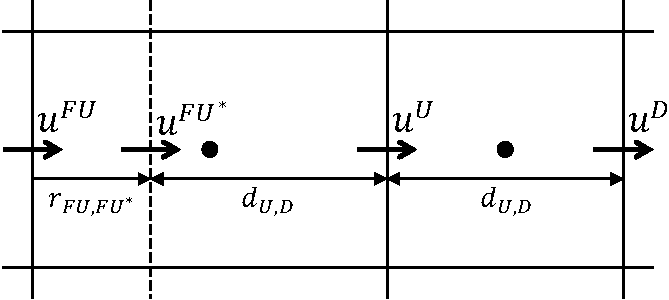
\includegraphics[width=0.75\textwidth]{non_uniform_cells_black.pdf}
	\caption[Non-uniform staggered grid]{Non-uniform staggered grid. The 
	distance between $u^{FU^*}$ and $u^U$ is the same that there is between 
	$u^U$ and $u^D$.}
	\label{fig:nonunifli}
\end{figure}

The idea is that if the grid is not uniform, the distances between $u^D$ and 
$u^U$ and between $u^U$ and $u^{FU}$ might be different, as it is represented 
in Figure~\ref{fig:nonunifli}. In this situation the formula 
\eqref{eq:tvdformula} can not be used directly, because the degree of freedom 
$u^{FU}$ is not at the position 
$u^{FU^*}$, where it would be if the grid was uniform, with cell sizes equal to 
the distance between $u^U$ and $u^D$, i.e. at the position upstream with 
respect to $u^U$, at a distance equal to the one between $u^U$ and $u^D$, see 
Figure~\ref{fig:nonunifli}. We want to use the ratio:
\begin{equation*}
r = \frac{u^U - u^{FU^*}}{u^D - u^U},
\end{equation*}
thus we need to build an approximation for $u^{FU^*}$.

\textcite{nonunif:darmou} proposed the following scheme that 
approximates the difference $u^D - u^{FU^*}$:
\begin{equation}
r = \frac{u^U - u^{FU^*}}{u^D - u^U} = \frac{(u^D - u^{FU^*})-(u^D - u^U)}{u^D 
- u^U} = \frac{u^D - u^{FU^*}}{u^D - u^U} - 1,
\end{equation}
\begin{equation}
u^D - u^{FU^*} \approx \frac{du^U}{dx} r_{ \scriptscriptstyle FU^*, D} = 2 
\frac{du^U}{dx} r_{\scriptscriptstyle U, D},
\end{equation}
where $r_{ \scriptscriptstyle A, B} $ denotes the vector from the point $A$ to 
$B$. \textcite{nonunif:li} showed that this method behaves well with parabolic 
solutions, but not so well with exponential solutions. So they proposed an 
improved approximation which introduces more upwind information:
\begin{equation}
r = \frac{u^U - u^{FU^*}}{u^D - u^U}, \quad u^{FU^*} \approx u^{FU} + 
\frac{d u^{FU}}{dx} r_{\scriptscriptstyle FU, FU^*}.
\end{equation}

\textcite{nonunif:hou} introduced a different and more rigorous approach. The 
idea in order to improve those described above was derived to consider not only 
the distances between the degrees of freedom, but also the sizes of the cells 
around them. Let us consider for example a non-uniform staggered grid as in 
Figure~\ref{fig:hou}.
\begin{figure*}[h]
	\centering
	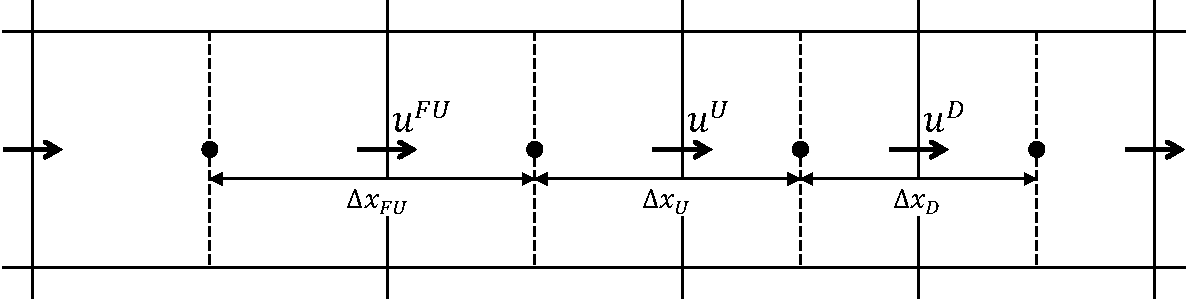
\includegraphics[width=\textwidth]{cells_with_sizes.pdf}
	\caption[Non-uniform staggered grid with cell sizes]{Non-uniform staggered 
	grid with cell sizes.}
	\label{fig:hou}
\end{figure*}
\\We generalize \eqref{eq:tvdformula} in the following way:
\begin{equation}
u^* = u^U + \frac{1}{\RUD} \psi(r) (u^D - u^U),
\end{equation}
\begin{equation}
\RUD = \frac{\Delta \xU + \Delta \xD}{\Delta \xU}, \quad r = \frac{u^U - 
u^{FU}}{x^U - x^{FU}} \cdot \frac{x^D - x^U}{u^D - u^U}.
\end{equation}
$\RUD$ takes into account the sizes of the upstream and downstream 
staggered cells, while $r$ is modified into ratio between an approximation of 
the gradients. Notice that if the grid is uniform $\RUD = 2$, as in the uniform 
formula \eqref{eq:tvdformula}.

Repeating the procedure described in the Subsection~\ref{subsec:tvd}, the TVD 
condition \eqref{eq:tvdcondition} and the second order accuracy are imposed, 
obtaining the following modified bounds for the flux limiter function $\psi$:
\begin{align}
\notag \psi(r) = 0 \quad &\text{if} \quad r < 0\\
r \leq \psi(r) \leq \min \bigg \{\frac{\RFUU}{\RFUU - 1}, 1 \bigg \} \quad 
&\text{if} \quad 0 \leq r \leq 1\\
\notag 1 \leq \psi(r) \leq \min \{r,\RUD \} \quad &\text{if} \quad r > 2
\end{align}
In Figure~\ref{fig:tvdregionhou} we can see the modified TVD region; with 
respect to Figure~\ref{fig:tvdregion}, the upper bounds are changed.
\begin{figure}[t]
	\centering
	% This file was created by matlab2tikz.
%
\begin{tikzpicture}

\begin{axis}[%
width=1.25\widthsette,
height=0.75\widthsette,
at={(0\widthsette,0\widthsette)},
scale only axis,
xmin=0,
xmax=4,
xlabel style={font=\color{white!15!black}},
xlabel={$r$},
ymin=0,
ymax=2.5,
ylabel style={font=\color{white!15!black}, rotate=-90},
ylabel={$\psi$},
axis background/.style={fill=white},
xmajorgrids,
ymajorgrids
]

\addplot[area legend, line width=1.0pt, draw=black, fill=white!80!black, fill opacity=0.5, forget plot]
table[row sep=crcr] {%
x	y\\
0	0\\
1	1\\
0.444444444444444	1\\
}--cycle;

\addplot[area legend, line width=1.0pt, draw=black, fill=white!80!black, fill opacity=0.5, forget plot]
table[row sep=crcr] {%
x	y\\
1	1\\
5.5	1\\
5.5	1.8\\
1.8	1.8\\
}--cycle;
\addplot [color=black, dashed, line width=1.0pt, forget plot]
  table[row sep=crcr]{%
0	1.8\\
1.8	1.8\\
};
\addplot [color=black, dashed, line width=1.0pt, forget plot]
  table[row sep=crcr]{%
0.444444444444444	1\\
1.11111111111111	2.5\\
};
\end{axis}

\begin{axis}[%
width=1.290\widthsette,
height=1.01\widthsette,
at={(-0.16\widthsette,-0.135\widthsette)},
scale only axis,
xmin=0,
xmax=1,
ymin=0,
ymax=1,
axis line style={draw=none},
ticks=none,
axis x line*=bottom,
axis y line*=left,
legend style={legend cell align=left, align=left, draw=white!15!black}
]
\node[below right, align=left, draw=none,]
at (rel axis cs:0.035,0.7) {\small$\RUD$};
\node[below right, align=left, draw=none]
at (rel axis cs:0.35,1) {\small $\dfrac{\RFUU}{\RFUU-1}r$};
\end{axis}
\end{tikzpicture}%
	\caption[Modified TVD region]{In grey the modified TVD region for 
	non-uniform grids in which the flux limiter functions must fit 
	\cite{nonunif:hou}.}
	\label{fig:tvdregionhou}
\end{figure} 
At last the flux limiter functions \eqref{eq:vl}--\eqref{eq:mclim} have to be 
generalized in order to fit into these new bounds.

\section{Cell-centred concept}
In the porous-medium region $\Omega_\text{pm}$ we have to solve only a steady 
scalar equation, with the 
pressure as a primary variable, indeed, due to the incompressibility of the 
fluid, the time derivative is not present:
\begin{align}
\label{eq:cellcentred}	\nabla \cdot \mathbf{v} = 0&\\
\label{eq:forch2}	\mathbf{v} + C_F \sqrt{\mathbf{K}} \frac{\varrho}{\mu} 
	|\mathbf{v}|\mathbf{v} + \frac{1}{\mu} \mathbf{K}(\nabla p - \varrho 
	\mathbf{g} ) = \mathbf{0}&
\end{align}
We employ a cell-centred finite volumes method, so the degrees of freedom of 
the pressure are located at the centre of each cell, as we can see in 
Figure~\ref{fig:cellcentred}, and the cells of the grid correspond to the 
control volumes.
\begin{figure}
	\centering
	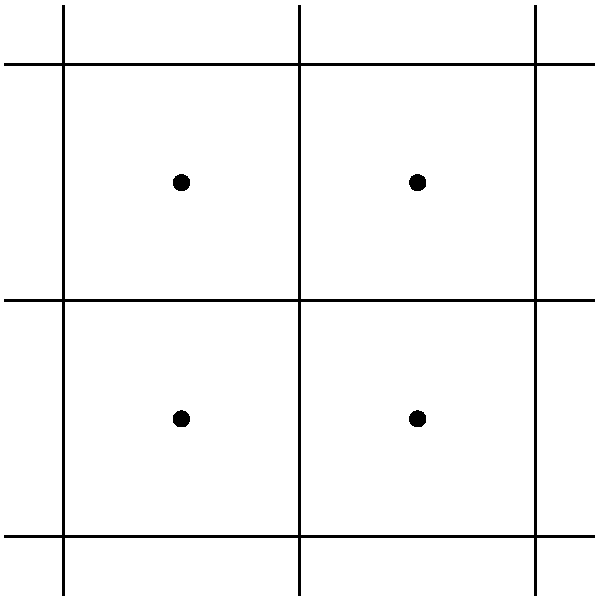
\includegraphics[width=0.4\textwidth]{cellcentred.pdf}
	\caption[Cell-centred grid]{Location of the degrees of freedom within a 
	cell-centred approach.}
	\label{fig:cellcentred}
\end{figure}

Let us integrate the equation \eqref{eq:cellcentred} over a control volume 
$V_L$ (see Figure~\ref{fig:cctpfa}) and apply the Gauss's divergence theorem:
\begin{equation}
\int_{V_L} \nabla \cdot \mathbf{v} \; dV = \int_{\partial V_L} \mathbf{v} \cdot 
\mathbf{n} \; dA.
\end{equation}
The Forchheimer's law \eqref{eq:forch2} is non-linear, so we use the Newton's 
method in order to compute the velocity, i.e. the flux over the boundary 
$\partial 
V_L$:
\begin{align}
	\mathbf{J}_f(\mathbf{v}^k) \delta \mathbf{v}^{k+1} =& 
	-\mathbf{f}(\mathbf{v}^k), \quad \text{$\forall k\geq 0$ until 
	convergence}\\
	\mathbf{v}^{k+1} =& \mathbf{v}^k + \delta \mathbf{v}^{k+1}
\end{align}
where
\begin{equation} \label{eq:resforch}
	\mathbf{f}(\mathbf{v}) = \mathbf{v} + C_F \sqrt{\mathbf{K}} 
	\frac{\varrho}{\mu} 
	|\mathbf{v}|\mathbf{v} + \frac{1}{\mu} \mathbf{K}(\nabla p - \varrho 
	\mathbf{g} )
\end{equation}
and $\mathbf{J}_f(\mathbf{v})$ is its Jacobian matrix:
\begin{equation} \label{eq:jacforch}
\mathbf{J}_f(\mathbf{v}) = \mathbb{1} + 
C_F\sqrt{\mathbf{K}}\frac{\varrho}{\mu}\big(|\mathbf{v}|\mathbb{1} + 
\frac{1}{|\mathbf{v}|}{\mathbf{v}\mathbf{v}^\mathrm{T}}\big).
\end{equation}
We use as initial guess $\mathbf{v}^0$ the velocity computed with the Darcy's 
law \eqref{eq:darcy}.

The evaluation of \eqref{eq:resforch} and \eqref{eq:jacforch} over $\partial 
V_L$ is performed with a Two Point Flux Approximation (TPFA) method, which 
consists in exploiting the values of the two cells sharing the face; it is a 
simple but robust method, commonly used in commercial software.
\begin{figure}
	\centering
	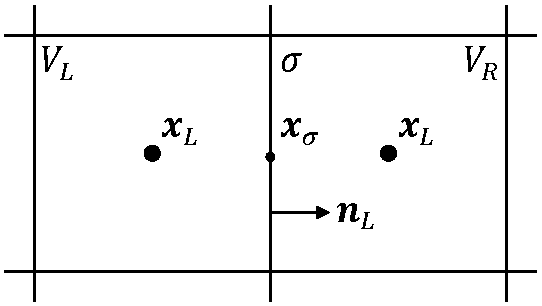
\includegraphics[width=0.6\textwidth]{cctpfa3.pdf}
	\caption[Two cells $V_L$ and $V_R$ sharing the face $\sigma$]{Two cells 
	$V_L$ and $V_R$ sharing the face $\sigma$.}
	\label{fig:cctpfa}
\end{figure}
Let us consider for instance the face $\sigma = \partial V_L \cup \partial 
V_R$, according to Figure~\ref{fig:cctpfa}, and let the permeability tensor be 
diagonal so that it act as a scalar. We approximate the derivative of the 
pressure $\partial p /\partial 
x$ with a centred finite difference:
\begin{equation}
\frac{\partial p}{\partial x} \approx \frac{p_R-p_L}{x_R -x_L}.
\end{equation}
We approximate the permeability $\mathbf{K}$ with its value at 
$\mathbf{x}_\sigma$, while 
for the viscosity $\mu$ (and eventually the density $\varrho$) we employ the 
upwind value.

In case of discontinuous permeabilities at the face $\sigma$, an harmonic 
average weighted on the distances between the cell centres and the face is 
performed:
\begin{equation}
\frac{|x_R - x_L|}{\mathrm{K}} \approx 
\frac{|x_\sigma - x_L|}{\mathrm{K}_L}+\frac{|x_R - x_\sigma|}{\mathrm{K}_R}.
\end{equation}

These formulas for the TPFA approximation are the simplified version for a 
Cartesian grid, while in the general case of an unstructured grid the method is 
derived exploiting a decomposition of the vector
\begin{equation}
\mathbf{d}_{L,\sigma}=\mathbf{x}_\sigma - \mathbf{x}_L,
\end{equation}
based the co-normal vector $\mathbf{Kn}_L$. Moreover it 
can be shown that this approximation is consistent only if the grid is 
K-orthogonal, i.e. if $\mathbf{Kn}_L$ is parallel to $\mathbf{d}_{L, \sigma}$ 
(see \cite{tesi:wolff}).
%\section{Coupling conditions}
% Disegno di cosa succede all'interfaccia
% Not sure about this section...
\section{Time discretization} \label{subsec:time}
The RANS equations have to be discretized also in time. Let us consider a 
generic unknown $\phi$ that could be a component of the velocity, the turbulent 
kinetic energy $k$ or its specific dissipation rate $\omega$. After the spatial 
discretization we obtain equations of the following kind:
\begin{equation} \label{eq:timegen}
	\frac{\partial \phi}{\partial t} = f(\phi, t),
\end{equation}
where the function $f$ at the right-hand side contains all the terms except the 
the time derivative. We introduce a discretization of the time 
interval $[0, T]$ into $N_t$ uniform time-steps, such that $\Delta t = T/Nt$ is 
the time-step size and $t^n=n\Delta t, \; n=0,\dots,N_t$. Let $\phi^n$ be the 
numerical solution at $t^n$. In order to 
discretize in time the equation \eqref{eq:timegen}, we have employed two 
implicit schemes.

\subsubsection{Backward Euler method}
The Backward Euler (BE) method (or implicit Euler method) consists in 
approximating the time derivative with a backward finite difference:
\begin{equation}
	\frac{\partial \phi}{\partial t} \approx \frac{	\phi^{n+1}-\phi^n}{\Delta 
	t} = f(\phi^{n+1}, t^{n+1}).
\end{equation}
In terms of global truncation error, it converges with order 1 and it is 
unconditionally stable, so no particular attention must be paid to the choice 
of $\Delta t$ in order to guarantee the stability. Of course an initial 
condition $\phi^0$ must be provided.
%
\subsubsection{BDF2 method}
The Backward Differencing Formula 2 (BDF2) method consists in approximating the 
time derivative with a backward finite difference of second order:
\begin{equation}
	\frac{\partial \phi}{\partial t} \approx 
	\frac{3\phi^{n+1}-4\phi^n+\phi^{n-1}}{2\Delta t} = f(\phi^{n+1}, t^{n+1}).
\end{equation}
In terms of global truncation error, it converges with order 2 and it is 
unconditionally stable too. It is a two-step method because it requires two 
initial conditions; this is a problem at the very first time step because we 
would need to know $\phi^{-1}$. This issue is usually solved performing one 
iteration with a one-step method, the BE usually, and then starting with the 
BDF2 from the second iteration. This trick does not affect the overall 
convergence order because a single step of a first order one-step method 
introduces a local truncation error second order.
	
The method can be generalized to case of non constant time-steps. Let us define 
$\Delta t^n=t^n-t^{n-1}, \; n=1,\dots,N_t$, then the scheme becomes:
\begin{multline}
	\frac{\partial \phi}{\partial t} \approx \frac{\phi^{n+1}\Delta 
	t^n(2\Delta t^{n+1}+\Delta t^n)-\phi^n(\Delta t^{n+1}+\Delta 
	t^n)^2+\phi^{n-1}(\Delta t^{n+1})^2}{\Delta 
	t^{n+1}\Delta t^n(\Delta t^n+\Delta t^{n+1})} =\\
= f(\phi^{n+1}, t^{n+1})
\end{multline}
See \cite{main:matenum} for more detailed information about time discretization 
methods.
\section{Summary}
Fully implicit coupling, monolithic approach, UMFPACK, cenni alle coupling 
conditions and boundary conditions, primary variables. Jacobian numerically The 
time-step size depends of the 
convergence of the Newton's method at the previous time iteration.
\chapter{Numerical results} \label{chap:results}
In this chapter we present some numerical results. The convergence of higher 
order methods applied to the Navier-Stokes equations is tested, first in space, 
then in time. Then another spatial comparison test between the upwind method 
and the TVD methods is performed using a channel flow. After that the results 
from the backward facing step test using the RANS equations are shown and 
compared to those from the CFL3D code \cite{web:nasa}. Next, a turbulent 
channel flow with two small cavities is studied and at last a coupled free-flow 
and porous-medium flow problem is analysed, varying the permeability of the 
porous-medium.\\
In all the tests the gravity has been neglected.
%
\section{Navier-Stokes tests}
\subsection{Space convergence} \label{subsec:conv}
We want to test the spatial convergence order of the $L^2$-error of the 
solution of the Navier-Stokes equations, comparing the results obtained with 
the upwind method \eqref{eq:upwind} and the TVD methods described in 
Subsection~\ref{subsec:tvd}.\\
We consider a steady version of the 
equations~\eqref{eq:nsmass}--\eqref{eq:nsmom}:
\begin{align}
	\label{eq:nssteadymass} \nabla \cdot \mathbf{v} -h = 0&\\
	\label{eq:nssteadymom} \nabla \cdot (\mathbf{v} \mathbf{v}^\mathrm{T}) - 
	\nabla \cdot (\nu \nabla \mathbf{v}) + \frac{1}{\varrho}\nabla p  
	-\mathbf{f} = \mathbf{0}&
\end{align}
We neglect the gravity, but we take into account two possible source terms 
$h$ and $\mathbf{f}$. Moreover, for the sake of simplicity, we consider here 
all the quantities appearing in the equations to be non-dimensional.
%
\subsubsection{Sin-Cos test}
Let us solve the equations~\eqref{eq:nssteadymass}--\eqref{eq:nssteadymom} over 
a two-dimensional unit domain $\Omega=(0,1)^2$, with the following source terms:
\begin{align}
	h &= 0,\\
	\mathbf{f} &= [-2\nu \cos(x) \sin(y), \; 2\nu \cos(y) \sin(x)]^\mathrm{T},
\end{align}
so that, choosing $\varrho=1$, the analytical solution, depicted in 
Figure~\ref{fig:sincosexact}, is given by
\begin{align}
\label{eq:uexsin}	u_\text{ex}(x,y) &= -\cos(x)\sin(y)\\
	v_\text{ex}(x,y) &= \sin(x)\cos(y)\\
\label{eq:pexsin}	p_\text{ex}(x,y) &= -\frac{\cos(2x)+\sin(2y)}{4}
\end{align}
Dirichlet boundary conditions for the velocity are applied on the whole 
boundary $\partial \Omega$ using the exact solution. Because of this choice, 
the pressure appears in the problem only in the momentum equation 
\eqref{eq:nssteadymom}, under the sign of gradient. Thus in the numerical 
solution it would be defined up to a constant, so we fix its value at one point 
in the domain in order to match the exact solution \eqref{eq:pexsin}.
\begin{figure}
	\centering
	\subfloat{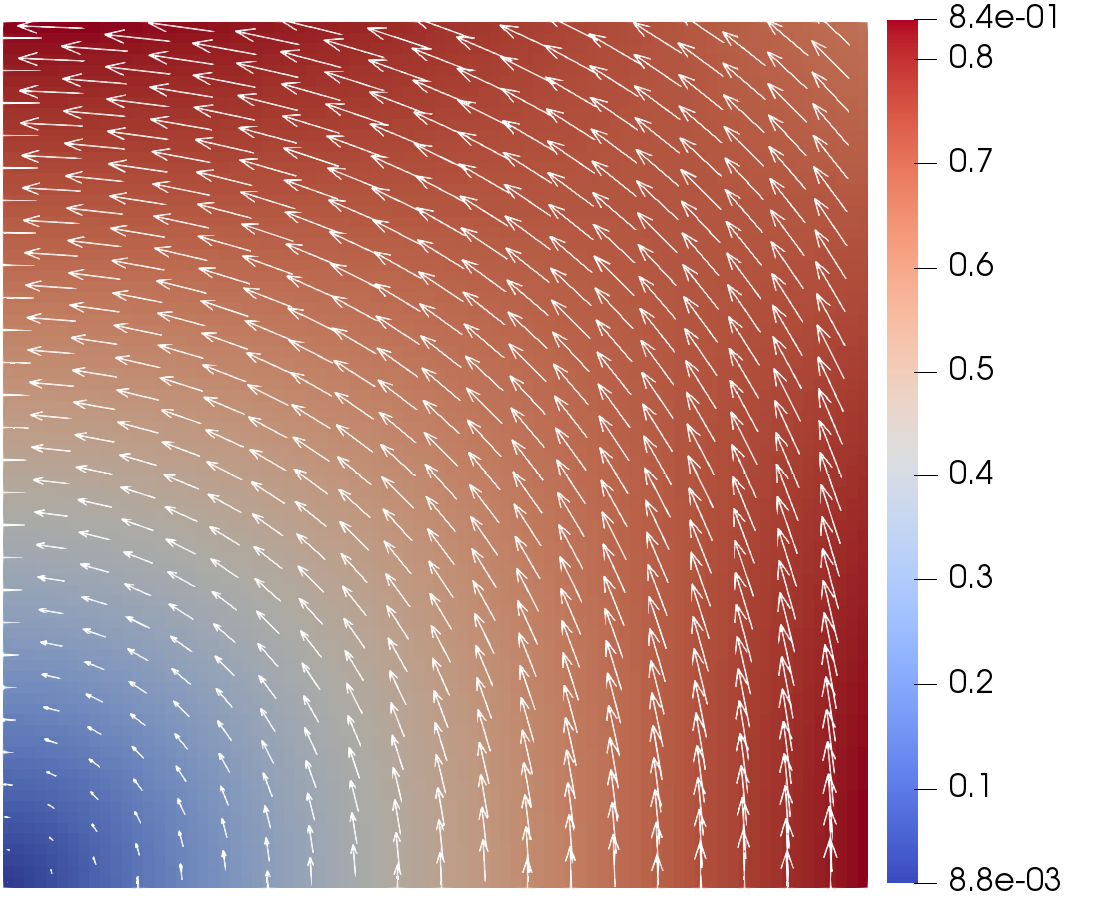
\includegraphics[width=0.5\textwidth]{sincos_exact_v_report.png}}
	\subfloat{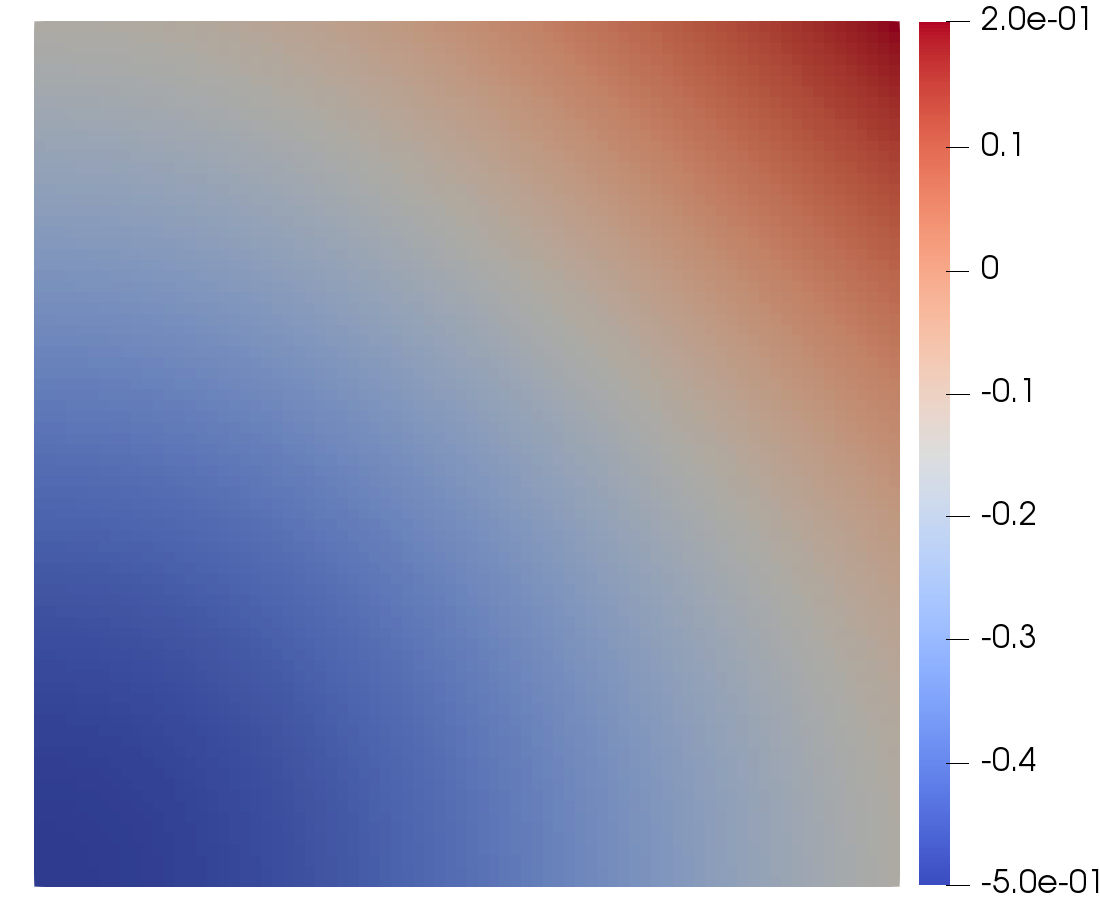
\includegraphics[width=0.5\textwidth]{sincos_exact_p_report.png}}
	\caption[Exact solution of the Sin-Cos test]{Exact solution of the Sin-Cos 
	test \eqref{eq:uexsin}--\eqref{eq:pexsin}. On the left the magnitude of the 
	velocity field, on the right the 
	pressure field.}
	\label{fig:sincosexact}
\end{figure}

The problem is solved over a sequence of five uniform grids, starting from 
$\num{4x4}$ cells and each time halving their size. Both the cases of $\nu=1$ 
and $\nu=\num{e-3}$ are considered, that correspond to $Re=1$ and $Re=\num{e3}$ 
respectively. In Figure~\ref{fig:sin_err} the errors computed are reported 
depending on the square root of the number of cells, while in 
Tables~\ref{tab:sin_lre}--\ref{tab:sin_hre} we can compare directly the 
convergence orders for the different differencing schemes.
\begin{figure}
	\centering
	\subfloat[Upwind, $Re = 1$]{
		% This file was created by matlab2tikz.
%
\definecolor{mycolor1}{rgb}{0.00000,0.44700,0.74100}%
\definecolor{mycolor2}{rgb}{0.85000,0.32500,0.09800}%
\definecolor{mycolor3}{rgb}{0.92900,0.69400,0.12500}%
%
\begin{tikzpicture}

\begin{axis}[%
width=0.951\figwidth,
height=0.75\figwidth,
at={(0\figwidth,0\figwidth)},
scale only axis,
xmode=log,
xmin=4,
xmax=100,
xminorticks=true,
ymode=log,
ymin=1e-05,
ymax=0.1,
yminorticks=true,
axis background/.style={fill=white},
legend style={at={(0.97,0.97)}, anchor=north east, legend cell align=left, align=left, draw=white!15!black}
]
\addplot [color=mycolor1, mark=x, mark options={solid, mycolor1}]
  table[row sep=crcr]{%
4	0.0377253281\\
8	0.016292839\\
16	0.00647505826\\
32	0.00277859939\\
64	0.00131783073\\
};
\addlegendentry{$p$}

\addplot [color=mycolor2, mark=x, mark options={solid, mycolor2}]
  table[row sep=crcr]{%
4	0.00100309389\\
8	0.000409725552\\
16	0.000134946447\\
32	5.06672786e-05\\
64	2.29407924e-05\\
};
\addlegendentry{$u$}

\addplot [color=mycolor3, mark=x, mark options={solid, mycolor3}]
  table[row sep=crcr]{%
4	0.000631316968\\
8	0.000278812074\\
16	0.00010907144\\
32	4.76177485e-05\\
64	2.28652417e-05\\
};
\addlegendentry{$v$}

\addplot [color=white!70!black, forget plot]
  table[row sep=crcr]{%
4	0.00025\\
100	1e-05\\
};
\addplot [color=white!70!black, forget plot]
  table[row sep=crcr]
	\subfloat[Upwind, $Re = \num{e3}$]{
		% This file was created by matlab2tikz.
%
\definecolor{mycolor1}{rgb}{0.00000,0.44700,0.74100}%
\definecolor{mycolor2}{rgb}{0.85000,0.32500,0.09800}%
\definecolor{mycolor3}{rgb}{0.92900,0.69400,0.12500}%
%
\begin{tikzpicture}

\begin{axis}[%
width=0.951\figwidth,
height=0.75\figwidth,
at={(0\figwidth,0\figwidth)},
scale only axis,
xmode=log,
xmin=4,
xmax=100,
xminorticks=true,
ymode=log,
ymin=0.00266295649,
ymax=0.1,
yminorticks=true,
axis background/.style={fill=white},
legend style={at={(0.97,0.97)}, anchor=north east, legend cell align=left, align=left}
]
\addplot [color=mycolor1, mark=x, mark options={solid, mycolor1}]
  table[row sep=crcr]{%
4	0.0596083589\\
8	0.0364982308\\
16	0.0196434526\\
32	0.00962257784\\
64	0.00434161729\\
};
\addlegendentry{$p$}

\addplot [color=mycolor2, mark=x, mark options={solid, mycolor2}]
  table[row sep=crcr]{%
4	0.0339372138\\
8	0.0206751686\\
16	0.011131246\\
32	0.00559430586\\
64	0.00266295649\\
};
\addlegendentry{$u$}

\addplot [color=mycolor3, mark=x, mark options={solid, mycolor3}]
  table[row sep=crcr]{%
4	0.0347600515\\
8	0.0213374017\\
16	0.0114856296\\
32	0.00577467407\\
64	0.00275450966\\
};
\addlegendentry{$v$}

\addplot [color=white!70!black, forget plot]
  table[row sep=crcr]{%
4	0.06657391225\\
100	0.00266295649\\
};
\addplot [color=white!70!black, forget plot]
  table[row sep=crcr]\\
	\subfloat[Min-Mod, $Re = 1$]{
		% This file was created by matlab2tikz.
%
\definecolor{mycolor1}{rgb}{0.00000,0.44700,0.74100}%
\definecolor{mycolor2}{rgb}{0.85000,0.32500,0.09800}%
\definecolor{mycolor3}{rgb}{0.92900,0.69400,0.12500}%
%
\begin{tikzpicture}

\begin{axis}[%
width=0.951\figwidth,
height=0.75\figwidth,
at={(0\figwidth,0\figwidth)},
scale only axis,
xmode=log,
xmin=4,
xmax=100,
xminorticks=true,
ymode=log,
ymin=1e-05,
ymax=0.1,
yminorticks=true,
axis background/.style={fill=white},
legend style={at={(0.97,0.97)}, anchor=north east, legend cell align=left, align=left}
]
\addplot [color=mycolor1, mark=x, mark options={solid, mycolor1}]
  table[row sep=crcr]{%
4	0.0201961443\\
8	0.00658170291\\
16	0.00181646151\\
32	0.000558641084\\
64	0.000188245776\\
};
\addlegendentry{$p$}

\addplot [color=mycolor2, mark=x, mark options={solid, mycolor2}]
  table[row sep=crcr]{%
4	0.00148598782\\
8	0.00053497283\\
16	0.000150385476\\
32	3.95894587e-05\\
64	1.01636468e-05\\
};
\addlegendentry{$u$}

\addplot [color=mycolor3, mark=x, mark options={solid, mycolor3}]
  table[row sep=crcr]{%
4	0.00119526142\\
8	0.00045470553\\
16	0.000138075359\\
32	3.80865907e-05\\
64	1.00057526e-05\\
};
\addlegendentry{$v$}

\addplot [color=white!70!black, forget plot]
  table[row sep=crcr]{%
4	0.00025\\
100	1e-05\\
};
\addplot [color=white!70!black, forget plot]
  table[row sep=crcr]
	\subfloat[Min-Mod, $Re = \num{e3}$]{
		% This file was created by matlab2tikz.
%
\definecolor{mycolor1}{rgb}{0.00000,0.44700,0.74100}%
\definecolor{mycolor2}{rgb}{0.85000,0.32500,0.09800}%
\definecolor{mycolor3}{rgb}{0.92900,0.69400,0.12500}%
%
\begin{tikzpicture}

\begin{axis}[%
width=0.951\figwidth,
height=0.75\figwidth,
at={(0\figwidth,0\figwidth)},
scale only axis,
xmode=log,
xmin=4,
xmax=100,
xminorticks=true,
ymode=log,
ymin=0.0001,
ymax=0.0206930353,
yminorticks=true,
axis background/.style={fill=white},
legend style={at={(0.97,0.97)}, anchor=north east, legend cell align=left, align=left}
]
\addplot [color=mycolor1, mark=x, mark options={solid, mycolor1}]
  table[row sep=crcr]{%
4	0.0206930353\\
8	0.0102262223\\
16	0.00364544433\\
32	0.000812298263\\
64	0.000257143964\\
};
\addlegendentry{$p$}

\addplot [color=mycolor2, mark=x, mark options={solid, mycolor2}]
  table[row sep=crcr]{%
4	0.0130268788\\
8	0.00605072242\\
16	0.00243635311\\
32	0.000918041806\\
64	0.000338134479\\
};
\addlegendentry{$u$}

\addplot [color=mycolor3, mark=x, mark options={solid, mycolor3}]
  table[row sep=crcr]{%
4	0.0129926934\\
8	0.00750558766\\
16	0.0037160882\\
32	0.00148526754\\
64	0.000512917943\\
};
\addlegendentry{$v$}

\addplot [color=white!70!black, forget plot]
  table[row sep=crcr]{%
4	0.0025\\
100	0.0001\\
};
\addplot [color=white!70!black, forget plot]
  table[row sep=crcr]\\
	\subfloat[Van Leer, $Re = 1$]{
		% This file was created by matlab2tikz.
%
\definecolor{mycolor1}{rgb}{0.00000,0.44700,0.74100}%
\definecolor{mycolor2}{rgb}{0.85000,0.32500,0.09800}%
\definecolor{mycolor3}{rgb}{0.92900,0.69400,0.12500}%
%
\begin{tikzpicture}

\begin{axis}[%
width=0.951\figwidth,
height=0.75\figwidth,
at={(0\figwidth,0\figwidth)},
scale only axis,
xmode=log,
xmin=4,
xmax=100,
xminorticks=true,
ymode=log,
ymin=8.63199669e-06,
ymax=0.1,
yminorticks=true,
axis background/.style={fill=white},
legend style={at={(0.03,0.03)}, anchor=south west, legend cell align=left, align=left, draw=white!15!black}
]
\addplot [color=mycolor1, mark=x, mark options={solid, mycolor1}]
  table[row sep=crcr]{%
4	0.017335487\\
8	0.0062618753\\
16	0.00193371119\\
32	0.000605597659\\
64	0.000196206927\\
};
\addlegendentry{$p$}

\addplot [color=mycolor2, mark=x, mark options={solid, mycolor2}]
  table[row sep=crcr]{%
4	0.00136409678\\
8	0.000476275877\\
16	0.000131606902\\
32	3.41242821e-05\\
64	8.66824542e-06\\
};
\addlegendentry{$u$}

\addplot [color=mycolor3, mark=x, mark options={solid, mycolor3}]
  table[row sep=crcr]{%
4	0.00114596769\\
8	0.000417513208\\
16	0.000122988533\\
32	3.32359157e-05\\
64	8.63199669e-06\\
};
\addlegendentry{$v$}

\addplot [color=white!70!black, forget plot]
  table[row sep=crcr]{%
4	0.00021579991725\\
100	8.63199669e-06\\
};
\addplot [color=white!70!black, forget plot]
  table[row sep=crcr]
	\subfloat[Van Leer, $Re = \num{e3}$]{
		% This file was created by matlab2tikz.
%
\definecolor{mycolor1}{rgb}{0.00000,0.44700,0.74100}%
\definecolor{mycolor2}{rgb}{0.85000,0.32500,0.09800}%
\definecolor{mycolor3}{rgb}{0.92900,0.69400,0.12500}%
%
\begin{tikzpicture}

\begin{axis}[%
width=0.951\figwidth,
height=0.75\figwidth,
at={(0\figwidth,0\figwidth)},
scale only axis,
xmode=log,
xmin=4,
xmax=100,
xminorticks=true,
ymode=log,
ymin=0.0001,
ymax=0.01454297,
yminorticks=true,
axis background/.style={fill=white},
legend style={at={(0.97,0.97)}, anchor=north east, legend cell align=left, align=left}
]
\addplot [color=white!70!black, forget plot, line width=0.75pt]
  table[row sep=crcr]{%
4	0.0025\\
100	0.0001\\
};
\addplot [color=white!70!black, forget plot, line width=0.75pt]
  table[row sep=crcr]{%
4	0.0625\\
100	0.0001\\
};
\addplot [color=mycolor1, mark=x, mark options={solid, mycolor1}, line width=0.75pt]
  table[row sep=crcr]{%
4	0.01454297\\
8	0.00653869074\\
16	0.00224775854\\
32	0.0005196908\\
64	0.000249600967\\
};
\addlegendentry{$p$}

\addplot [color=mycolor2, mark=x, mark options={solid, mycolor2}, line width=0.75pt]
  table[row sep=crcr]{%
4	0.0107200353\\
8	0.00466675248\\
16	0.00177426299\\
32	0.000645881865\\
64	0.000238530337\\
};
\addlegendentry{$u$}

\addplot [color=mycolor3, mark=x, mark options={solid, mycolor3}, line width=0.75pt]
  table[row sep=crcr]
	\caption[$L^2$-errors for the Sin-Cos test]{$L^2$-errors for the Sin-Cos 
	test depending on the square root of the number of cells in the grid. 
	The grey lines are the reference lines for the first-order and second-order 
	convergence.}
	\label{fig:sin_err}
\end{figure}

\begin{table}
	\centering
	\[
	\begin{array}{c|ccc}
	\toprule
	& \text{Upwind} & \text{Min-Mod} & \text{Van Leer} \\ 
	\midrule
	p & 1.008 & 1.569 & 1.626\\
	v_x & 1.143 & 1.962 & 1.977\\
	v_y & 1.058 & 1.928 & 1.945\\
	\bottomrule
	\end{array}
	\]
	\caption[Convergence orders with $Re = 1$ for the Sin-Cos 
	test]{Convergence orders with $Re = 1$ for the Sin-Cos test. They are 
	computed considering the last two refinements of the grid.}
	\label{tab:sin_lre}
	\[
	\begin{array}{c|ccc}
	\toprule
	& \text{Upwind} & \text{Min-Mod} & \text{Van Leer} \\ 
	\midrule
	p & 1.148 & 1.659 & 1.058\\
	v_x & 1.071 & 1.441 & 1.437\\
	v_y & 1.068 & 1.533 & 1.560\\
	\bottomrule
	\end{array}
	\]
	\caption[Convergence orders with $Re = \num{e3}$ for the Sin-Cos 
	test]{Convergence orders with $Re = \num{e3}$ for the Sin-Cos test. 
	They are computed considering the last two refinements of the grid.}
	\label{tab:sin_hre}
\end{table}

We observe, as expected, a better behaviour of the TVD methods with respect to 
the upwind method. In Table~\ref{tab:sin_lre} we can see that at $Re=1$ the 
formers show a full second order convergence for the velocity, while for the 
rate is a bit lower; the latter instead shows a first for all the variables. At 
$Re=\num{e3}$ a slight decrease of the rates of the TVD methods occurs also for 
the velocities, but they remain higher then the ones of the upwind method. In 
Table~\ref{tab:sin_hre} we observe a convergence order of 1 for the pressure 
using the Van Leer flux limiter, but looking at Figure~\ref{fig:sin_err} we can 
see that the global trend indicates a convergence of higher order. Moreover it 
can be observed how, thanks to the faster convergence, on the same grid the 
absolute values of the errors reach smaller values using the TVD methods. 
Between the Min-Mod and Van Leer flux limiter it is hard to say which performs 
better, the results are very similar.

Analogous tests with other analytical solutions are reported in the 
Appendix~\ref{app:conv}. They show always a better convergence of the TVD 
methods with respect to the upwind method, but in some cases the convergence 
order of pressure and velocity behave differently.
%
\subsection{Time convergence}
We test the time convergence of the $L^\infty(0,T;L^2(\Omega))$ norm of the 
error of the solution of the Navier-Stokes equations, comparing the results 
obtained with the BE method \eqref{eq:be} and the BDF2 method \eqref{eq:bdf2}.\\
We consider the unsteady version of the 
equations~\eqref{eq:nssteadymass}--\eqref{eq:nssteadymom}:
\begin{align}
	\label{eq:nsunsteadymass} \nabla \cdot \mathbf{v} -h = 0&\\
	\label{eq:nsunsteadymom} \frac{\partial \mathbf{v}}{\partial t} +\nabla 
	\cdot (\mathbf{v} \mathbf{v}^\mathrm{T}) - 
	\nabla \cdot (\nu \nabla \mathbf{v}) + \frac{1}{\varrho}\nabla p  
	-\mathbf{f} = \mathbf{0}&
\end{align}
Again the gravity is neglected and two possible sources $h$ and $\mathbf{f}$ 
are taken into account, moreover all the quantities are considered to be 
non-dimensional.
%
\subsubsection{Unsteady Sin-Cos test}
Let us solve the equations~\eqref{eq:nsunsteadymass}--\eqref{eq:nsunsteadymom} 
over a two dimensional unit domain $\Omega=(0,1)^2$ and in the time interval 
$(0,T)$, with $T=1$. We use the following source terms:
\begin{align}
h &= 0,\\
\mathbf{f} &= 2\Big(\frac{\cos(2t)}{\varrho} + \nu \sin(2t)\Big)[- \cos(x) 
\sin(y), \; 
\cos(y) \sin(x)]^\mathrm{T},
\end{align}
so that, choosing $\varrho=1$, the analytical solution is given by
\begin{align}
\label{eq:uexunssin}	u_\text{ex}(x,y) &= -\cos(x)\sin(y)\sin(2t)\\
v_\text{ex}(x,y) &= \sin(x)\cos(y)\sin(2t)\\
\label{eq:pexunssin}	p_\text{ex}(x,y) &= 
-\frac{\cos(2x)+\sin(2y)}{4}\sin^2(2t),
\end{align}
so it is equal to \eqref{eq:uexsin}--\eqref{eq:pexsin}, used in the steady test 
for the space convergence, except for the modulation over time. We choose 
$\nu=0.1$, so that $Re=10$. Dirichlet boundary conditions for the velocity are 
applied on the whole boundary $\partial \Omega$ using the exact solution. 
Pressure is again fixed  at one point in order to match the exact solution 
\eqref{eq:pexunssin}.

The problem is solved seven times subdividing the time interval $(0,T)$ into 
uniform time-steps and each time time doubling their number, starting from a 
single time-step. Uniform grids of $\num{40x40}$ and $\num{80x80}$ cells are 
employed and as a differencing scheme the TVD method with the Van Leer flux 
limiter \eqref{eq:vl} is used. From Figure~\ref{fig:timeerr} we observe that, 
as expected, the BE method shows a first-order convergence, while the BDF2 
method is of second order. Moreover we notice that, with a grid of 
$\num{40x40}$ cells, in the last refinement the error with the BDF2 method does 
not decrease anymore. This happens because the spatial error becomes 
dominant, indeed refining the grid the convergence order is restored entirely 
for the pressure and almost for the velocity.
\begin{figure}
	\centering
	\subfloat{% This file was created by matlab2tikz.
%
\definecolor{mycolor1}{rgb}{0.00000,0.44700,0.74100}%
\definecolor{mycolor2}{rgb}{0.85000,0.32500,0.09800}%
\definecolor{mycolor3}{rgb}{0.92900,0.69400,0.12500}%
%
\begin{tikzpicture}

\begin{axis}[%
width=0.99\figwidth,
height=0.8\figwidth,
at={(0\figwidth,0\figwidth)},
scale only axis,
xmode=log,
xmin=1,
xmax=100,
xminorticks=true,
xlabel={$N_t$},
ymode=log,
ymin=0.0001,
ymax=1,
yminorticks=true,
%ylabel style={font=\scriptsize},
%ylabel={$L^\infty$-error},
axis background/.style={fill=white},
legend style={at={(0.03,0.03)}, anchor=south west, legend cell align=left, fill=none,
align=left, font=\scriptsize}
]
\addplot [color=mycolor1, mark=x, mark options={solid, mycolor1}]
  table[row sep=crcr]{%
1	2.91e-1\\
2	1.619e-1\\
4	8.07e-2\\
8	4.17e-2\\
16	2.1e-2\\
32	1.054e-2\\
64	5.31e-3\\
};
\addlegendentry{BE ($\num{40x40}$)}

\addplot [color=mycolor2, mark=x, mark options={solid, mycolor2}]
  table[row sep=crcr]{%
1	2.91e-1\\
2	1e-1\\
4	2.686e-2\\
8	6.81e-3\\
16	1.7e-3\\
32	4.23e-4\\
64	3.816e-4\\
};
\addlegendentry{BDF2 ($\num{40x40}$)}

\addplot [color=mycolor3, mark=x, mark options={solid, mycolor3}]
  table[row sep=crcr]{%
1	2.91e-1\\
2	1e-1\\
4	2.686e-2\\
8	6.814e-3\\
16	1.704e-3\\
32	4.258e-4\\
64	1.347e-4\\
};
\addlegendentry{BDF2 ($\num{80x80}$)}

\addplot [color=white!70!black, forget plot]
  table[row sep=crcr]{%
1	1\\
100	0.01\\
};
\addplot [color=white!70!black, forget plot]
  table[row sep=crcr]
	\subfloat{% This file was created by matlab2tikz.
%
\definecolor{mycolor1}{rgb}{0.00000,0.44700,0.74100}%
\definecolor{mycolor2}{rgb}{0.85000,0.32500,0.09800}%
\definecolor{mycolor3}{rgb}{0.92900,0.69400,0.12500}%
%
\begin{tikzpicture}

\begin{axis}[%
width=0.99\figwidth,
height=0.8\figwidth,
at={(0\figwidth,0\figwidth)},
scale only axis,
xmode=log,
xmin=1,
xmax=100,
xminorticks=true,
xlabel={$N_t$},
ymode=log,
ymin=1e-5,
ymax=1e-1,
yminorticks=true,
%ylabel style={font=\scriptsize},
%ylabel={$L^\infty$-error},
axis background/.style={fill=white},
legend style={at={(0.03,0.03)}, anchor=south west, legend cell align=left, fill=none,
align=left, font=\scriptsize}
]
\addplot [color=mycolor1, mark=x, mark options={solid, mycolor1}]
  table[row sep=crcr]{%
1	5.516e-2\\
2	3.043e-2\\
4	1.607e-2\\
8	8.216e-3\\
16	4.12e-3\\
32	2.03e-3\\
64	9.712e-4\\
};
\addlegendentry{BE ($\num{40x40}$)}

\addplot [color=mycolor2, mark=x, mark options={solid, mycolor2}]
  table[row sep=crcr]{%
1	5.516e-2\\
2	1.645e-2\\
4	4.8e-3\\
8	1.21e-3\\
16	2.85e-4\\
32	1.3e-4\\
64	1.278e-4\\
};
\addlegendentry{BDF2 ($\num{40x40}$)}

\addplot [color=mycolor3, mark=x, mark options={solid, mycolor3}]
  table[row sep=crcr]{%
1	5.42e-2\\
2	1.647e-2\\
4	4.83e-3\\
8	1.231e-3\\
16	3.024e-4\\
32	7.061e-5\\
64	3.6e-5\\
};
\addlegendentry{BDF2 ($\num{80x80}$)}

\addplot [color=white!70!black, forget plot]
  table[row sep=crcr]{%
1	0.1\\
100	0.001\\
};
\addplot [color=white!70!black, forget plot]
  table[row sep=crcr]
	\caption[$L^\infty(0,T;L^2(\Omega))$-errors for the unsteady Sin-Cos 
	test]{$L^\infty(0,T;L^2(\Omega))$-errors for the unsteady Sin-Cos test 
	depending on the number of time-steps. On the left the errors for the 
	pressure, on the right the error for the magnitude of the velocity. The 
	grey lines are the reference lines for the first-order and second-order 
	convergence.}
	\label{fig:timeerr}
\end{figure}
%
\subsection{Rough channel test}
We test the behaviour of the TVD methods compared to the upwind method, applied 
to the unsteady Navier-Stokes equations \eqref{eq:nsmass}--\eqref{eq:nsmom}, in 
a channel flow with a rough (i.e. non-flat) lower boundary. The roughness 
consists in small cavities evenly spaced cavities. Two different configurations 
are studied, one with shallow cavities (Figure~\ref{fig:roughdom}) and another 
with deeper cavities (Figure~\ref{fig:roughdomdeep}).

On the left boundary $\Gamma_\text{in}$ we set inflow boundary conditions 
\eqref{eq:inflow}, specifying an horizontal velocity
\begin{equation}
	\mathbf{v} = \mathbf{v}_\text{in} = [u_\text{in}, 0]^\mathrm{T}, \quad 
	u_\text{in} = \SI{1}{m/s}.
\end{equation}
On the lower and upper boundaries $\Gamma_w$ we set no-slip boundary conditions 
\eqref{eq:noslip}, while on the right boundary $\Gamma_\text{out}$ we set 
outflow boundary conditions \eqref{eq:outflow}, fixing the value of the pressure
\begin{equation}
	p = p_\text{ext} = \SI{1.1e5}{\pascal}.
\end{equation}
As initial conditions the velocity is set to zero everywhere, while the 
pressure is set to $p_\text{ext}$ everywhere. The density is 
$\varrho=\SI{1}{kg/m^3}$. The gravity contribution in \eqref{eq:nsmom} is 
neglected.
%
\subsubsection{Shallow cavities}
\begin{figure}
	\centering
	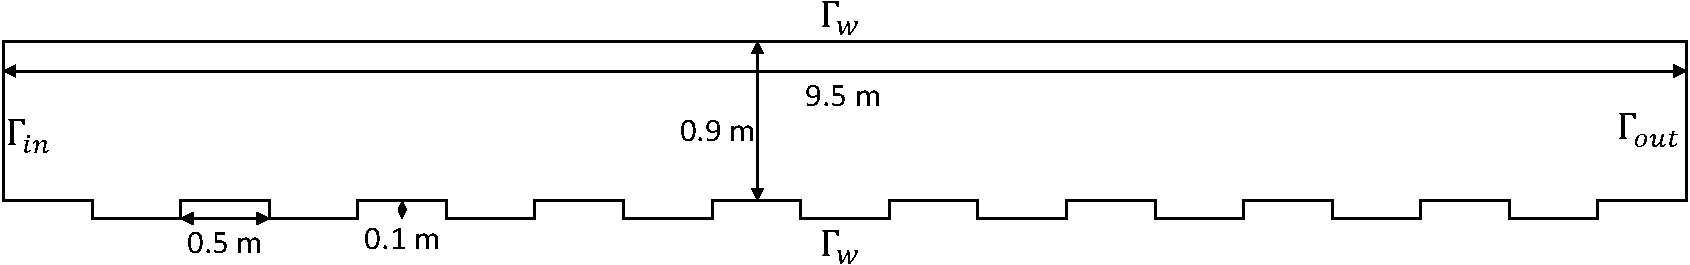
\includegraphics[width=\textwidth]{rough_domain2.pdf}
	\caption[Domain of the rough channel test with shallow cavities]{Domain of 
	the rough channel test with shallow cavities.}
	\label{fig:roughdom}
\end{figure}
\begin{figure}
	\centering
	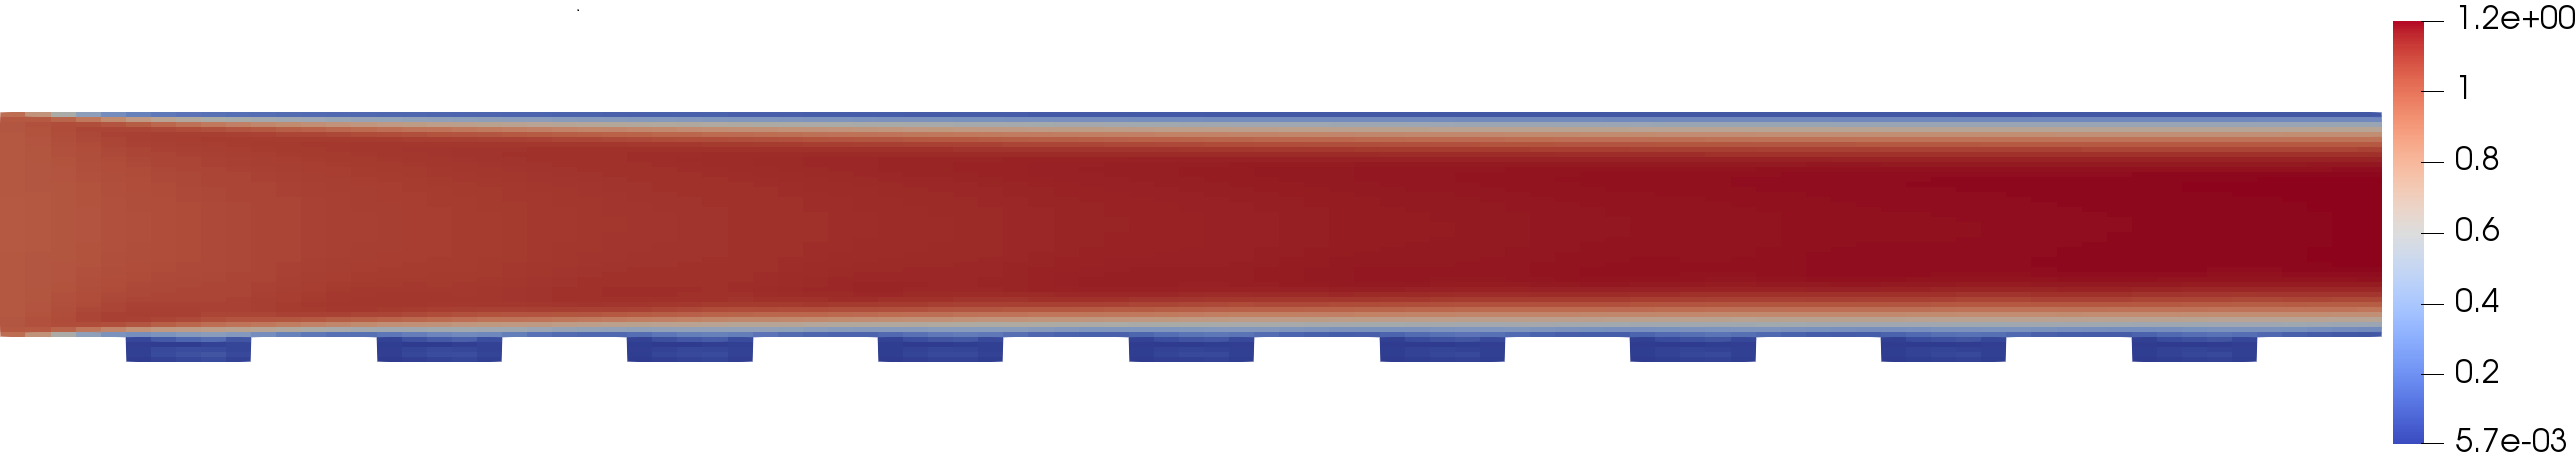
\includegraphics[width=\textwidth]{rough_channel_vl_report.png}
	\caption[Velocity magnitude in the rough channel test with shallow 
	cavities]{Velocity magnitude in the rough channel test with shallow 
	cavities at $t=\SI{10}{s}$. $Re=\num{2e3}$, Van Leer flux limiter.}
	\label{fig:roughchannelvl}
\end{figure}
\begin{table}
	\centering
	\[
	\begin{array}{ccc}
	\toprule
	\text{Upwind} & \text{Van Leer} & \text{Van Alabada} \\
	\midrule
	\num{1.708e-4} & \num{9.556e-6} & \num{1.119e-5} \\
	\midrule
	\text{Min-Mod} & \text{Superbee} & \text{MC Limiter} \\
	\midrule
	\num{1.537e-5} &  \SI{8.335e-6} & \num{8.659e-6}\\
	\bottomrule
	\end{array}
	\]
	\caption[$L^2$-errors for the velocity in the rough channel with shallow 
	cavities]{$L^2$-errors for the velocity along a section at $x=\SI{8.75}{m}$ 
	and $t=\SI{10}{s}$ in the rough channel with shallow cavities. $Re = 
	\num{2e3}$.}
	\label{tab:errshallow}
\end{table}
\begin{figure}
	\centering
	% This file was created by matlab2tikz.
%
\definecolor{mycolor1}{rgb}{0.00000,0.44700,0.74100}%
\definecolor{mycolor2}{rgb}{0.85000,0.32500,0.09800}%
\definecolor{mycolor3}{rgb}{0.92900,0.69400,0.12500}%
\definecolor{mycolor4}{rgb}{0.49400,0.18400,0.55600}%
%
\begin{tikzpicture}

\begin{axis}[%
width=0.951\roughwidth,
height=0.75\roughheight,
at={(0\roughwidth,0\roughheight)},
scale only axis,
xmin=0,
xmax=1,
xlabel={$y$ [m]},
ymin=0,
ymax=1.25,
ylabel={Velocity magnitude [m/s]},
axis background/.style={fill=white},
legend style={at={(0.5,0.03)}, anchor=south, legend cell align=left, align=left}
]
\addplot [color=mycolor1, mark size=1.5pt, mark=x, mark options={solid, mycolor1}, line width=0.75pt]
  table[row sep=crcr]{%
0	0\\
0.01	0.0293662\\
0.03	0.050586\\
0.05	0.0374104\\
0.07	0.00830816\\
0.09	0.0878588\\
0.11	0.203537\\
0.13	0.350154\\
0.15	0.504986\\
0.17	0.648407\\
0.19	0.773425\\
0.21	0.879108\\
0.23	0.965875\\
0.25	1.0347\\
0.27	1.08726\\
0.29	1.12581\\
0.31	1.15286\\
0.33	1.17097\\
0.35	1.18249\\
0.37	1.18938\\
0.39	1.19321\\
0.41	1.19513\\
0.43	1.19595\\
0.45	1.19618\\
0.47	1.19615\\
0.49	1.19606\\
0.51	1.19602\\
0.53	1.19608\\
0.55	1.19627\\
0.57	1.19661\\
0.59	1.19708\\
0.61	1.1977\\
0.63	1.19842\\
0.65	1.19918\\
0.67	1.19986\\
0.69	1.20024\\
0.71	1.19994\\
0.73	1.19831\\
0.75	1.19437\\
0.77	1.18669\\
0.79	1.17327\\
0.81	1.15154\\
0.83	1.11834\\
0.85	1.07018\\
0.87	1.00343\\
0.89	0.914856\\
0.91	0.802051\\
0.93	0.663892\\
0.95	0.500819\\
0.97	0.314904\\
0.99	0.109749\\
1	0\\
};
\addlegendentry{Upwind}

\addplot [color=mycolor2, mark size=1.5pt, mark=x, mark options={solid, mycolor2}, line width=0.75pt]
  table[row sep=crcr]{%
0	0\\
0.01	0.0271697\\
0.03	0.0500789\\
0.05	0.0401093\\
0.07	0.00567534\\
0.09	0.0811925\\
0.11	0.199174\\
0.13	0.35443\\
0.15	0.52202\\
0.17	0.675188\\
0.19	0.804904\\
0.21	0.91139\\
0.23	0.996051\\
0.25	1.06075\\
0.27	1.10807\\
0.29	1.14103\\
0.31	1.16275\\
0.33	1.17616\\
0.35	1.18381\\
0.37	1.1877\\
0.39	1.18933\\
0.41	1.18969\\
0.43	1.18942\\
0.45	1.18894\\
0.47	1.18845\\
0.49	1.18804\\
0.51	1.18779\\
0.53	1.1877\\
0.55	1.18779\\
0.57	1.18804\\
0.59	1.18848\\
0.61	1.18909\\
0.63	1.18985\\
0.65	1.19073\\
0.67	1.19161\\
0.69	1.19229\\
0.71	1.1924\\
0.73	1.19132\\
0.75	1.18802\\
0.77	1.181\\
0.79	1.16815\\
0.81	1.14675\\
0.83	1.11359\\
0.85	1.06512\\
0.87	0.997859\\
0.89	0.908818\\
0.91	0.795828\\
0.93	0.657971\\
0.95	0.495791\\
0.97	0.311428\\
0.99	0.10845\\
1	0\\
};
\addlegendentry{Van Leer}

\addplot [color=mycolor3, mark size=1.5pt, mark=x, mark options={solid, mycolor3}, line width=0.75pt]
  table[row sep=crcr]{%
0	0\\
0.01	0.0272093\\
0.03	0.0494723\\
0.05	0.0389859\\
0.07	0.00595636\\
0.09	0.0812851\\
0.11	0.198804\\
0.13	0.353914\\
0.15	0.5204\\
0.17	0.672249\\
0.19	0.801321\\
0.21	0.907555\\
0.23	0.992249\\
0.25	1.05727\\
0.27	1.10509\\
0.29	1.13867\\
0.31	1.16106\\
0.33	1.17513\\
0.35	1.18335\\
0.37	1.18771\\
0.39	1.18968\\
0.41	1.19029\\
0.43	1.19022\\
0.45	1.18987\\
0.47	1.18946\\
0.49	1.18912\\
0.51	1.18891\\
0.53	1.18887\\
0.55	1.18899\\
0.57	1.18928\\
0.59	1.18974\\
0.61	1.19035\\
0.63	1.19112\\
0.65	1.19197\\
0.67	1.19282\\
0.69	1.19344\\
0.71	1.19347\\
0.73	1.19226\\
0.75	1.18881\\
0.77	1.18163\\
0.79	1.16863\\
0.81	1.14714\\
0.83	1.11395\\
0.85	1.06554\\
0.87	0.998402\\
0.89	0.90948\\
0.91	0.796585\\
0.93	0.658719\\
0.95	0.496437\\
0.97	0.311872\\
0.99	0.108614\\
1	0\\
};
\addlegendentry{Min-Mod}

\addplot [color=mycolor4, line width=0.75pt]
  table[row sep=crcr]{%
0	0\\
0.00166667	0.00492427\\
0.005	0.0138838\\
0.00833333	0.0219483\\
0.0116667	0.0291114\\
0.015	0.0353663\\
0.0183333	0.0407062\\
0.0216667	0.0451241\\
0.025	0.0486134\\
0.0283333	0.051167\\
0.0316667	0.0527786\\
0.035	0.0534416\\
0.0383333	0.0531503\\
0.0416667	0.0518985\\
0.045	0.0496806\\
0.0483333	0.0464911\\
0.0516667	0.042324\\
0.055	0.037174\\
0.0583333	0.0310358\\
0.0616667	0.0239061\\
0.065	0.0157914\\
0.0683333	0.00678684\\
0.0716667	0.00421506\\
0.075	0.0150977\\
0.0783333	0.0273447\\
0.0816667	0.0407005\\
0.085	0.0551595\\
0.0883333	0.0707355\\
0.0916667	0.0874415\\
0.095	0.105279\\
0.0983333	0.124233\\
0.101667	0.144291\\
0.105	0.165438\\
0.108333	0.187646\\
0.111667	0.210875\\
0.115	0.23507\\
0.118333	0.260158\\
0.121667	0.286047\\
0.125	0.312628\\
0.128333	0.33978\\
0.131667	0.367367\\
0.135	0.395245\\
0.138333	0.42327\\
0.141667	0.451298\\
0.145	0.479192\\
0.148333	0.506829\\
0.151667	0.534103\\
0.155	0.560921\\
0.158333	0.587212\\
0.161667	0.612919\\
0.165	0.638002\\
0.168333	0.662436\\
0.171667	0.686204\\
0.175	0.7093\\
0.178333	0.731723\\
0.181667	0.753476\\
0.185	0.774566\\
0.188333	0.795\\
0.191667	0.814784\\
0.195	0.833928\\
0.198333	0.852438\\
0.201667	0.870321\\
0.205	0.887585\\
0.208333	0.904234\\
0.211667	0.920276\\
0.215	0.935716\\
0.218333	0.950561\\
0.221667	0.964818\\
0.225	0.978495\\
0.228333	0.991598\\
0.231667	1.00414\\
0.235	1.01612\\
0.238333	1.02756\\
0.241667	1.03847\\
0.245	1.04885\\
0.248333	1.05871\\
0.251667	1.06808\\
0.255	1.07696\\
0.258333	1.08537\\
0.261667	1.09332\\
0.265	1.10082\\
0.268333	1.10789\\
0.271667	1.11454\\
0.275	1.12079\\
0.278333	1.12664\\
0.281667	1.13213\\
0.285	1.13725\\
0.288333	1.14203\\
0.291667	1.14648\\
0.295	1.15062\\
0.298333	1.15445\\
0.301667	1.158\\
0.305	1.16127\\
0.308333	1.16429\\
0.311667	1.16706\\
0.315	1.1696\\
0.318333	1.17192\\
0.321667	1.17404\\
0.325	1.17597\\
0.328333	1.17771\\
0.331667	1.17929\\
0.335	1.18071\\
0.338333	1.18198\\
0.341667	1.18311\\
0.345	1.18412\\
0.348333	1.18501\\
0.351667	1.18579\\
0.355	1.18647\\
0.358333	1.18706\\
0.361667	1.18757\\
0.365	1.188\\
0.368333	1.18836\\
0.371667	1.18866\\
0.375	1.1889\\
0.378333	1.18908\\
0.381667	1.18923\\
0.385	1.18933\\
0.388333	1.18939\\
0.391667	1.18942\\
0.395	1.18942\\
0.398333	1.1894\\
0.401667	1.18935\\
0.405	1.18928\\
0.408333	1.1892\\
0.411667	1.18911\\
0.415	1.189\\
0.418333	1.18888\\
0.421667	1.18876\\
0.425	1.18863\\
0.428333	1.18849\\
0.431667	1.18836\\
0.435	1.18822\\
0.438333	1.18808\\
0.441667	1.18794\\
0.445	1.1878\\
0.448333	1.18766\\
0.451667	1.18753\\
0.455	1.1874\\
0.458333	1.18727\\
0.461667	1.18715\\
0.465	1.18703\\
0.468333	1.18691\\
0.471667	1.1868\\
0.475	1.1867\\
0.478333	1.1866\\
0.481667	1.18651\\
0.485	1.18642\\
0.488333	1.18634\\
0.491667	1.18626\\
0.495	1.18619\\
0.498333	1.18613\\
0.501667	1.18607\\
0.505	1.18601\\
0.508333	1.18597\\
0.511667	1.18593\\
0.515	1.18589\\
0.518333	1.18586\\
0.521667	1.18584\\
0.525	1.18582\\
0.528333	1.18581\\
0.531667	1.1858\\
0.535	1.1858\\
0.538333	1.18581\\
0.541667	1.18582\\
0.545	1.18584\\
0.548333	1.18586\\
0.551667	1.18589\\
0.555	1.18593\\
0.558333	1.18597\\
0.561667	1.18602\\
0.565	1.18607\\
0.568333	1.18613\\
0.571667	1.18619\\
0.575	1.18626\\
0.578333	1.18634\\
0.581667	1.18642\\
0.585	1.18651\\
0.588333	1.1866\\
0.591667	1.1867\\
0.595	1.18681\\
0.598333	1.18692\\
0.601667	1.18703\\
0.605	1.18716\\
0.608333	1.18729\\
0.611667	1.18742\\
0.615	1.18756\\
0.618333	1.18771\\
0.621667	1.18786\\
0.625	1.18802\\
0.628333	1.18819\\
0.631667	1.18835\\
0.635	1.18853\\
0.638333	1.18871\\
0.641667	1.18889\\
0.645	1.18908\\
0.648333	1.18927\\
0.651667	1.18947\\
0.655	1.18967\\
0.658333	1.18987\\
0.661667	1.19007\\
0.665	1.19028\\
0.668333	1.19048\\
0.671667	1.19068\\
0.675	1.19089\\
0.678333	1.19108\\
0.681667	1.19128\\
0.685	1.19147\\
0.688333	1.19165\\
0.691667	1.19182\\
0.695	1.19197\\
0.698333	1.19212\\
0.701667	1.19224\\
0.705	1.19235\\
0.708333	1.19243\\
0.711667	1.19249\\
0.715	1.19252\\
0.718333	1.19251\\
0.721667	1.19246\\
0.725	1.19237\\
0.728333	1.19223\\
0.731667	1.19204\\
0.735	1.19178\\
0.738333	1.19146\\
0.741667	1.19107\\
0.745	1.19059\\
0.748333	1.19003\\
0.751667	1.18937\\
0.755	1.1886\\
0.758333	1.18772\\
0.761667	1.18671\\
0.765	1.18557\\
0.768333	1.18428\\
0.771667	1.18283\\
0.775	1.18122\\
0.778333	1.17942\\
0.781667	1.17743\\
0.785	1.17523\\
0.788333	1.17282\\
0.791667	1.17016\\
0.795	1.16726\\
0.798333	1.16409\\
0.801667	1.16064\\
0.805	1.15689\\
0.808333	1.15283\\
0.811667	1.14845\\
0.815	1.14372\\
0.818333	1.13862\\
0.821667	1.13315\\
0.825	1.12728\\
0.828333	1.12101\\
0.831667	1.1143\\
0.835	1.10714\\
0.838333	1.09953\\
0.841667	1.09143\\
0.845	1.08284\\
0.848333	1.07374\\
0.851667	1.06411\\
0.855	1.05394\\
0.858333	1.04321\\
0.861667	1.0319\\
0.865	1.02002\\
0.868333	1.00753\\
0.871667	0.994433\\
0.875	0.980713\\
0.878333	0.96636\\
0.881667	0.951363\\
0.885	0.935712\\
0.888333	0.919401\\
0.891667	0.90242\\
0.895	0.884765\\
0.898333	0.866428\\
0.901667	0.847407\\
0.905	0.827698\\
0.908333	0.807298\\
0.911667	0.786206\\
0.915	0.764423\\
0.918333	0.74195\\
0.921667	0.718789\\
0.925	0.694943\\
0.928333	0.670418\\
0.931667	0.645219\\
0.935	0.619353\\
0.938333	0.592828\\
0.941667	0.565653\\
0.945	0.537839\\
0.948333	0.509397\\
0.951667	0.48034\\
0.955	0.45068\\
0.958333	0.420433\\
0.961667	0.389615\\
0.965	0.358241\\
0.968333	0.326328\\
0.971667	0.293895\\
0.975	0.260961\\
0.978333	0.227546\\
0.981667	0.193668\\
0.985	0.15935\\
0.988333	0.124612\\
0.991667	0.0894758\\
0.995	0.0539638\\
0.998333	0.0180982\\
1	0\\
};
\addlegendentry{Reference}
\addplot [color=black, dashed, line width=0.75pt]
  table[row sep=crcr]{%
0.1	0\\
0.1 1.25\\
};
\end{axis}
\end{tikzpicture}%
	\caption[short text]{text}
	\label{fig:linecompshallow}
\end{figure}
\begin{table}
	\centering
	\[
	\begin{array}{ccc}
	\toprule
	\text{Upwind} & \text{Van Leer} & \text{Van Alabada}\\
	\midrule
	\num{3.431e-6} & \num{2.917e-6} & \num{2.937e-6}\\
	\midrule
	\text{Min-Mod} & \text{Superbee} & \text{MC Limiter} \\ 
	\midrule
	\num{2.956e-6} & \num{2.899e-6} & \num{2.902e-6}\\
	\bottomrule
	\end{array}
	\]
	\caption[$L^2$-errors for the velocity in the rough channel with shallow 
	cavities]{$L^2$-errors for the velocity along a section at $x=\SI{8.75}{m}$ 
	and $t=\SI{5}{s}$ in the rough channel with shallow cavities. $Re = 1$.}
	\label{tab:errshallow_lre}
\end{table}
\begin{figure}
	\centering
	% This file was created by matlab2tikz.
%
\definecolor{mycolor1}{rgb}{0.00000,0.44700,0.74100}%
\definecolor{mycolor2}{rgb}{0.85000,0.32500,0.09800}%
\definecolor{mycolor3}{rgb}{0.92900,0.69400,0.12500}%
\definecolor{mycolor4}{rgb}{0.49400,0.18400,0.55600}%
%
\begin{tikzpicture}

\begin{axis}[%
width=0.951\roughwidth,
height=0.75\roughheight,
at={(0\roughwidth,0\roughheight)},
scale only axis,
xmin=0,
xmax=1,
xlabel={$y$ [m]},
ymin=0,
ymax=1.5,
ylabel={Velocity magnitude [m/s]},
axis background/.style={fill=white},
legend style={at={(0.5,0.03)}, anchor=south, legend cell align=left, align=left}
]
\addplot [color=mycolor1, mark size=1.5pt, mark=x, mark options={solid, mycolor1}]
  table[row sep=crcr]{%
0	0\\
0.01	0.0254229\\
0.03	0.0771412\\
0.05	0.131431\\
0.07	0.189545\\
0.09	0.252263\\
0.11	0.319795\\
0.13	0.391594\\
0.15	0.466634\\
0.17	0.543711\\
0.19	0.621626\\
0.21	0.699267\\
0.23	0.775657\\
0.25	0.849957\\
0.27	0.921463\\
0.29	0.989594\\
0.31	1.05388\\
0.33	1.11392\\
0.35	1.16942\\
0.37	1.22012\\
0.39	1.26583\\
0.41	1.3064\\
0.43	1.34169\\
0.45	1.37161\\
0.47	1.39609\\
0.49	1.41506\\
0.51	1.42849\\
0.53	1.43632\\
0.55	1.43854\\
0.57	1.43512\\
0.59	1.42606\\
0.61	1.41134\\
0.63	1.39096\\
0.65	1.36491\\
0.67	1.3332\\
0.69	1.29582\\
0.71	1.25279\\
0.73	1.2041\\
0.75	1.14977\\
0.77	1.0898\\
0.79	1.02421\\
0.81	0.953007\\
0.83	0.876208\\
0.85	0.79383\\
0.87	0.705892\\
0.89	0.612418\\
0.91	0.513432\\
0.93	0.408963\\
0.95	0.299044\\
0.97	0.183712\\
0.99	0.063011\\
1	0\\
};
\addlegendentry{Upwind}

\addplot [color=mycolor2, mark size=1.5pt, mark=x, mark options={solid, mycolor2}]
  table[row sep=crcr]{%
0	0\\
0.01	0.0256098\\
0.03	0.0776368\\
0.05	0.132183\\
0.07	0.190504\\
0.09	0.253384\\
0.11	0.321031\\
0.13	0.392898\\
0.15	0.467961\\
0.17	0.54502\\
0.19	0.62289\\
0.21	0.700459\\
0.23	0.77675\\
0.25	0.850931\\
0.27	0.922307\\
0.29	0.990298\\
0.31	1.05443\\
0.33	1.11433\\
0.35	1.16969\\
0.37	1.22025\\
0.39	1.26584\\
0.41	1.30628\\
0.43	1.34146\\
0.45	1.37129\\
0.47	1.39566\\
0.49	1.41456\\
0.51	1.42791\\
0.53	1.43568\\
0.55	1.43786\\
0.57	1.4344\\
0.59	1.42531\\
0.61	1.41057\\
0.63	1.39018\\
0.65	1.36413\\
0.67	1.33242\\
0.69	1.29505\\
0.71	1.25203\\
0.73	1.20336\\
0.75	1.14905\\
0.77	1.08912\\
0.79	1.02356\\
0.81	0.952393\\
0.83	0.875636\\
0.85	0.793306\\
0.87	0.70542\\
0.89	0.612002\\
0.91	0.513077\\
0.93	0.408675\\
0.95	0.298828\\
0.97	0.183576\\
0.99	0.0629624\\
1	0\\
};
\addlegendentry{Van Leer}

\addplot [color=mycolor3, mark size=1.5pt, mark=x, mark options={solid, mycolor3}]
  table[row sep=crcr]{%
0	0\\
0.01	0.0255838\\
0.03	0.0775663\\
0.05	0.132074\\
0.07	0.190362\\
0.09	0.253217\\
0.11	0.320848\\
0.13	0.392711\\
0.15	0.467774\\
0.17	0.544841\\
0.19	0.622723\\
0.21	0.70031\\
0.23	0.776621\\
0.25	0.850825\\
0.27	0.92222\\
0.29	0.990231\\
0.31	1.05439\\
0.33	1.1143\\
0.35	1.16968\\
0.37	1.22026\\
0.39	1.26586\\
0.41	1.30632\\
0.43	1.34151\\
0.45	1.37134\\
0.47	1.39573\\
0.49	1.41463\\
0.51	1.42799\\
0.53	1.43577\\
0.55	1.43795\\
0.57	1.4345\\
0.59	1.42541\\
0.61	1.41067\\
0.63	1.39028\\
0.65	1.36422\\
0.67	1.33251\\
0.69	1.29514\\
0.71	1.25212\\
0.73	1.20345\\
0.75	1.14914\\
0.77	1.08919\\
0.79	1.02363\\
0.81	0.952462\\
0.83	0.8757\\
0.85	0.793364\\
0.87	0.705472\\
0.89	0.612048\\
0.91	0.513116\\
0.93	0.408706\\
0.95	0.298851\\
0.97	0.183591\\
0.99	0.0629675\\
1	0\\
};
\addlegendentry{MinMod}

\addplot [color=mycolor4]
  table[row sep=crcr]{%
0	0\\
0.00166667	0.00452198\\
0.005	0.0135298\\
0.00833333	0.0225133\\
0.0116667	0.0314839\\
0.015	0.0404525\\
0.0183333	0.0494296\\
0.0216667	0.0584251\\
0.025	0.0674484\\
0.0283333	0.0765086\\
0.0316667	0.0856141\\
0.035	0.0947727\\
0.0383333	0.103992\\
0.0416667	0.113279\\
0.045	0.122639\\
0.0483333	0.13208\\
0.0516667	0.141606\\
0.055	0.151223\\
0.0583333	0.160933\\
0.0616667	0.170742\\
0.065	0.180653\\
0.0683333	0.190669\\
0.0716667	0.200792\\
0.075	0.211024\\
0.0783333	0.221367\\
0.0816667	0.231823\\
0.085	0.242391\\
0.0883333	0.253073\\
0.0916667	0.263866\\
0.095	0.274774\\
0.0983333	0.285794\\
0.101667	0.296923\\
0.105	0.308161\\
0.108333	0.319508\\
0.111667	0.330959\\
0.115	0.342513\\
0.118333	0.354168\\
0.121667	0.365919\\
0.125	0.377765\\
0.128333	0.3897\\
0.131667	0.401723\\
0.135	0.413829\\
0.138333	0.426013\\
0.141667	0.438273\\
0.145	0.450603\\
0.148333	0.462999\\
0.151667	0.475457\\
0.155	0.487973\\
0.158333	0.50054\\
0.161667	0.513155\\
0.165	0.525812\\
0.168333	0.538508\\
0.171667	0.551237\\
0.175	0.563993\\
0.178333	0.576772\\
0.181667	0.58957\\
0.185	0.602381\\
0.188333	0.615201\\
0.191667	0.628024\\
0.195	0.640846\\
0.198333	0.653662\\
0.201667	0.666468\\
0.205	0.679258\\
0.208333	0.69203\\
0.211667	0.704776\\
0.215	0.717494\\
0.218333	0.730179\\
0.221667	0.742827\\
0.225	0.755434\\
0.228333	0.767995\\
0.231667	0.780507\\
0.235	0.792966\\
0.238333	0.805369\\
0.241667	0.81771\\
0.245	0.829988\\
0.248333	0.842198\\
0.251667	0.854338\\
0.255	0.866403\\
0.258333	0.878391\\
0.261667	0.890298\\
0.265	0.902123\\
0.268333	0.913861\\
0.271667	0.925509\\
0.275	0.937066\\
0.278333	0.948529\\
0.281667	0.959895\\
0.285	0.971162\\
0.288333	0.982327\\
0.291667	0.993388\\
0.295	1.00434\\
0.298333	1.01519\\
0.301667	1.02593\\
0.305	1.03655\\
0.308333	1.04706\\
0.311667	1.05746\\
0.315	1.06773\\
0.318333	1.07789\\
0.321667	1.08792\\
0.325	1.09784\\
0.328333	1.10763\\
0.331667	1.1173\\
0.335	1.12684\\
0.338333	1.13625\\
0.341667	1.14553\\
0.345	1.15468\\
0.348333	1.1637\\
0.351667	1.17258\\
0.355	1.18133\\
0.358333	1.18995\\
0.361667	1.19843\\
0.365	1.20677\\
0.368333	1.21498\\
0.371667	1.22305\\
0.375	1.23097\\
0.378333	1.23876\\
0.381667	1.24641\\
0.385	1.25391\\
0.388333	1.26127\\
0.391667	1.26849\\
0.395	1.27556\\
0.398333	1.28249\\
0.401667	1.28927\\
0.405	1.29591\\
0.408333	1.3024\\
0.411667	1.30875\\
0.415	1.31495\\
0.418333	1.321\\
0.421667	1.3269\\
0.425	1.33266\\
0.428333	1.33826\\
0.431667	1.34372\\
0.435	1.34902\\
0.438333	1.35417\\
0.441667	1.35918\\
0.445	1.36403\\
0.448333	1.36873\\
0.451667	1.37328\\
0.455	1.37768\\
0.458333	1.38191\\
0.461667	1.38601\\
0.465	1.38995\\
0.468333	1.39373\\
0.471667	1.39737\\
0.475	1.40085\\
0.478333	1.40417\\
0.481667	1.40735\\
0.485	1.41036\\
0.488333	1.41323\\
0.491667	1.41594\\
0.495	1.41849\\
0.498333	1.42089\\
0.501667	1.42313\\
0.505	1.42522\\
0.508333	1.42716\\
0.511667	1.42894\\
0.515	1.43056\\
0.518333	1.43202\\
0.521667	1.43334\\
0.525	1.43449\\
0.528333	1.43549\\
0.531667	1.43633\\
0.535	1.43702\\
0.538333	1.43755\\
0.541667	1.43792\\
0.545	1.43814\\
0.548333	1.4382\\
0.551667	1.4381\\
0.555	1.43785\\
0.558333	1.43744\\
0.561667	1.43687\\
0.565	1.43615\\
0.568333	1.43527\\
0.571667	1.43423\\
0.575	1.43304\\
0.578333	1.43168\\
0.581667	1.43017\\
0.585	1.4285\\
0.588333	1.42668\\
0.591667	1.4247\\
0.595	1.42256\\
0.598333	1.42026\\
0.601667	1.41781\\
0.605	1.4152\\
0.608333	1.41243\\
0.611667	1.40951\\
0.615	1.40642\\
0.618333	1.40319\\
0.621667	1.39979\\
0.625	1.39623\\
0.628333	1.39252\\
0.631667	1.38865\\
0.635	1.38462\\
0.638333	1.38044\\
0.641667	1.3761\\
0.645	1.3716\\
0.648333	1.36694\\
0.651667	1.36213\\
0.655	1.35715\\
0.658333	1.35202\\
0.661667	1.34674\\
0.665	1.34129\\
0.668333	1.33569\\
0.671667	1.32993\\
0.675	1.32402\\
0.678333	1.31794\\
0.681667	1.31171\\
0.685	1.30532\\
0.688333	1.29878\\
0.691667	1.29207\\
0.695	1.28521\\
0.698333	1.2782\\
0.701667	1.27102\\
0.705	1.26369\\
0.708333	1.2562\\
0.711667	1.24855\\
0.715	1.24075\\
0.718333	1.23279\\
0.721667	1.22467\\
0.725	1.2164\\
0.728333	1.20797\\
0.731667	1.19938\\
0.735	1.19064\\
0.738333	1.18174\\
0.741667	1.17268\\
0.745	1.16346\\
0.748333	1.15409\\
0.751667	1.14456\\
0.755	1.13488\\
0.758333	1.12504\\
0.761667	1.11504\\
0.765	1.10489\\
0.768333	1.09458\\
0.771667	1.08411\\
0.775	1.07349\\
0.778333	1.06271\\
0.781667	1.05177\\
0.785	1.04068\\
0.788333	1.02943\\
0.791667	1.01803\\
0.795	1.00647\\
0.798333	0.994758\\
0.801667	0.982888\\
0.805	0.970862\\
0.808333	0.958681\\
0.811667	0.946344\\
0.815	0.933851\\
0.818333	0.921203\\
0.821667	0.9084\\
0.825	0.895442\\
0.828333	0.882328\\
0.831667	0.86906\\
0.835	0.855636\\
0.838333	0.842058\\
0.841667	0.828325\\
0.845	0.814438\\
0.848333	0.800395\\
0.851667	0.786198\\
0.855	0.771847\\
0.858333	0.757342\\
0.861667	0.742682\\
0.865	0.727868\\
0.868333	0.712901\\
0.871667	0.697779\\
0.875	0.682504\\
0.878333	0.667075\\
0.881667	0.651492\\
0.885	0.635756\\
0.888333	0.619867\\
0.891667	0.603825\\
0.895	0.587629\\
0.898333	0.571281\\
0.901667	0.55478\\
0.905	0.538126\\
0.908333	0.521319\\
0.911667	0.504361\\
0.915	0.48725\\
0.918333	0.469987\\
0.921667	0.452572\\
0.925	0.435005\\
0.928333	0.417287\\
0.931667	0.399417\\
0.935	0.381396\\
0.938333	0.363224\\
0.941667	0.344901\\
0.945	0.326427\\
0.948333	0.307803\\
0.951667	0.289028\\
0.955	0.270103\\
0.958333	0.251028\\
0.961667	0.231803\\
0.965	0.212428\\
0.968333	0.192904\\
0.971667	0.173231\\
0.975	0.153409\\
0.978333	0.133438\\
0.981667	0.113319\\
0.985	0.0930514\\
0.988333	0.0726357\\
0.991667	0.0520722\\
0.995	0.0313611\\
0.998333	0.0105027\\
1	0\\
};
\addlegendentry{Reference}
\addplot [color=black, dashed]
  table[row sep=crcr]{%
0.1	0\\
0.1 1.5\\
};
\end{axis}
\end{tikzpicture}%
	\caption[short text]{text}
	\label{fig:linecompshallowlre}
\end{figure}

%
\subsubsection{Deep cavities}
\begin{figure}
	\centering
	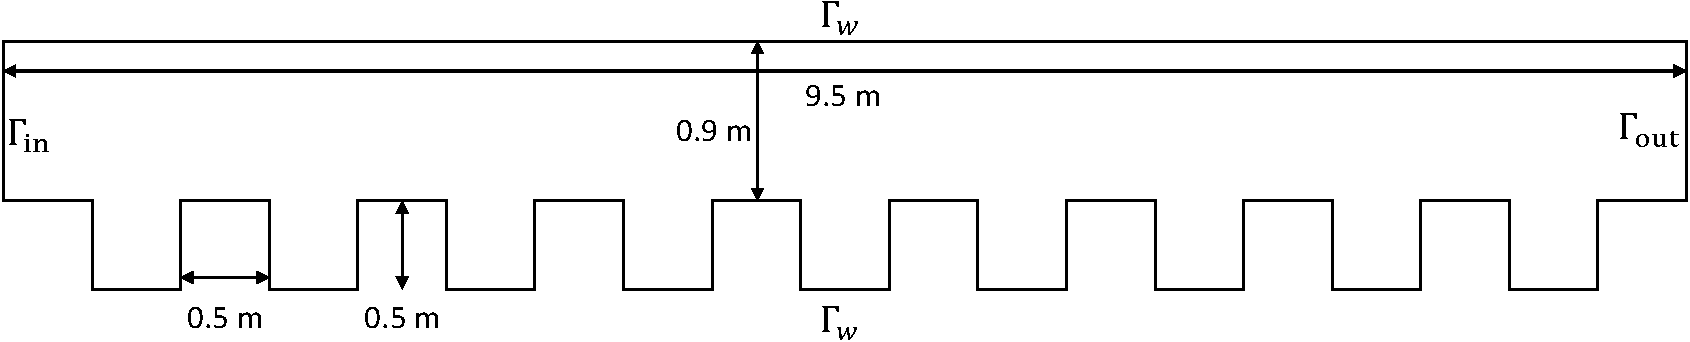
\includegraphics[width=\textwidth]{rough_domain_highstep2.pdf}
	\caption[Domain of the rough channel test with deep cavities]{Domain of the 
	rough channel test with deep cavities.}
	\label{fig:roughdomdeep}
\end{figure}
\begin{table}
	\centering
	\[
	\begin{array}{ccc}
	\toprule
	\text{Upwind} & \text{Van Leer} & \text{Van Alabada}\\
	\midrule
	\num{3.180e-4} & \num{5.862e-5} & \num{6.900e-5}\\
	\midrule
	\text{Min-Mod} & \text{Superbee} & \text{MC Limiter} \\
	\midrule
	\num{8.579e-5} & \num{7.883e-5} & \num{5.584e-5}\\
	\bottomrule
	\end{array}
	\]
	\caption[$L^2$-errors for the velocity in the rough channel with deep 
	cavities]{$L^2$-errors for the velocity along a section at $x=\SI{8.75}{m}$ 
	and $t=\SI{10}{s}$ in the rough channel with deep cavities. $Re = 
	\num{2e3}$.}
	\label{tab:errdeep}
\end{table}
\begin{figure}
	\centering
	% This file was created by matlab2tikz.
%
\definecolor{mycolor1}{rgb}{0.00000,0.44700,0.74100}%
\definecolor{mycolor2}{rgb}{0.85000,0.32500,0.09800}%
\definecolor{mycolor3}{rgb}{0.92900,0.69400,0.12500}%
\definecolor{mycolor4}{rgb}{0.49400,0.18400,0.55600}%
%
\begin{tikzpicture}

\begin{axis}[%
width=0.951\roughwidth,
height=0.75\roughheight,
at={(0\roughwidth,0\roughheight)},
scale only axis,
xmin=0,
xmax=1.4,
xlabel={$y$ [m]},
ymin=0,
ymax=1.25,
ylabel={Velocity magnitude [m/s]},
axis background/.style={fill=white},
legend style={at={(0.03,0.97)}, anchor=north west, legend cell align=left, align=left}
]

\addplot [color=mycolor1, mark size=1.5pt, mark=x, mark options={solid, mycolor1}, line width=0.75pt]
  table[row sep=crcr]{%
0	0\\
0.01	0.00885222\\
0.03	0.0227802\\
0.05	0.0327807\\
0.07	0.0393192\\
0.09	0.043122\\
0.11	0.0448784\\
0.13	0.0451341\\
0.15	0.0442874\\
0.17	0.0426208\\
0.19	0.0403378\\
0.21	0.037597\\
0.23	0.0345472\\
0.25	0.0313691\\
0.27	0.0283253\\
0.29	0.0258075\\
0.31	0.0243184\\
0.33	0.024277\\
0.35	0.0257093\\
0.37	0.0283224\\
0.39	0.0319839\\
0.41	0.0370173\\
0.43	0.044611\\
0.45	0.0576046\\
0.47	0.0818451\\
0.49	0.128213\\
0.51	0.214615\\
0.53	0.35431\\
0.55	0.509962\\
0.57	0.654372\\
0.59	0.77967\\
0.61	0.885193\\
0.63	0.971543\\
0.65	1.03985\\
0.67	1.0919\\
0.69	1.12994\\
0.71	1.15654\\
0.73	1.17426\\
0.75	1.18543\\
0.77	1.19201\\
0.79	1.19557\\
0.81	1.19723\\
0.83	1.1978\\
0.85	1.19779\\
0.87	1.19754\\
0.89	1.19723\\
0.91	1.19698\\
0.93	1.19685\\
0.95	1.19686\\
0.97	1.19703\\
0.99	1.19736\\
1.01	1.19783\\
1.03	1.19841\\
1.05	1.19906\\
1.07	1.19964\\
1.09	1.19992\\
1.11	1.19953\\
1.13	1.19783\\
1.15	1.19384\\
1.17	1.1861\\
1.19	1.17264\\
1.21	1.15086\\
1.23	1.11762\\
1.25	1.06938\\
1.27	1.00254\\
1.29	0.913831\\
1.31	0.800848\\
1.33	0.662508\\
1.35	0.499366\\
1.37	0.313659\\
1.39	0.109156\\
1.4	0\\
};
\addlegendentry{Upwind}

\addplot [color=mycolor2, mark size=1.5pt, mark=x, mark options={solid, mycolor2}, line width=0.75pt]
  table[row sep=crcr]{%
0	0\\
0.01	0.0122335\\
0.03	0.0324848\\
0.05	0.0480886\\
0.07	0.0588624\\
0.09	0.0654371\\
0.11	0.0686113\\
0.13	0.0688211\\
0.15	0.0669287\\
0.17	0.0627025\\
0.19	0.0563737\\
0.21	0.0484432\\
0.23	0.0398216\\
0.25	0.0319033\\
0.27	0.0265586\\
0.29	0.0256695\\
0.31	0.0288832\\
0.33	0.0340499\\
0.35	0.0396606\\
0.37	0.0450472\\
0.39	0.0499693\\
0.41	0.0545328\\
0.43	0.0595794\\
0.45	0.0677895\\
0.47	0.0859627\\
0.49	0.128135\\
0.51	0.214164\\
0.53	0.35562\\
0.55	0.519342\\
0.57	0.670222\\
0.59	0.798895\\
0.61	0.905422\\
0.63	0.991025\\
0.65	1.05726\\
0.67	1.10635\\
0.69	1.14101\\
0.71	1.16412\\
0.73	1.17855\\
0.75	1.18688\\
0.77	1.19113\\
0.79	1.19289\\
0.81	1.19325\\
0.83	1.1929\\
0.85	1.19227\\
0.87	1.19163\\
0.89	1.19106\\
0.91	1.19067\\
0.93	1.19044\\
0.95	1.19037\\
0.97	1.1905\\
0.99	1.19084\\
1.01	1.19135\\
1.03	1.19204\\
1.05	1.19284\\
1.07	1.19365\\
1.09	1.19427\\
1.11	1.19434\\
1.13	1.19322\\
1.15	1.1899\\
1.17	1.18285\\
1.19	1.16996\\
1.21	1.14851\\
1.23	1.11525\\
1.25	1.06662\\
1.27	0.999152\\
1.29	0.909811\\
1.31	0.796478\\
1.33	0.658286\\
1.35	0.495815\\
1.37	0.311267\\
1.39	0.108298\\
1.4	0\\
};
\addlegendentry{Van Leer}

\addplot [color=mycolor3, mark size=1.5pt, mark=x, mark options={solid, mycolor3}, line width=0.75pt]
  table[row sep=crcr]{%
0	0\\
0.01	0.0113419\\
0.03	0.0297822\\
0.05	0.0438459\\
0.07	0.0535293\\
0.09	0.0594514\\
0.11	0.0623285\\
0.13	0.0627341\\
0.15	0.0613312\\
0.17	0.0581295\\
0.19	0.0533229\\
0.21	0.0472654\\
0.23	0.040544\\
0.25	0.0340756\\
0.27	0.0291588\\
0.29	0.0272168\\
0.31	0.0284915\\
0.33	0.0317763\\
0.35	0.0359173\\
0.37	0.0402998\\
0.39	0.0446982\\
0.41	0.0493064\\
0.43	0.0551453\\
0.45	0.0648297\\
0.47	0.0848545\\
0.49	0.128268\\
0.51	0.214524\\
0.53	0.355773\\
0.55	0.518594\\
0.57	0.668691\\
0.59	0.796856\\
0.61	0.903066\\
0.63	0.988544\\
0.65	1.05485\\
0.67	1.10418\\
0.69	1.13918\\
0.71	1.16273\\
0.73	1.17764\\
0.75	1.1864\\
0.77	1.19104\\
0.79	1.19311\\
0.81	1.19369\\
0.83	1.19352\\
0.85	1.19301\\
0.87	1.19243\\
0.89	1.19193\\
0.91	1.19158\\
0.93	1.19138\\
0.95	1.19133\\
0.97	1.19148\\
0.99	1.19181\\
1.01	1.19232\\
1.03	1.19298\\
1.05	1.19375\\
1.07	1.19452\\
1.09	1.19508\\
1.11	1.19505\\
1.13	1.19379\\
1.15	1.1903\\
1.17	1.18309\\
1.19	1.17005\\
1.21	1.14852\\
1.23	1.11526\\
1.25	1.06673\\
1.27	0.999415\\
1.29	0.910241\\
1.31	0.797042\\
1.33	0.658892\\
1.35	0.496348\\
1.37	0.311635\\
1.39	0.108434\\
1.4	0\\
};
\addlegendentry{Min-Mod}

\addplot [color=mycolor4, line width=0.75pt]
  table[row sep=crcr]{%
0	0\\
0.00166667	0.00162965\\
0.005	0.00480799\\
0.00833333	0.00790634\\
0.0116667	0.0109252\\
0.015	0.013865\\
0.0183333	0.0167258\\
0.0216667	0.019508\\
0.025	0.022212\\
0.0283333	0.0248383\\
0.0316667	0.0273878\\
0.035	0.0298613\\
0.0383333	0.03226\\
0.0416667	0.0345853\\
0.045	0.0368385\\
0.0483333	0.0390211\\
0.0516667	0.0411348\\
0.055	0.0431809\\
0.0583333	0.045161\\
0.0616667	0.0470764\\
0.065	0.0489283\\
0.0683333	0.0507176\\
0.0716667	0.0524452\\
0.075	0.0541115\\
0.0783333	0.055717\\
0.0816667	0.0572619\\
0.085	0.0587457\\
0.0883333	0.0601683\\
0.0916667	0.0615291\\
0.095	0.0628271\\
0.0983333	0.0640617\\
0.101667	0.0652316\\
0.105	0.0663357\\
0.108333	0.0673728\\
0.111667	0.0683414\\
0.115	0.0692403\\
0.118333	0.070068\\
0.121667	0.0708231\\
0.125	0.0715044\\
0.128333	0.0721104\\
0.131667	0.0726401\\
0.135	0.0730923\\
0.138333	0.0734658\\
0.141667	0.0737601\\
0.145	0.0739741\\
0.148333	0.0741073\\
0.151667	0.0741594\\
0.155	0.0741298\\
0.158333	0.0740188\\
0.161667	0.0738262\\
0.165	0.0735523\\
0.168333	0.0731975\\
0.171667	0.0727624\\
0.175	0.0722478\\
0.178333	0.0716544\\
0.181667	0.0709837\\
0.185	0.0702367\\
0.188333	0.0694149\\
0.191667	0.0685199\\
0.195	0.0675533\\
0.198333	0.0665172\\
0.201667	0.0654135\\
0.205	0.0642444\\
0.208333	0.0630124\\
0.211667	0.0617197\\
0.215	0.0603692\\
0.218333	0.0589636\\
0.221667	0.0575058\\
0.225	0.055999\\
0.228333	0.0544466\\
0.231667	0.0528522\\
0.235	0.0512197\\
0.238333	0.0495534\\
0.241667	0.0478579\\
0.245	0.0461384\\
0.248333	0.0444006\\
0.251667	0.042651\\
0.255	0.0408971\\
0.258333	0.0391474\\
0.261667	0.0374118\\
0.265	0.0357016\\
0.268333	0.0340304\\
0.271667	0.032414\\
0.275	0.0308707\\
0.278333	0.0294217\\
0.281667	0.0280915\\
0.285	0.026907\\
0.288333	0.025897\\
0.291667	0.0250911\\
0.295	0.0245166\\
0.298333	0.0241958\\
0.301667	0.0241434\\
0.305	0.024363\\
0.308333	0.0248475\\
0.311667	0.0255795\\
0.315	0.0265348\\
0.318333	0.0276856\\
0.321667	0.0290029\\
0.325	0.0304586\\
0.328333	0.0320267\\
0.331667	0.0336841\\
0.335	0.0354105\\
0.338333	0.0371883\\
0.341667	0.0390024\\
0.345	0.0408399\\
0.348333	0.0426898\\
0.351667	0.0445425\\
0.355	0.04639\\
0.358333	0.048225\\
0.361667	0.0500416\\
0.365	0.0518343\\
0.368333	0.0535986\\
0.371667	0.0553303\\
0.375	0.0570259\\
0.378333	0.0586824\\
0.381667	0.060297\\
0.385	0.0618676\\
0.388333	0.0633923\\
0.391667	0.0648697\\
0.395	0.0662986\\
0.398333	0.0676785\\
0.401667	0.0690093\\
0.405	0.0702916\\
0.408333	0.0715265\\
0.411667	0.072716\\
0.415	0.0738628\\
0.418333	0.0749713\\
0.421667	0.076047\\
0.425	0.0770969\\
0.428333	0.0781306\\
0.431667	0.0791597\\
0.435	0.0801992\\
0.438333	0.0812674\\
0.441667	0.0823869\\
0.445	0.0835853\\
0.448333	0.084896\\
0.451667	0.0863585\\
0.455	0.08802\\
0.458333	0.0899355\\
0.461667	0.0921692\\
0.465	0.0947941\\
0.468333	0.0978929\\
0.471667	0.101558\\
0.475	0.105891\\
0.478333	0.111\\
0.481667	0.117001\\
0.485	0.124015\\
0.488333	0.13216\\
0.491667	0.141554\\
0.495	0.152307\\
0.498333	0.164518\\
0.501667	0.178267\\
0.505	0.193612\\
0.508333	0.210581\\
0.511667	0.229172\\
0.515	0.249346\\
0.518333	0.271026\\
0.521667	0.294097\\
0.525	0.318416\\
0.528333	0.3438\\
0.531667	0.370031\\
0.535	0.396864\\
0.538333	0.42408\\
0.541667	0.451482\\
0.545	0.478885\\
0.548333	0.506133\\
0.551667	0.533085\\
0.555	0.559629\\
0.558333	0.585678\\
0.561667	0.611162\\
0.565	0.636036\\
0.568333	0.660269\\
0.571667	0.683845\\
0.575	0.706758\\
0.578333	0.729008\\
0.581667	0.750601\\
0.585	0.771545\\
0.588333	0.79185\\
0.591667	0.811525\\
0.595	0.83058\\
0.598333	0.849024\\
0.601667	0.866863\\
0.605	0.884107\\
0.608333	0.900759\\
0.611667	0.916826\\
0.615	0.932313\\
0.618333	0.947225\\
0.621667	0.961569\\
0.625	0.975348\\
0.628333	0.988573\\
0.631667	1.00125\\
0.635	1.01338\\
0.638333	1.02498\\
0.641667	1.03605\\
0.645	1.04661\\
0.648333	1.05667\\
0.651667	1.06623\\
0.655	1.07531\\
0.658333	1.08392\\
0.661667	1.09207\\
0.665	1.09978\\
0.668333	1.10705\\
0.671667	1.11391\\
0.675	1.12035\\
0.678333	1.12641\\
0.681667	1.13209\\
0.685	1.1374\\
0.688333	1.14237\\
0.691667	1.147\\
0.695	1.15131\\
0.698333	1.15531\\
0.701667	1.15901\\
0.705	1.16244\\
0.708333	1.1656\\
0.711667	1.16851\\
0.715	1.17118\\
0.718333	1.17363\\
0.721667	1.17586\\
0.725	1.17789\\
0.728333	1.17974\\
0.731667	1.18141\\
0.735	1.18291\\
0.738333	1.18425\\
0.741667	1.18546\\
0.745	1.18653\\
0.748333	1.18747\\
0.751667	1.18831\\
0.755	1.18903\\
0.758333	1.18966\\
0.761667	1.1902\\
0.765	1.19066\\
0.768333	1.19104\\
0.771667	1.19135\\
0.775	1.19161\\
0.778333	1.19181\\
0.781667	1.19195\\
0.785	1.19206\\
0.788333	1.19212\\
0.791667	1.19214\\
0.795	1.19214\\
0.798333	1.19211\\
0.801667	1.19205\\
0.805	1.19197\\
0.808333	1.19188\\
0.811667	1.19177\\
0.815	1.19164\\
0.818333	1.19151\\
0.821667	1.19136\\
0.825	1.19121\\
0.828333	1.19106\\
0.831667	1.1909\\
0.835	1.19073\\
0.838333	1.19057\\
0.841667	1.19041\\
0.845	1.19025\\
0.848333	1.19009\\
0.851667	1.18993\\
0.855	1.18977\\
0.858333	1.18962\\
0.861667	1.18947\\
0.865	1.18933\\
0.868333	1.18919\\
0.871667	1.18906\\
0.875	1.18893\\
0.878333	1.18881\\
0.881667	1.18869\\
0.885	1.18858\\
0.888333	1.18847\\
0.891667	1.18838\\
0.895	1.18828\\
0.898333	1.1882\\
0.901667	1.18812\\
0.905	1.18804\\
0.908333	1.18797\\
0.911667	1.18791\\
0.915	1.18786\\
0.918333	1.18781\\
0.921667	1.18776\\
0.925	1.18773\\
0.928333	1.1877\\
0.931667	1.18767\\
0.935	1.18765\\
0.938333	1.18764\\
0.941667	1.18763\\
0.945	1.18763\\
0.948333	1.18764\\
0.951667	1.18765\\
0.955	1.18767\\
0.958333	1.18769\\
0.961667	1.18772\\
0.965	1.18776\\
0.968333	1.1878\\
0.971667	1.18785\\
0.975	1.1879\\
0.978333	1.18797\\
0.981667	1.18803\\
0.985	1.18811\\
0.988333	1.18818\\
0.991667	1.18827\\
0.995	1.18836\\
0.998333	1.18846\\
1.00167	1.18856\\
1.005	1.18867\\
1.00833	1.18879\\
1.01167	1.18891\\
1.015	1.18904\\
1.01833	1.18917\\
1.02167	1.18931\\
1.025	1.18946\\
1.02833	1.18961\\
1.03167	1.18977\\
1.035	1.18993\\
1.03833	1.1901\\
1.04167	1.19027\\
1.045	1.19045\\
1.04833	1.19063\\
1.05167	1.19081\\
1.055	1.191\\
1.05833	1.19119\\
1.06167	1.19139\\
1.065	1.19158\\
1.06833	1.19177\\
1.07167	1.19197\\
1.075	1.19216\\
1.07833	1.19235\\
1.08167	1.19253\\
1.085	1.19271\\
1.08833	1.19288\\
1.09167	1.19305\\
1.095	1.1932\\
1.09833	1.19333\\
1.10167	1.19345\\
1.105	1.19355\\
1.10833	1.19362\\
1.11167	1.19367\\
1.115	1.19369\\
1.11833	1.19368\\
1.12167	1.19363\\
1.125	1.19353\\
1.12833	1.19338\\
1.13167	1.19319\\
1.135	1.19293\\
1.13833	1.1926\\
1.14167	1.1922\\
1.145	1.19172\\
1.14833	1.19115\\
1.15167	1.19049\\
1.155	1.18971\\
1.15833	1.18883\\
1.16167	1.18782\\
1.165	1.18667\\
1.16833	1.18538\\
1.17167	1.18393\\
1.175	1.18231\\
1.17833	1.18051\\
1.18167	1.17852\\
1.185	1.17632\\
1.18833	1.17389\\
1.19167	1.17123\\
1.195	1.16832\\
1.19833	1.16515\\
1.20167	1.1617\\
1.205	1.15794\\
1.20833	1.15388\\
1.21167	1.14949\\
1.215	1.14475\\
1.21833	1.13965\\
1.22167	1.13417\\
1.225	1.12829\\
1.22833	1.12201\\
1.23167	1.11529\\
1.235	1.10812\\
1.23833	1.1005\\
1.24167	1.09239\\
1.245	1.08378\\
1.24833	1.07466\\
1.25167	1.06502\\
1.255	1.05483\\
1.25833	1.04408\\
1.26167	1.03276\\
1.265	1.02085\\
1.26833	1.00835\\
1.27167	0.995228\\
1.275	0.981485\\
1.27833	0.967108\\
1.28167	0.952085\\
1.285	0.936409\\
1.28833	0.92007\\
1.29167	0.903062\\
1.295	0.885377\\
1.29833	0.867011\\
1.30167	0.847959\\
1.305	0.828218\\
1.30833	0.807786\\
1.31167	0.786662\\
1.315	0.764846\\
1.31833	0.742339\\
1.32167	0.719144\\
1.325	0.695264\\
1.32833	0.670704\\
1.33167	0.645471\\
1.335	0.619571\\
1.33833	0.593012\\
1.34167	0.565805\\
1.345	0.537959\\
1.34833	0.509487\\
1.35167	0.480401\\
1.355	0.450714\\
1.35833	0.420443\\
1.36167	0.389601\\
1.365	0.358207\\
1.36833	0.326277\\
1.37167	0.29383\\
1.375	0.260885\\
1.37833	0.227463\\
1.38167	0.193583\\
1.385	0.159268\\
1.38833	0.124538\\
1.39167	0.0894149\\
1.395	0.0539223\\
1.39833	0.0180823\\
1.4	0\\
};
\addlegendentry{Reference}
\addplot [color=black, dashed, line width=0.75pt]
  table[row sep=crcr]{%
0.5	0\\
0.5 1.25\\
};
\end{axis}
\end{tikzpicture}%
	\caption[short text]{text}
	\label{fig:linecompdeep}
\end{figure}
%
\section{RANS tests}
\subsection{Backward facing step}
%The NASA LaRC CFD code CFL3D uses:
%\begin{itemize}
%	\item free-stream turbulence intensity = 0.061\%
%	\item free-stream turbulent viscosity (relative to laminar) = 0.009
%	\item in this case the simulations were \emph{quasi-steady}, i.e. the 
%	solution does not converge readily to a steady state result when a refined 
%	grid is used. However, when run-time accurately, the solution settles down 
%	and becomes reasonably steady (quasi-steady).
%	\item The code is for compressible flows at ``essentially incompressible" 
%	conditions of M=0.128. There may be a very small influence of 
%	compressibility.
%	\item non-dimensional CFD code
%	\item first order turbulence advection in the turbulence transport equations
%	\item Neglects two terms that are zero for incompressible flows
%	\item implicit time advancement (also second order)
%	\item Central differencing in Space? Non lo dice cosa usa, inoltre secondo 
%	me non usa una staggered grid.
%\end{itemize}
\subsection{Cavities mutual influence}
%An easy result.
\section{Coupled test}
\subsection{Cavities coupled with the porous-medium}
%A more complex result.
\chapter{Conclusions and outlook}
\section{Conclusions}
In this work we have seen the application of the TVD methods for the 
approximation of the convective term in the momentum equation of the 
Navier-Stokes equations and of the RANS equations, within a finite volumes 
framework. The aim was to use them for the simulation of coupled free-flow and 
porous-medium flow models, improving the results obtained employing the 
first order upwind scheme, using a method that introduces less numerical 
viscosity in the solution, but that, at the same time, guarantees the stability 
and avoids the creation of unphysical oscillations.

In all the tests that have been performed, we have experienced an increased 
accuracy of the solution with respect to those obtained when using the first order 
upwind method. The spatial convergence rates in the tests with analytical 
solution were between 1.5 and 2 in many cases, while with the upwind method we had always a first order convergence. 
The differences were more relevant at $Re\simeq\num{e3}$ rather than at 
$Re\simeq1$, because of the increased importance of the convective term with 
respect to the diffusive one. Also with turbulent flows in the backward facing 
step test, we have 
obtained, using the Van Leer flux limiter, a satisfying agreement with 
validated numerical results from the CFL3D code and experimental data.
Moreover, employing a BDF2 scheme for the 
temporal discretization, we have available an high order discretization both 
in space and in time, thus allowing a more accurate study of transient 
phenomena.

With this tool, we have studied a coupled model made of a free-flow and a 
porous-medium flow, focusing in particular on the effects that a rough
interface, with cavities or porous obstacles, has on the flow field.

At first, we have considered only the free-flow and we have studied how the 
velocity is affected by the presence of two cavities at the interface.
In particular, we have investigated which is the distance between the cavities such that the variation in the flow field, 
because of the first cavity, does not significantly influence anymore the 
behaviour around the 
second one. We have obtained that, for cavities $\SI{0.5}{m}$ long, after a 
distance equal to one cavity the flow field has recovered the configuration it 
had before the first cavity. However each cavity introduces an increase in the 
turbulent kinetic energy, that accelerates the growth of the turbulent 
boundary layer.

Afterwards we have chosen a distance such that the two cavities do not 
influence each other and we have placed a porous-medium between them, in order 
to analyse how its presence affects the flow field. We have observed that, 
for values of permeability greater than $\SI{e-8}{m^2}$, the flow field in the 
free-flow shows noticeable differences when compared to a case without a 
porous-medium, both in the case of the shallow cavities and deep cavities.
In particular, not only the fact that the flow can enter into 
the porous-medium has an effect, but also the Beaver-Joseph-Saffman slip 
condition that was imposed at the interface between the two subdomains affects the flow dynamics.
The presence of eddies in the cavities influences the flow in the 
porous-medium, because in correspondence of the corner eddies it can enter also 
from a direction opposite to the one of the main flow. However, when this 
happens, the values of the velocity are relatively small and thus this 
behaviour does not affect the free-flow as it happens when the flow enters the 
porous-medium at the end of a cavity. We have evaluated the mass flow 
rate from the free-flow region to the porous-medium and we have noticed a 
relevant 
increase for values of permeability greater than $\SI{e-8}{m^2}$. Comparing 
the cases of shallow and deep cavities, the mass flow rate has shown to be 
proportional to the measure of the interface.

At last, we have considered a flow in a channel with a porous obstacles on the 
lower boundary. We have observed that the porous-medium flow influences the 
free-flow only at the frontal face of the obstacle, where the flow is stopped 
by the porous medium, while at the backward face the behaviour remains the same 
independently of the permeability.
%
\section{Future developments}
Future developments to this thesis can be devoted to the investigation of more 
complex models, involving multiphase, multi-component and non-isothermal 
models. Exploiting the accuracy of high-resolution methods, a more reliable 
prediction of the evaporation rate from a wet soil could be performed. 
Moreover, it could be interesting to study other types of \emph{rough} 
interfaces, for example to see if a smooth interface described by a sinusoidal 
function could behave differently with respect to those we have analysed.

In this work the TVD methods have been adopted only in the momentum equation, 
but, in particular with non-isothermal models with non-constant density, from 
the numerical point of view it could be important to analyse their 
application to the continuity equation.

From the point of view of the coupling, the interface conditions could be adapted in order to employ other finite volumes discretization schemes in the porous-medium, including, for example, a Multi Point Flux Approximation (MPFA).
Moreover, iterative algorithms to decouple the two subdomains could be taken 
into account and compared to the monolithic approach we have used.

Within the \DUMUX framework a possibility to improve the feasibility of the 
simulations could be to employ an adaptive algorithm in order to refine the grid 
only where it is useful. This approach can lead to non-conforming meshes 
containing hanging nodes, thus a challenge would be the application of the TVD 
scheme to this case. Moreover a parallelization of the code would be 
beneficial for the computational time, but the extended stencil of high order methods 
requires attention whilst decomposing the domain.
\appendix
\renewcommand{\chaptername}{Appendix}
\chapter{Space convergence} \label{app:conv}
We report here some more convergence examples in addition to the Sin-Cos 
presented in Subsection~\ref{subsec:conv}.
%
\section{1D test}
We solve the equations~\eqref{eq:nssteadymass}--\eqref{eq:nssteadymom} over a 
one-dimensional unit domain $\Omega=(0,1)$, with the following source terms:
\begin{align}
	h &= 6x^2,\\
	f &= 12x^5 - 24\nu x - \frac{2}{\varrho} % con enableUnsymmetrizedGradient
\end{align}
so that, choosing $\varrho=1$, the analytical solution, depicted in 
Figure~\ref{fig:1dexact}, is given by
\begin{align}
\label{eq:uex1d}	u_\text{ex}(x) &= 2x^3\\
\label{eq:pex1d}	p_\text{ex}(x) &= 2-2x
\end{align}
Dirichlet boundary conditions for the velocity are applied on the whole 
boundary $\partial \Omega$ using the exact solution. The pressure is fixed at 
one point in order to match the exact solution \eqref{eq:pex1d}.
\begin{figure}
	\centering
	\begin{tikzpicture}
	\begin{axis}[width=0.47\textwidth, xlabel={$x$}, xmin=0, xmax=1, ymin=0, 
	ymax=2,	samples=100, ylabel={$u_\text{ex}$}, ylabel style={rotate=-90}]
	\addplot[color=black, mark=none, line width=1.0pt]{2*x*x};
	\end{axis}
	\end{tikzpicture}
%	\hskip 5pt
	\begin{tikzpicture}
	\begin{axis}[width=0.47\textwidth, xlabel={$x$}, xmin=0, xmax=1, ymin=0, 
	ymax=2, samples=100, 
	ylabel={$p_\text{ex}$}, ylabel style={rotate=-90}]
	\addplot[color=black, mark=none, line width=1.0pt]{2*(1-x)};
	\end{axis}
	\end{tikzpicture}
	\caption[Exact solution of the 1D test]{Exact solution of the 1D test 
	\eqref{eq:uex1d}--\eqref{eq:pex1d}. On 
	the left the velocity field, on the right the pressure field.}
	\label{fig:1dexact}
\end{figure}

The problem is solved over a sequence of eight uniform grids, starting from 
4 cells and each time halving their size. Both the cases of $\nu=1$ 
and $\nu=\num{e-3}$ are considered, that correspond respectively to $Re=1$ and $Re=\num{e3}$. In Figure~\ref{fig:1d_err} the errors computed are reported 
depending on the number of cells, while in 
Table~\ref{tab:1d} we can compare directly the 
convergence orders for the different differencing schemes.
\begin{figure}
	\centering
	\subfloat[Upwind, $Re = 1$]{
		% This file was created by matlab2tikz.
%
\definecolor{mycolor1}{rgb}{0.00000,0.44700,0.74100}%
\definecolor{mycolor2}{rgb}{0.85000,0.32500,0.09800}%
%
\begin{tikzpicture}

\begin{axis}[%
width=0.951\figwidth,
height=0.75\figwidth,
at={(0\figwidth,0\figwidth)},
scale only axis,
xmode=log,
xmin=4,
xmax=1000,
xminorticks=true,
ymode=log,
ymin=1e-06,
ymax=1,
yminorticks=true,
axis background/.style={fill=white},
legend style={at={(0.03,0.03)}, anchor=south west, legend cell align=left, align=left}
]
\addplot [color=white!70!black, forget plot, line width=0.75pt]
  table[row sep=crcr]{%
4	0.00025\\
1000	1e-06\\
};
\addplot [color=white!70!black, forget plot, line width=0.75pt]
  table[row sep=crcr]{%
4	0.0625\\
1000	1e-06\\
};
\addplot [color=mycolor1, mark=x, mark options={solid, mycolor1}, line width=0.75pt]
  table[row sep=crcr]{%
4	0.214116295\\
8	0.195589151\\
16	0.132868874\\
32	0.0777359686\\
64	0.0420904681\\
128	0.0219065573\\
256	0.011175991\\
512	0.00564462389\\
};
\addlegendentry{$p$}

\addplot [color=mycolor2, mark=x, mark options={solid, mycolor2}, line width=0.75pt]
  table[row sep=crcr]
	\subfloat[Upwind, $Re = \num{e3}$]{
		% This file was created by matlab2tikz.
%
\definecolor{mycolor1}{rgb}{0.00000,0.44700,0.74100}%
\definecolor{mycolor2}{rgb}{0.85000,0.32500,0.09800}%
%
\begin{tikzpicture}

\begin{axis}[%
width=0.951\figwidth,
height=0.75\figwidth,
at={(0\figwidth,0\figwidth)},
scale only axis,
xmode=log,
xmin=4,
xmax=1000,
xminorticks=true,
ymode=log,
ymin=0.001,
ymax=0.190700916,
yminorticks=true,
axis background/.style={fill=white},
legend style={at={(0.03,0.03)}, anchor=south west, legend cell align=left, align=left}
]
\addplot [color=mycolor1, mark=x, mark options={solid, mycolor1}]
  table[row sep=crcr]{%
4	0.0950934111\\
8	0.0956441228\\
16	0.0633456286\\
32	0.0359064412\\
64	0.0189587968\\
128	0.009733956\\
256	0.00507474159\\
512	0.00281243348\\
};
\addlegendentry{$p$}

\addplot [color=mycolor2, mark=x, mark options={solid, mycolor2}]
  table[row sep=crcr]{%
4	0.190700916\\
8	0.161981022\\
16	0.100050412\\
32	0.0542847205\\
64	0.0273944361\\
128	0.013011169\\
256	0.00574729458\\
512	0.00230500508\\
};
\addlegendentry{$u$}

\addplot [color=white!70!black, forget plot]
  table[row sep=crcr]{%
4	0.25\\
1000	0.001\\
};
\addplot [color=white!70!black, forget plot]
  table[row sep=crcr]\\
	\subfloat[Min-Mod, $Re = 1$]{
		% This file was created by matlab2tikz.
%
\definecolor{mycolor1}{rgb}{0.00000,0.44700,0.74100}%
\definecolor{mycolor2}{rgb}{0.85000,0.32500,0.09800}%
%
\begin{tikzpicture}

\begin{axis}[%
width=0.951\figwidth,
height=0.75\figwidth,
at={(0\figwidth,0\figwidth)},
scale only axis,
xmode=log,
xmin=4,
xmax=1000,
xminorticks=true,
ymode=log,
ymin=1e-07,
ymax=0.1,
yminorticks=true,
axis background/.style={fill=white},
legend style={at={(0.03,0.03)}, anchor=south west, legend cell align=left, align=left}
]
\addplot [color=mycolor1, mark=x, mark options={solid, mycolor1}]
  table[row sep=crcr]{%
4	0.0947400829\\
8	0.0579455977\\
16	0.0306653228\\
32	0.0155606681\\
64	0.00780733847\\
128	0.00390635907\\
256	0.0019533289\\
512	0.000976635645\\
};
\addlegendentry{$p$}

\addplot [color=mycolor2, mark=x, mark options={solid, mycolor2}]
  table[row sep=crcr]{%
4	0.00558067417\\
8	0.00185644832\\
16	0.000515125253\\
32	0.000134752887\\
64	3.44440641e-05\\
128	8.70859755e-06\\
256	2.18965445e-06\\
512	5.49000176e-07\\
};
\addlegendentry{$u$}

\addplot [color=white!70!black, forget plot]
  table[row sep=crcr]{%
4	2.5e-05\\
1000	1e-07\\
};
\addplot [color=white!70!black, forget plot]
  table[row sep=crcr]
	\subfloat[Min-Mod, $Re = \num{e3}$]{
		% This file was created by matlab2tikz.
%
\definecolor{mycolor1}{rgb}{0.00000,0.44700,0.74100}%
\definecolor{mycolor2}{rgb}{0.85000,0.32500,0.09800}%
%
\begin{tikzpicture}

\begin{axis}[%
width=0.951\figwidth,
height=0.75\figwidth,
at={(0\figwidth,0\figwidth)},
scale only axis,
xmode=log,
xmin=4,
xmax=1000,
xminorticks=true,
ymode=log,
ymin=1e-06,
ymax=0.01,
yminorticks=true,
axis background/.style={fill=white},
legend style={at={(0.03,0.03)}, anchor=south west, legend cell align=left, align=left}
]
\addplot [color=mycolor1, mark=x, mark options={solid, mycolor1}]
  table[row sep=crcr]{%
4	0.0044619081\\
8	0.00229663251\\
16	0.000841546306\\
32	0.000255627656\\
64	7.28671934e-05\\
128	2.11819043e-05\\
256	6.7259867e-06\\
512	2.37553605e-06\\
};
\addlegendentry{$p$}

\addplot [color=mycolor2, mark=x, mark options={solid, mycolor2}]
  table[row sep=crcr]{%
4	0.00900152872\\
8	0.00490327033\\
16	0.0016983622\\
32	0.000486317571\\
64	0.00012618377\\
128	3.05074557e-05\\
256	6.86153125e-06\\
512	1.41905971e-06\\
};
\addlegendentry{$u$}

\addplot [color=white!70!black, forget plot]
  table[row sep=crcr]{%
4	0.00025\\
1000	1e-06\\
};
\addplot [color=white!70!black, forget plot]
  table[row sep=crcr]\\
	\subfloat[Van Leer, $Re = 1$]{
		% This file was created by matlab2tikz.
%
\definecolor{mycolor1}{rgb}{0.00000,0.44700,0.74100}%
\definecolor{mycolor2}{rgb}{0.85000,0.32500,0.09800}%
%
\begin{tikzpicture}

\begin{axis}[%
width=0.951\figwidth,
height=0.75\figwidth,
at={(0\figwidth,0\figwidth)},
scale only axis,
xmode=log,
xmin=4,
xmax=1000,
xminorticks=true,
ymode=log,
ymin=1e-07,
ymax=0.1,
yminorticks=true,
axis background/.style={fill=white},
legend style={at={(0.03,0.03)}, anchor=south west, legend cell align=left, align=left}
]
\addplot [color=mycolor1, mark=x, mark options={solid, mycolor1}]
  table[row sep=crcr]{%
4	0.058505198\\
8	0.0412346964\\
16	0.0251402529\\
32	0.0139748536\\
64	0.00738268213\\
128	0.00379649657\\
256	0.00192539001\\
512	0.000969591076\\
};
\addlegendentry{$p$}

\addplot [color=mycolor2, mark=x, mark options={solid, mycolor2}]
  table[row sep=crcr]{%
4	0.00804947871\\
8	0.0022466016\\
16	0.0005523443\\
32	0.000137569802\\
64	3.46360203e-05\\
128	8.7210858e-06\\
256	2.19045006e-06\\
512	5.49050369e-07\\
};
\addlegendentry{$u$}

\addplot [color=white!70!black, forget plot]
  table[row sep=crcr]{%
4	2.5e-05\\
1000	1e-07\\
};
\addplot [color=white!70!black, forget plot]
  table[row sep=crcr]
	\subfloat[Van Leer, $Re = \num{e3}$]{
		% This file was created by matlab2tikz.
%
\definecolor{mycolor1}{rgb}{0.00000,0.44700,0.74100}%
\definecolor{mycolor2}{rgb}{0.85000,0.32500,0.09800}%
%
\begin{tikzpicture}

\begin{axis}[%
width=0.951\figwidth,
height=0.75\figwidth,
at={(0\figwidth,0\figwidth)},
scale only axis,
xmode=log,
xmin=4,
xmax=1000,
xminorticks=true,
ymode=log,
ymin=1e-06,
ymax=0.1,
yminorticks=true,
axis background/.style={fill=white},
legend style={at={(0.03,0.03)}, anchor=south west, legend cell align=left, align=left, draw=white!15!black}
]
\addplot [color=mycolor1, mark=x, mark options={solid, mycolor1}]
  table[row sep=crcr]{%
4	0.0161844304\\
8	0.00984258579\\
16	0.00351641157\\
32	0.00101607975\\
64	0.000263342669\\
128	6.34168067e-05\\
256	1.44388667e-05\\
512	3.20413694e-06\\
};
\addlegendentry{$p$}

\addplot [color=mycolor2, mark=x, mark options={solid, mycolor2}]
  table[row sep=crcr]{%
4	0.0562254093\\
8	0.020321909\\
16	0.00583980329\\
32	0.0015266502\\
64	0.000376324406\\
128	8.75670102e-05\\
256	1.88988619e-05\\
512	3.69275832e-06\\
};
\addlegendentry{$u$}

\addplot [color=white!70!black, forget plot]
  table[row sep=crcr]{%
4	0.00025\\
1000	1e-06\\
};
\addplot [color=white!70!black, forget plot]
  table[row sep=crcr]
	\caption[$L^2(\Omega)$ norm of the errors for the 1D test]{$L^2(\Omega)$ 
	norm of the errors for the 1D test 
	depending on the number of cells in the grid. The grey lines are the 
	reference lines for the first-order (lower) and second-order (upper) 
	convergence.}
	\label{fig:1d_err}
\end{figure}
\begin{table}
	\centering
	\subfloat[$Re=1$]{
	$\begin{array}{c|ccc}
	\toprule
	& \text{Upwind} & \text{Min-Mod} & \text{Van Leer} \\ 
	\midrule
	p & 0.985 & 1.000 & 0.990\\
	u & 1.985 & 1.996 & 1.996\\
	\bottomrule
	\end{array}
	\label{tab:1d_lre}$
	}\\
	\subfloat[$Re=\num{e3}$]{
	$\begin{array}{c|ccc}
	\toprule
	& \text{Upwind} & \text{Min-Mod} & \text{Van Leer} \\ 
	\midrule
	p & 0.852 & 1.501 & 2.172\\
	u & 1.318 & 2.274 & 2.356\\
	\bottomrule
	\end{array}
	\label{tab:1d_hre}$}
	\caption[Convergence orders for the 1D 
	test]{Convergence orders with for the 1D test. They 
	are computed considering the last two refinements of the grid.}
	\label{tab:1d}
\end{table}

In this test, at $Re=1$, all the methods behave similarly, as we 
can see in Table~\ref{tab:1d_lre}, with the second-order convergence for the 
velocity also using the upwind method. Probably, in this one-dimensional 
configuration, the second-order diffusive term is dominating. From 
Table~\ref{tab:1d_hre} we observe instead that the TVD methods keep the second-order 
convergence for the velocity and increase the rate also for the pressure, while 
the upwind method decreases them. With the finest grid we observe from 
Figure~\ref{fig:1d_err} that with the TVD methods the errors are three orders of 
magnitude lower than with the upwind method.

%\FloatBarrier
%
\section{Kovasznay test}
We solve the equations~\eqref{eq:nssteadymass}--\eqref{eq:nssteadymom} over a 
two-dimensional domain $\Omega=(-0.5, 2) \times (-0.5,1.5)$, without any source 
term, so that, choosing $\varrho=1$, the analytical solution, depicted in 
Figure~\ref{fig:kovexact}, is given by
\begin{align}
\label{eq:uexkov} u_\text{ex}(x,y) &= 1-e^{\lambda x} \cos (2 \pi y)\\
v_\text{ex}(x,y) &= \frac{\lambda}{2\pi} e^{\lambda x} \sin (2\pi y)\\
\label{eq:pexkov}	p_\text{ex}(x,y) &= \frac{1}{2}(1 -e^{2\lambda x})\\
\lambda &= \frac{1}{2 \nu} - \sqrt{\frac{1}{4 \nu^2} + 4\pi^2},
\end{align}
as reported in \cite{test:kovasznay}.
Dirichlet boundary conditions for the velocity are applied on the whole 
boundary $\partial \Omega$ using the exact solution. The pressure is fixed at 
one point in order to match the exact solution \eqref{eq:pexkov}.
\begin{figure}
	\centering
	\subfloat{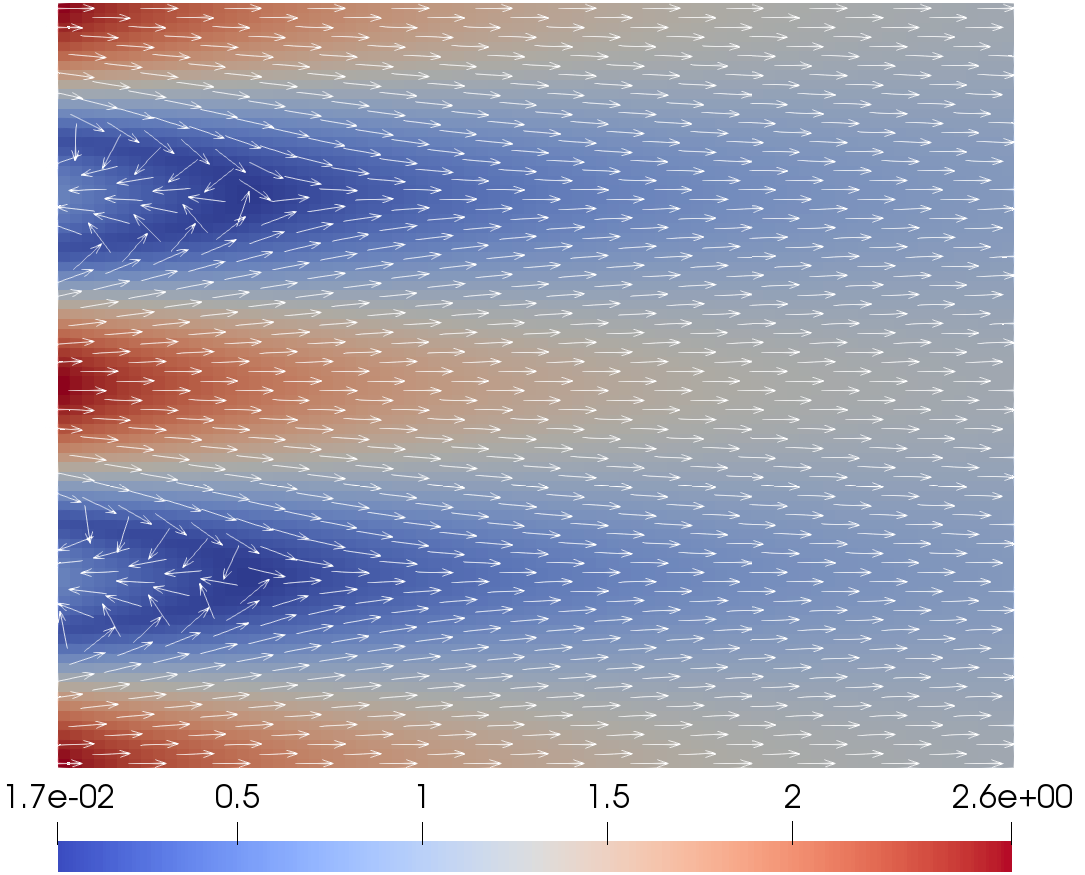
\includegraphics[width=0.5\textwidth]{kov_exact_v.png}}
	\subfloat{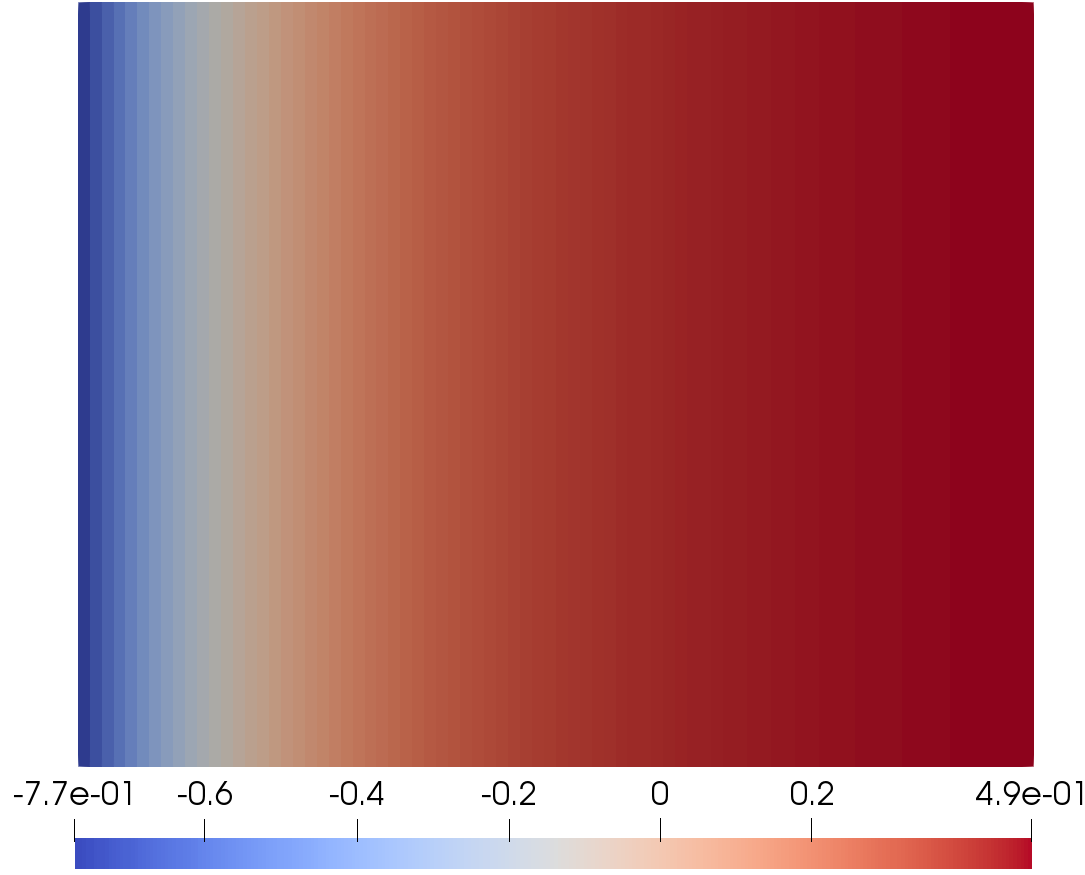
\includegraphics[width=0.5\textwidth]{kov_exact_p.png}}
	\caption[Exact solution of the Kovasznay test]{Exact solution of the 
	Kovasznay test \eqref{eq:uexkov}--\eqref{eq:pexkov}. On the left the 
	magnitude of the velocity field, on the 
	right the pressure field. The arrows are not scaled.}
	\label{fig:kovexact}
\end{figure}

The problem is solved over a sequence of seven uniform grids, starting from 
$\num{4x4}$ cells and each time halving their size. Both the cases of 
$\nu=\num{2.5e-2}$ and $\nu=\num{2.5e-4}$ are considered, that correspond respectively to 
$Re=80$ and $Re=\num{8e3}$. In Figure~\ref{fig:kov_err} the errors 
computed are reported depending on the number of cells, while in 
Table~\ref{tab:kov} we can compare directly the 
convergence orders for the different differencing schemes.
\begin{figure}
	\centering
	\subfloat[Upwind, $Re = 80$]{
		% This file was created by matlab2tikz.
%
\definecolor{mycolor1}{rgb}{0.00000,0.44700,0.74100}%
\definecolor{mycolor2}{rgb}{0.85000,0.32500,0.09800}%
\definecolor{mycolor3}{rgb}{0.92900,0.69400,0.12500}%
%
\begin{tikzpicture}

\begin{axis}[%
width=0.951\figwidth,
height=0.75\figwidth,
at={(0\figwidth,0\figwidth)},
scale only axis,
xmode=log,
xmin=4,
xmax=256,
xminorticks=true,
ymode=log,
ymin=0.000651880984,
ymax=1,
yminorticks=true,
axis background/.style={fill=white},
legend style={at={(0.03,0.03)}, anchor=south west, legend cell align=left, align=left, draw=white!15!black}
]
\addplot [color=mycolor1, mark=x, mark options={solid, mycolor1}]
  table[row sep=crcr]{%
4	0.463423878\\
8	0.143112573\\
16	0.0498339933\\
32	0.0274485113\\
64	0.0157273343\\
128	0.00905807802\\
256	0.00511952099\\
};
\addlegendentry{$p$}

\addplot [color=mycolor2, mark=x, mark options={solid, mycolor2}]
  table[row sep=crcr]{%
4	0.0365475504\\
8	0.0402359415\\
16	0.0284971904\\
32	0.016030142\\
64	0.00911637277\\
128	0.00494934791\\
256	0.00260057897\\
};
\addlegendentry{$u$}

\addplot [color=mycolor3, mark=x, mark options={solid, mycolor3}]
  table[row sep=crcr]{%
4	0.01620299\\
8	0.0203942699\\
16	0.00813891576\\
32	0.00425163801\\
64	0.00234145986\\
128	0.00125075128\\
256	0.000651880984\\
};
\addlegendentry{$v$}

\addplot [color=white!70!black, forget plot]
  table[row sep=crcr]{%
4	0.041720382976\\
256	0.000651880984\\
};
\addplot [color=white!70!black, forget plot]
  table[row sep=crcr]
	\subfloat[Upwind, $Re = \num{8e3}$]{
		% This file was created by matlab2tikz.
%
\definecolor{mycolor1}{rgb}{0.00000,0.44700,0.74100}%
\definecolor{mycolor2}{rgb}{0.85000,0.32500,0.09800}%
\definecolor{mycolor3}{rgb}{0.92900,0.69400,0.12500}%
%
\begin{tikzpicture}

\begin{axis}[%
width=0.951\figwidth,
height=0.75\figwidth,
at={(0\figwidth,0\figwidth)},
scale only axis,
xmode=log,
xmin=4,
xmax=256,
xminorticks=true,
ymode=log,
ymin=5.06127924e-05,
ymax=0.0108188379,
yminorticks=true,
axis background/.style={fill=white},
legend style={at={(0.03,0.03)}, anchor=south west, legend cell align=left, align=left, draw=white!15!black}
]
\addplot [color=mycolor1, mark=x, mark options={solid, mycolor1}]
  table[row sep=crcr]{%
4	0.0101205447\\
8	0.0108188379\\
16	0.00617459521\\
32	0.00142458715\\
64	0.00065817115\\
128	0.000326889512\\
256	0.000163405515\\
};
\addlegendentry{$p$}

\addplot [color=mycolor2, mark=x, mark options={solid, mycolor2}]
  table[row sep=crcr]{%
4	0.000827330593\\
8	0.00859442106\\
16	0.00525853983\\
32	0.00227364257\\
64	0.00103524242\\
128	0.000497944856\\
256	0.000243793246\\
};
\addlegendentry{$u$}

\addplot [color=mycolor3, mark=x, mark options={solid, mycolor3}]
  table[row sep=crcr]{%
4	0.000406472515\\
8	0.00262252421\\
16	0.00182932711\\
32	0.000454550293\\
64	0.000204199647\\
128	0.00010102046\\
256	5.06127924e-05\\
};
\addlegendentry{$v$}

\addplot [color=white!70!black, forget plot]
  table[row sep=crcr]{%
4	0.0032392187136\\
256	5.06127924e-05\\
};
\addplot [color=white!70!black, forget plot]
  table[row sep=crcr]\\
	\subfloat[Min-Mod, $Re = 80$]{
		% This file was created by matlab2tikz.
%
\definecolor{mycolor1}{rgb}{0.00000,0.44700,0.74100}%
\definecolor{mycolor2}{rgb}{0.85000,0.32500,0.09800}%
\definecolor{mycolor3}{rgb}{0.92900,0.69400,0.12500}%
%
\begin{tikzpicture}

\begin{axis}[%
width=0.951\figwidth,
height=0.75\figwidth,
at={(0\figwidth,0\figwidth)},
scale only axis,
xmode=log,
xmin=4,
xmax=256,
xminorticks=true,
ymode=log,
ymin=1e-05,
ymax=1,
yminorticks=true,
axis background/.style={fill=white},
legend style={at={(0.03,0.03)}, anchor=south west, legend cell align=left, align=left}
]
\addplot [color=mycolor1, mark=x, mark options={solid, mycolor1}]
  table[row sep=crcr]{%
4	0.465166938\\
8	0.211594301\\
16	0.136227298\\
32	0.104600388\\
64	0.0705134741\\
128	0.0412862288\\
256	0.0222713545\\
};
\addlegendentry{$p$}

\addplot [color=mycolor2, mark=x, mark options={solid, mycolor2}]
  table[row sep=crcr]{%
4	0.0370158453\\
8	0.0494417118\\
16	0.0189924822\\
32	0.0070068795\\
64	0.0018286295\\
128	0.000384013264\\
256	7.098536e-05\\
};
\addlegendentry{$u$}

\addplot [color=mycolor3, mark=x, mark options={solid, mycolor3}]
  table[row sep=crcr]{%
4	0.0169004785\\
8	0.0243528107\\
16	0.00711640549\\
32	0.00235685474\\
64	0.000570830079\\
128	0.000110084978\\
256	2.05400398e-05\\
};
\addlegendentry{$v$}

\addplot [color=white!70!black, forget plot]
  table[row sep=crcr]{%
4	0.00064\\
256	1e-05\\
};
\addplot [color=white!70!black, forget plot]
  table[row sep=crcr]
	\subfloat[Min-Mod, $Re = \num{8e3}$]{
		% This file was created by matlab2tikz.
%
\definecolor{mycolor1}{rgb}{0.00000,0.44700,0.74100}%
\definecolor{mycolor2}{rgb}{0.85000,0.32500,0.09800}%
\definecolor{mycolor3}{rgb}{0.92900,0.69400,0.12500}%
%
\begin{tikzpicture}

\begin{axis}[%
width=0.951\figwidth,
height=0.75\figwidth,
at={(0\figwidth,0\figwidth)},
scale only axis,
xmode=log,
xmin=4,
xmax=256,
xminorticks=true,
ymode=log,
ymin=1e-06,
ymax=0.010134474,
yminorticks=true,
axis background/.style={fill=white},
legend style={at={(0.03,0.03)}, anchor=south west, legend cell align=left, align=left}
]
\addplot [color=mycolor1, mark=x, mark options={solid, mycolor1}]
  table[row sep=crcr]{%
4	0.010134474\\
8	0.00824868818\\
16	0.00116892786\\
32	0.000702043982\\
64	0.000420463449\\
128	0.000239681668\\
256	0.000127809753\\
};
\addlegendentry{$p$}

\addplot [color=mycolor2, mark=x, mark options={solid, mycolor2}]
  table[row sep=crcr]{%
4	0.000766547494\\
8	0.00735792955\\
16	0.000706862636\\
32	0.00061606567\\
64	0.000254939342\\
128	9.30517021e-05\\
256	2.60788059e-05\\
};
\addlegendentry{$u$}

\addplot [color=mycolor3, mark=x, mark options={solid, mycolor3}]
  table[row sep=crcr]{%
4	0.000402295852\\
8	0.00251081251\\
16	0.000178010463\\
32	0.000121323939\\
64	4.65005959e-05\\
128	1.42957502e-05\\
256	3.67281348e-06\\
};
\addlegendentry{$v$}

\addplot [color=white!70!black, forget plot]
  table[row sep=crcr]{%
4	6.4e-05\\
256	1e-06\\
};
\addplot [color=white!70!black, forget plot]
  table[row sep=crcr]\\
	\subfloat[Van Leer, $Re = 80$]{
		% This file was created by matlab2tikz.
%
\definecolor{mycolor1}{rgb}{0.00000,0.44700,0.74100}%
\definecolor{mycolor2}{rgb}{0.85000,0.32500,0.09800}%
\definecolor{mycolor3}{rgb}{0.92900,0.69400,0.12500}%
%
\begin{tikzpicture}

\begin{axis}[%
width=0.951\figwidth,
height=0.75\figwidth,
at={(0\figwidth,0\figwidth)},
scale only axis,
xmode=log,
xmin=4,
xmax=256,
xminorticks=true,
ymode=log,
ymin=1e-05,
ymax=1,
yminorticks=true,
axis background/.style={fill=white},
legend style={at={(0.03,0.03)}, anchor=south west, legend cell align=left, align=left, draw=white!15!black}
]
\addplot [color=mycolor1, mark=x, mark options={solid, mycolor1}]
  table[row sep=crcr]{%
4	0.465362151\\
8	0.217919739\\
16	0.139676226\\
32	0.108111944\\
64	0.0720073262\\
128	0.041719522\\
256	0.0223197113\\
};
\addlegendentry{$p$}

\addplot [color=mycolor2, mark=x, mark options={solid, mycolor2}]
  table[row sep=crcr]{%
4	0.0369687113\\
8	0.0508536301\\
16	0.0240504197\\
32	0.00891876699\\
64	0.00230043057\\
128	0.000492539951\\
256	9.46578832e-05\\
};
\addlegendentry{$u$}

\addplot [color=mycolor3, mark=x, mark options={solid, mycolor3}]
  table[row sep=crcr]{%
4	0.0170184173\\
8	0.0249081905\\
16	0.00786909699\\
32	0.00254735352\\
64	0.000629680162\\
128	0.000123018505\\
256	2.07816951e-05\\
};
\addlegendentry{$v$}

\addplot [color=white!70!black, forget plot]
  table[row sep=crcr]{%
4	0.00064\\
256	1e-05\\
};
\addplot [color=white!70!black, forget plot]
  table[row sep=crcr]
	\subfloat[Van Leer, $Re = \num{8e3}$]{
		% This file was created by matlab2tikz.
%
\definecolor{mycolor1}{rgb}{0.00000,0.44700,0.74100}%
\definecolor{mycolor2}{rgb}{0.85000,0.32500,0.09800}%
\definecolor{mycolor3}{rgb}{0.92900,0.69400,0.12500}%
%
\begin{tikzpicture}

\begin{axis}[%
width=0.951\figwidth,
height=0.75\figwidth,
at={(0\figwidth,0\figwidth)},
scale only axis,
xmode=log,
xmin=4,
xmax=256,
xminorticks=true,
ymode=log,
ymin=1e-06,
ymax=0.010132924,
yminorticks=true,
axis background/.style={fill=white},
legend style={at={(0.03,0.03)}, anchor=south west, legend cell align=left, align=left}
]
\addplot [color=mycolor1, mark=x, mark options={solid, mycolor1}]
  table[row sep=crcr]{%
4	0.010132924\\
8	0.00680316149\\
16	0.000677901356\\
32	0.000521130225\\
64	0.000372827168\\
128	0.000226965042\\
256	0.000124578854\\
};
\addlegendentry{$p$}

\addplot [color=mycolor2, mark=x, mark options={solid, mycolor2}]
  table[row sep=crcr]{%
4	0.000752792347\\
8	0.00792052753\\
16	0.000772150807\\
32	0.000461995506\\
64	0.000232426927\\
128	8.93024538e-05\\
256	2.52578072e-05\\
};
\addlegendentry{$u$}

\addplot [color=mycolor3, mark=x, mark options={solid, mycolor3}]
  table[row sep=crcr]{%
4	0.00040159829\\
8	0.00256437192\\
16	0.000197529591\\
32	0.000108825618\\
64	4.65481791e-05\\
128	1.4700347e-05\\
256	3.78297463e-06\\
};
\addlegendentry{$v$}

\addplot [color=white!70!black, forget plot]
  table[row sep=crcr]{%
4	6.4e-05\\
256	1e-06\\
};
\addplot [color=white!70!black, forget plot]
  table[row sep=crcr]
	\caption[$L^2(\Omega)$ norm of the errors for the Kovasznay 
	test]{$L^2(\Omega)$ norm of the errors for the 
	Kovasznay test depending on the number of cells in the grid. The grey 
	lines are the reference lines for the first-order (lower) and second-order 
	(upper) convergence.}
	\label{fig:kov_err}
\end{figure}
\begin{table}
	\centering
	\subfloat[$Re=80$]{
	$\begin{array}{c|ccc}
	\toprule
	& \text{Upwind} & \text{Min-Mod} & \text{Van Leer} \\ 
	\midrule
	p & 0.823 & 0.890 & 0.902\\
	u & 0.928 & 2.436 & 2.379\\
	v & 0.940 & 2.422 & 2.565\\
	\bottomrule
	\end{array}
	\label{tab:kov_lre}$
	}\\
	\subfloat[$Re=\num{8e3}$]{
	$\begin{array}{c|ccc}
	\toprule
	& \text{Upwind} & \text{Min-Mod} & \text{Van Leer} \\ 
	\midrule
	p & 1.000 & 0.907 & 0.865\\
	u & 1.030 & 1.835 & 1.822\\
	v & 0.997 & 1.960 & 1.958\\
	\bottomrule
	\end{array}
	\label{tab:kov_hre}$
	}
	\caption[Convergence orders for the Kovasznay 
	test]{Convergence orders with for the Kovasznay 
	test. They are computed considering the last two refinements of the 
	grid.}
	\label{tab:kov}
\end{table}

From Table~\ref{tab:kov}, we see that in this test 
the convergence results for $Re=80$ and $Re=\num{8e3}$ are very similar. With 
the upwind method the convergence orders are always 1, while with the TVD 
methods we obtain a second order, but only for the velocity. However, observing 
Figure~\ref{fig:kov_err}, the convergence orders for the TVD methods at 
$Re=\num{8e3}$ are increasing in the last four refinements.
%
%\section{Angeli test}

\backmatter
\nocite{*}
%\printbibliography[heading=bibintoc]
\end{document}
